\documentclass{beamer}
\usepackage{tikz}
\usetheme{Madrid}
\usepackage[utf8]{inputenc}

\usepackage[T1]{fontenc} % za đ
\usepackage{gensymb}
\usepackage{amssymb}
\usepackage{amsmath}
\usepackage{graphicx}
\usepackage{subcaption}
\graphicspath{ {./images/} }
\usepackage{mathtools}
\usepackage{pgf-pie}

\usepackage{amsmath,amssymb}

\setbeamertemplate{frametitle continuation}{}
\newtheorem{primer}{Primer}[section]


%%%%%%%%%%%%%%%%%%%%%%%%%%%%%%%%%%%%%%%%%%%%%%%%%%%%%%%%%%%%%%%%%%%%%%%%%%%%%%

\DeclarePairedDelimiter\abs{\lvert}{\rvert}% za apsolutnu vrednost

%%%%%%%%%%%%%%%%%%%%%%%%%%%%%%%%%%%%%%%%%%%%%%%%%%%%%%%%%%%%%%%%%%%%%%%%%%%%%%

\renewcommand\contentsname{Content}

%%%%%%%%%%%%%%%%%%%%%%%%%%%%%%%%%%%%%%%%%%%%%%%%%%%%%%%%%%%%%%%%%%%%%%%%%%%%%%

\title{Introduction \& Test results}
\author[Milica Simić]{Milica Simić}
\centering
\date{November 2023}

\usepackage{biblatex}
%\usepackage{natbib}
%\renewcommand{\refname}{Literatura}

\addbibresource{ref.bib}
\nocite{*}
%%%%%%%%%%%%%%%%%%%%%%%%%%%%%%%%%%%%%%%%%%%%%%%%%%%%%%%%%%%%%%%%%%%%%%%%%%%%%%

\begin{document}
\maketitle

%%%%%%%%%%%%%%%%%%%%%%%%%%%%%%%%%%%%%%%%%%%%%%%%%%%%%%%%%%%%%%%%%%%%%%%%%%%%%%
%%%%%%%%%%%%%%%%%%%%%%%%%%%%%%%%%%%%%%%%%%%%%%%%%%%%%%%%%%%%%%%%%%%%%%%%%%%%%%

\begin{frame}{Content}

\tableofcontents

\end{frame}
%%%%%%%%%%%%%%%%%%%%%%%%%%%%%%%%%%%%%%%%%%%%%%%%%%%%%%%%%%%%%%%%%%%%%%%%%%%%%%
\section{Introduction}
\begin{frame}{Introduction}

\begin{itemize}
    \item<1-> Educational background: Completed a master’s degree at the University of Belgrade’s Faculty of Mathematics, specializing in mathematics and computer science
    \item<2-> Current employment: Working at Endava where our client is Adobe
    \item<3-> Career aspiration: Eager to expand knowledge in bioinformatics and actively seeking opportunities to work in a bioinformatics company
        
\end{itemize}

\end{frame}
%%%%%%%%%%%%%%%%%%%%%%%%%%%%%%%%%%%%%%%%%%%%%%%%%%%%%%%%%%%%%%%%%%%%%%%%%%%%%%
\section{Test results}
\subsection{Data}
\begin{frame}{Data}

\begin{itemize}
    \item <1->Data used in this task: Mouse embryo brain
    \item<2-> Data contains $59704$ cells and $4$ columns with values:
    \begin{itemize}
        \item<3-> cell name (\texttt{cell\_id})
        \item<4-> spatial coordinates (\texttt{x, y})
        \item<5-> cell type (\texttt{sim anno}) 
    \end{itemize}
    \item<6-> []
    \begin{columns}
        \begin{column}{0.9\textwidth} % Adjust the width as needed
          % Your image code goes here
          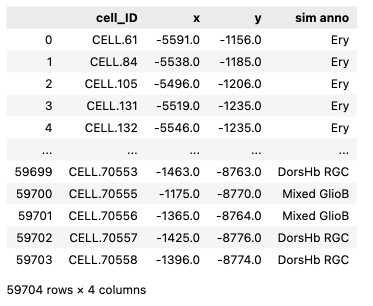
\includegraphics[width=0.5\textwidth]{dataCSV.png}
          \caption{Data in CSV format}
        \end{column}
    \end{columns}
        
\end{itemize}

\end{frame}
%%%%%%%%%%%%%%%%%%%%%%%%%%%%%%%%%%%%%%%%%%%%%%%%%%%%%%%%%%%%%%%%%%%%%%%%%%%%%%
\begin{frame}{Data}

\begin{itemize}
    \item<1-> Reduction of data was necessary due to memory and time constraints
    \item<2-> The data was filtered to remove all cells with values for x greater than $-8000$
    \item<3-> Reduced data contains $31112$ cells
    \item<4-> []
    \begin{columns}
        \begin{column}{0.9\textwidth} % Adjust the width as needed
          % Your image code goes here
          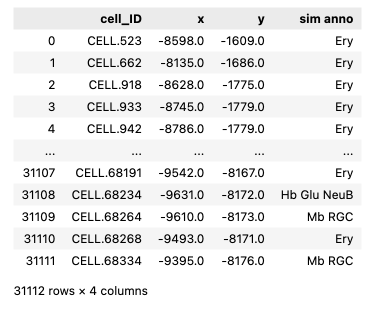
\includegraphics[width=0.55\textwidth]{reducedDataCSV.png}
          \caption{Reduced data in CSV format}
        \end{column}
    \end{columns}
        
\end{itemize}

\end{frame}
%%%%%%%%%%%%%%%%%%%%%%%%%%%%%%%%%%%%%%%%%%%%%%%%%%%%%%%%%%%%%%%%%%%%%%%%%%%%%%%
\begin{frame}{Data}

\begin{itemize}
    \item<1-> Reduced data is contained within the black rectangle
    \item<2-> []
    \begin{columns}
        \begin{column}{0.9\textwidth} % Adjust the width as needed
          % Your image code goes here
          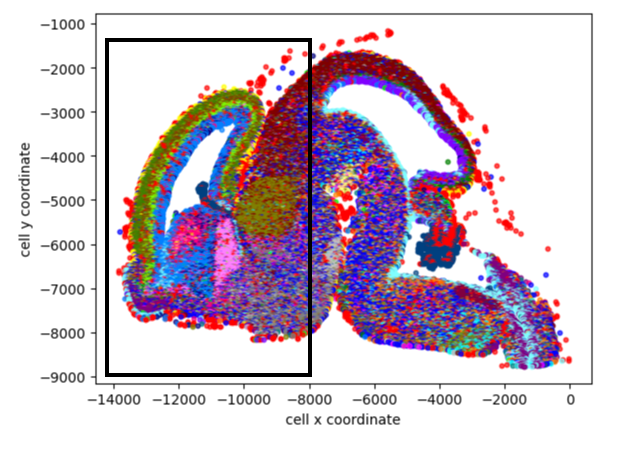
\includegraphics[width=0.7\textwidth]{reducedData.png}
          \caption{Visual representation of reduced data}
        \end{column}
    \end{columns}
        
\end{itemize}

\end{frame}
%%%%%%%%%%%%%%%%%%%%%%%%%%%%%%%%%%%%%%%%%%%%%%%%%%%%%%%%%%%%%%%%%%%%%%%%%%%%%%%
\subsection{Task}
\begin{frame}{Task}

\begin{itemize}
    \item<1-> In the context of tissue analysis, it is important to recognize that every cell within a tissue interacts with its neighboring cells, typically performing specific functions. 
    \item<2->Consequently, cells sharing similar percentage of cell types in their surroundings can be identified as spatial community
    \item<3-> The task:
    \begin{itemize}
        \item<4->  Categorize cells into spatial communities by evaluating the percentage of cell types found in their immediate surroundings
        \item<5->  Calculate the homogeneity score for each community and decide whether the community is homogeneous (community with very similar percentages of cell types in all of its parts) or heterogeneous (community in which percentages of cell types vary significantly across different parts of it)
        \item<6-> Calculate for each community the mixture (count and percentage) of cell types that are present in it
    \end{enumerate} 
\end{itemize}

\end{frame}
%%%%%%%%%%%%%%%%%%%%%%%%%%%%%%%%%%%%%%%%%%%%%%%%%%%%%%%%%%%%%%%%%%%%%%%%%%%%%%
\subsection{Adjustable parameters}
\begin{frame}{Calculation of the percentage of cell types in cell's neighborhood}

\begin{itemize}
    \item <1->Input: \texttt{Cell cell} (red dot on the image below) and \texttt{integer neighborhood\_radius} (radius of black circle on the image below)
    \item<2-> Output: \texttt{list types\_percentage}, where \texttt{types\_percentage[k]} represents the percentage of cells in the neighborhood of the cell (indicated by the black circle in the image below) that belong to the cell type with number \texttt{k}. All cell types in the tissue are mapped to integers from $0$ to \texttt{num\_of\_types - 1}
    \item<3-> []
    \begin{columns}
        \begin{column}{0.9\textwidth} % Adjust the width as needed
          % Your image code goes here
          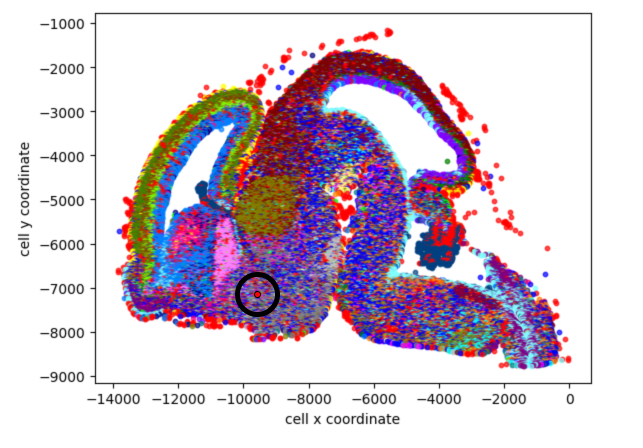
\includegraphics[width=0.35\textwidth]{radius.png}
          \caption{Neighborhood of cell}
        \end{column}
    \end{columns}
    \item<4-> After this step, we have a list of the percentage of cell types in each cell's neighborhood, allowing us to compare them based on this information
\end{itemize}

\end{frame}
%%%%%%%%%%%%%%%%%%%%%%%%%%%%%%%%%%%%%%%%%%%%%%%%%%%%%%%%%%%%%%%%%%%%%%%%%%%%%%
\begin{frame}{Comparing cells based on the percentage of cell types in their neighborhood}

\begin{itemize}
    \item<1-> Distance functions used: Manhattan, Euclidean and Hamming
    \item<2-> For the Hamming distance, there is a parameter called \texttt{hamming\_param}. For example, if \texttt{types\_percentage = [0.1, 0.5, 0.4]} and \texttt{hamming\_param = 0.3}, then the modified percentages will be \texttt{[0, 1, 1]}. In this case, only the first element ($0.1$) is less than $0.3$, so it will be set to $0$, and the rest will be set to $1$. And these modified percentages of cells will be compared when comparing two cells using the Hamming distance.
\end{itemize}

\end{frame}
%%%%%%%%%%%%%%%%%%%%%%%%%%%%%%%%%%%%%%%%%%%%%%%%%%%%%%%%%%%%%%%%%%%%%%%%%%%%%%
\begin{frame}{Clustering cells based on the similarity of cell types present in their neighborhood.}

\begin{itemize}
    \item<1-> Clustering algorithm:  Hierarchical clustering (Agglomerative) and Leiden clustering
    \item<2-> Only the results for the Agglomerative clustering will be presented, as it is better suited for the current problem
    \item<3-> For Agglomerative clustering there are two optional parameters:
    \begin{itemize}
        \item<4-> \texttt{linkage\_method} (single, average, ward, centroid) where default value is single
        \item<5-> \texttt{threshold} where default value is None, and in such cases, the optimal threshold will be calculated using the Silhouette method
    \end{itemize}
    \item<6-> Agglomerative clustering will be performed on the distance matrix \texttt{percentage\_distance\_matrix}, where \texttt{percentage\_distance\_matrix[cell\_i.id\_num][cell\_j.id\_num] = dist(cell\_i.types\_percentage, cell\_i.types\_percentage)}, and the distance function \texttt{dist} can be one of Manhattan, Euclidean, or Hamming distances
\end{itemize}

\end{frame}
%%%%%%%%%%%%%%%%%%%%%%%%%%%%%%%%%%%%%%%%%%%%%%%%%%%%%%%%%%%%%%%%%%%%%%%%%%%%%%
%%%%%%%%%%%%%%%%%%%%%%%%%%%%%%%%%%%%%%%%%%%%%%%%%%%%%%%%%%%%%%%%%%%%%%%%%%%%%%
\begin{frame}{Adjustable parameters}

\begin{itemize}
    \item<1-> In summary, the adjustable parameters are:
    \begin{itemize}
        \item<2-> \texttt{neighborhood\_radius} (mandatory parameter)
        \item<3-> \texttt{distance\_function} (Manhattan which is default, Euclidean and Hamming with parameter)
        \item<4-> \texttt{linkage\_method} (single which is default, average, ward and centroid) and \texttt{threshold} (default is None) for Agglomerative clustering
    \end{itemize}
\end{itemize}

\end{frame}
%%%%%%%%%%%%%%%%%%%%%%%%%%%%%%%%%%%%%%%%%%%%%%%%%%%%%%%%%%%%%%%%%%%%%%%%%%%%%%%
%%%%%%%%%%%%%%%%%%%%%%%%%%%%%%%%%%%%%%%%%%%%%%%%%%%%%%%%%%%%%%%%%%%%%%%%%%%%%%
\subsection{Results}
\begin{frame}{Result 1}

\begin{itemize}
    \item<1-> Results where:
    \begin{itemize}
        \item<2-> \texttt{neighborhood\_radius = 200} (the radius that corresponds to the red circle in the image below)
        \item<3-> \texttt{distance\_function = Manhattan}
        \item<4-> \texttt{linkage\_method = average}
    \end{itemize}
    \item<5-> []
    	\begin{figure}
    		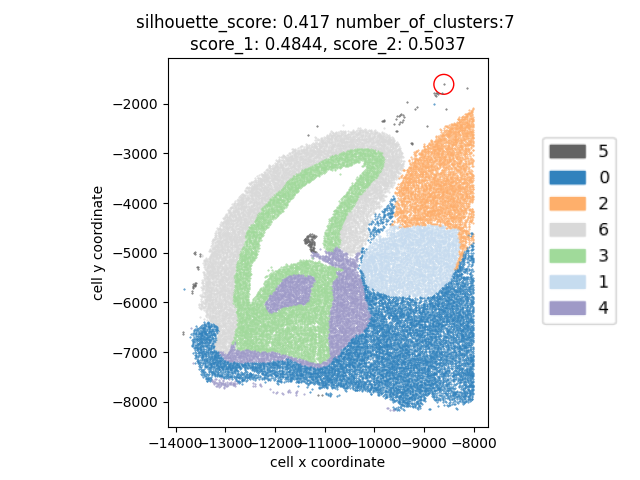
\includegraphics[width=0.55\textwidth]{clusters_2.png}
    		\caption{Clusters}
	\end{figure} 
\end{itemize}

\end{frame}
%%%%%%%%%%%%%%%%%%%%%%%%%%%%%%%%%%%%%%%%%%%%%%%%%%%%%%%%%%%%%%%%%%%%%%%%%%%%%%
\begin{frame}{Result 1 - Clusters statistics}

\begin{itemize}
    \item<1-> The mean of distribution of percentage distances between all cells is $1.48$, as shown in the image below
    \begin{figure}
    \centering
    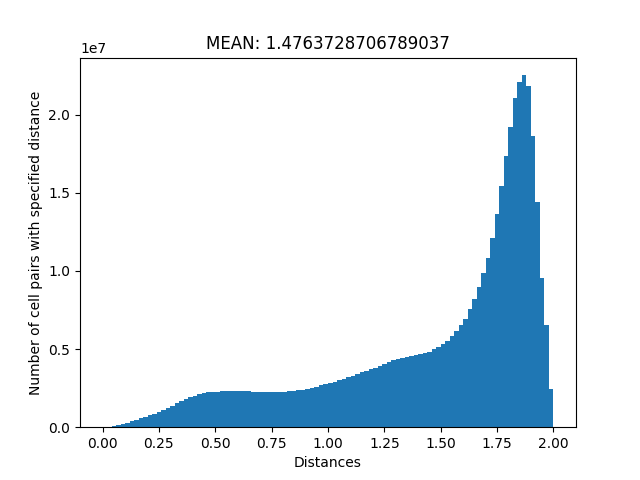
\includegraphics[width=0.7\textwidth]{all_distances2.png}
    \caption{Distribution of percentage distances between all cells}
\end{figure} 
   
\end{itemize}
\end{frame}
%%%%%%%%%%%%%%%%%%%%%%%%%%%%%%%%%%%%%%%%%%%%%%%%%%%%%%%%%%%%%%%%%%%%%%%%%%%%%%
\begin{frame}{Result 1 - Homogeneous or Heterogeneous clusters}

\begin{figure}
    \centering
    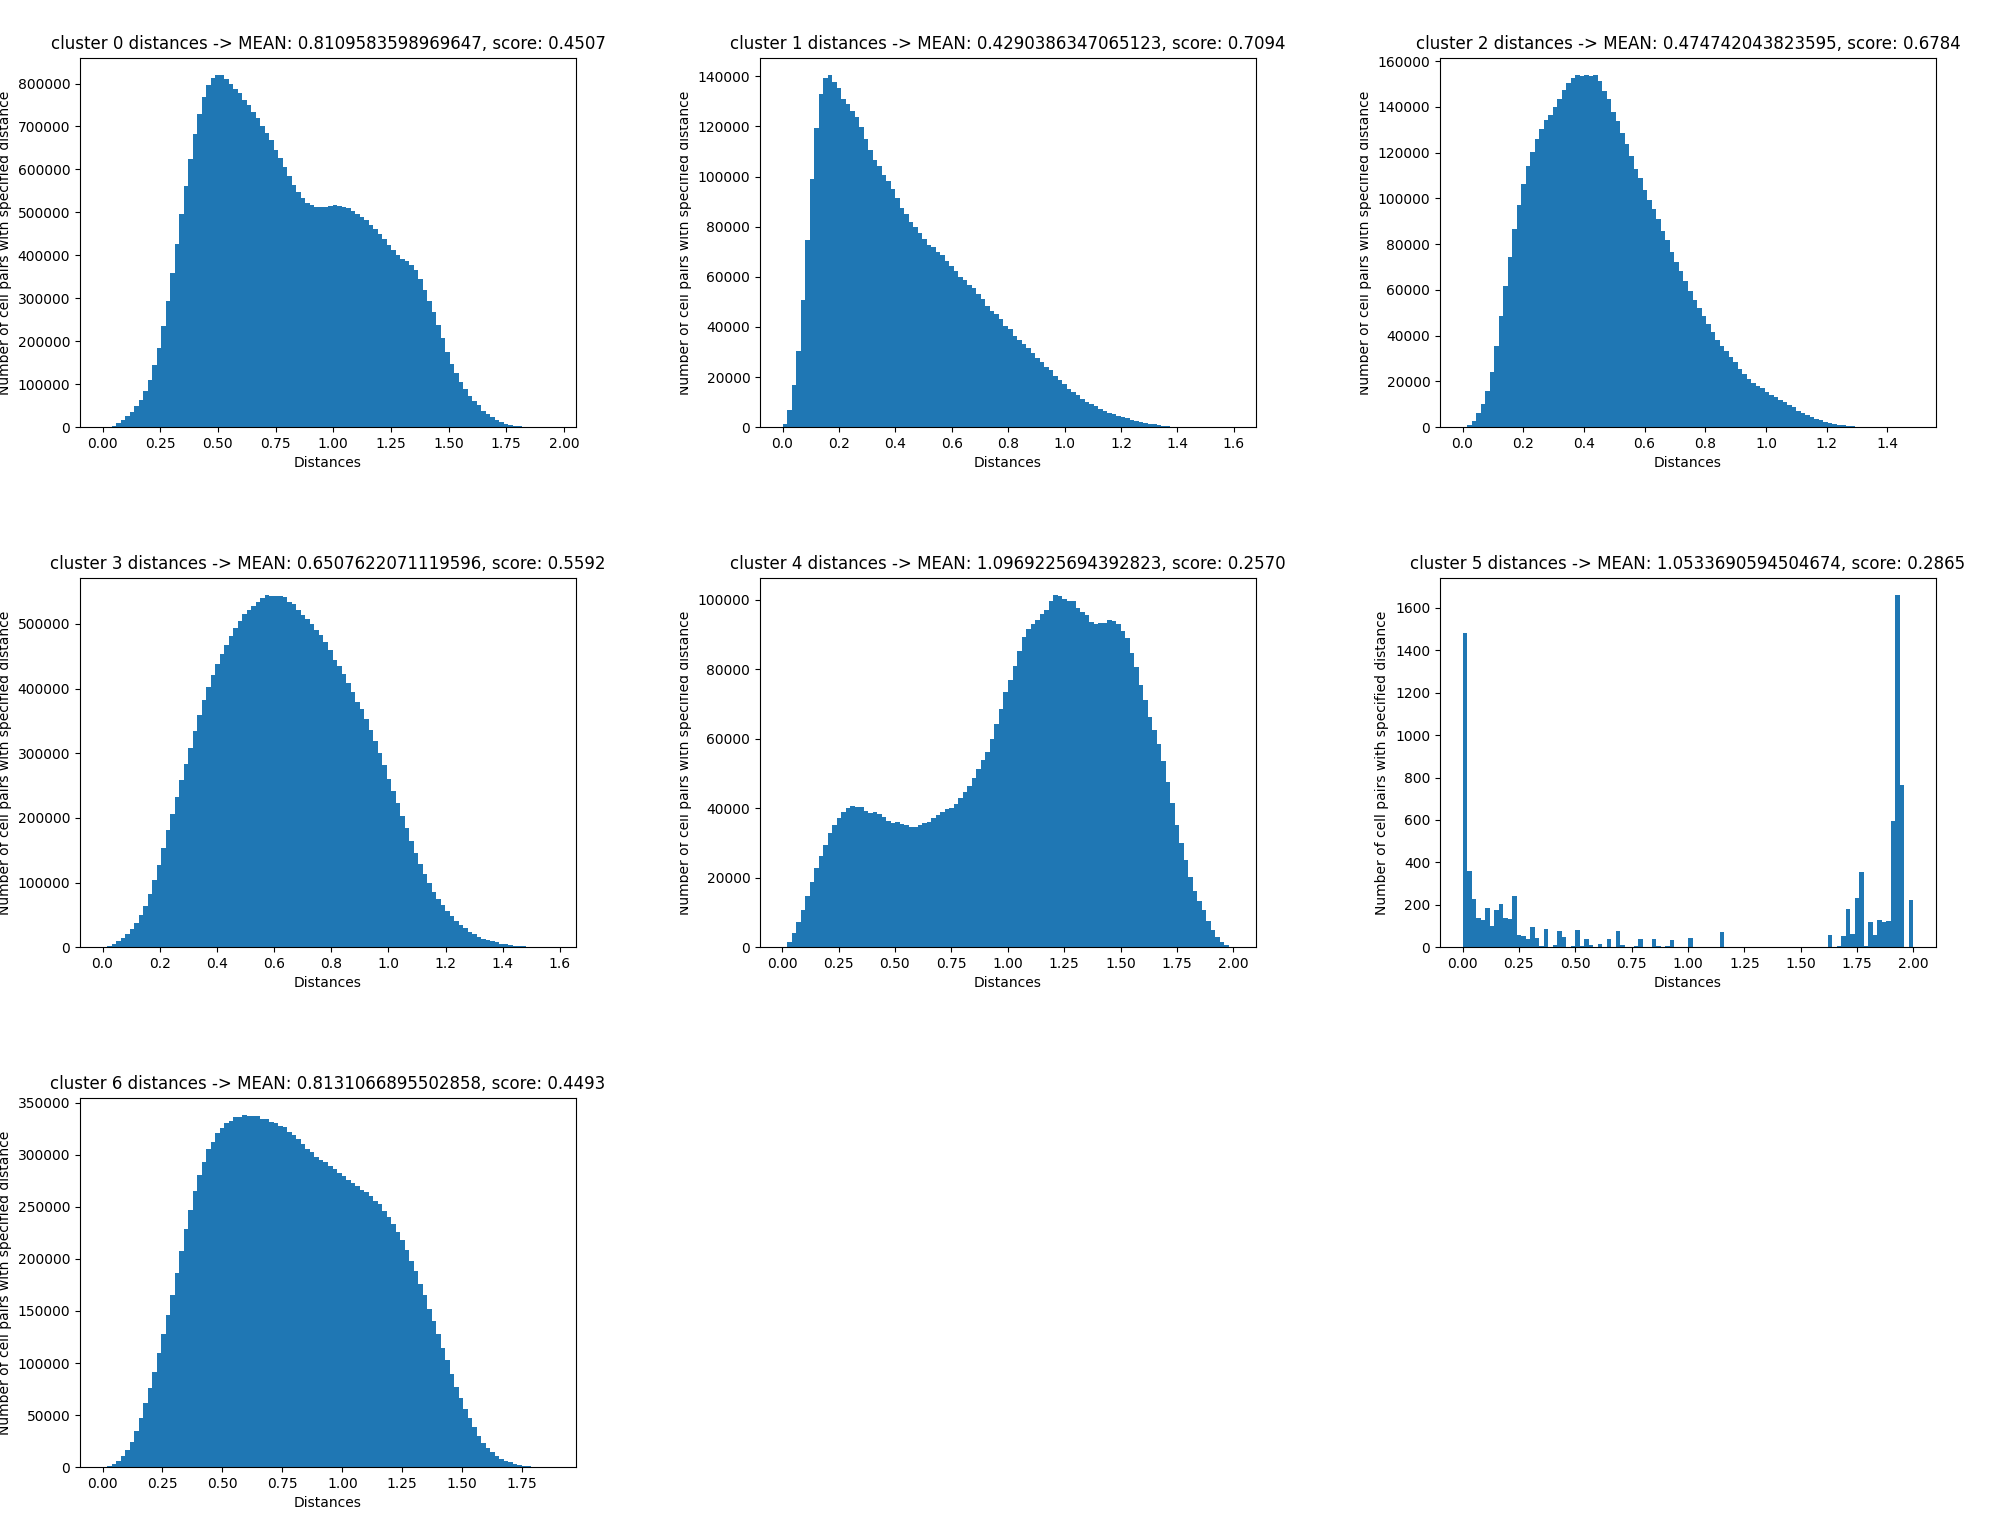
\includegraphics[width=0.7\textwidth]{stats_clusters2.png}
    \caption{Distribution of percentage distances between cells for each cluster}
\end{figure} 

\end{frame}
%%%%%%%%%%%%%%%%%%%%%%%%%%%%%%%%%%%%%%%%%%%%%%%%%%%%%%%%%%%%%%%%%%%%%%%%%%%%%%
\begin{frame}{Result 1 - Homogeneous or Heterogeneous clusters}

\begin{itemize}
    \item<1-> In the image above, distributions of percentage distances between cells for each cluster are displayed
    \item<2-> This was done to determine whether a cluster is homogeneous or heterogeneous. If a cluster is homogeneous, there should be a significant number of percentage distances between cells that are close to zero as this indicates that neighborhood of those cells are similar
    \item<3-> If there is a significant number of homogeneous clusters, it indicates the effectiveness of the clustering, as our goal is to group cells with very similar surroundings. 
    %However, this metric approach has not been fully utilized because I have not precisely defined what 'close to zero' exactly means (the value from which a certain percentage of distances within a cluster should be smaller in order for it to be considered homogeneous)
\end{itemize}
\end{frame}
%%%%%%%%%%%%%%%%%%%%%%%%%%%%%%%%%%%%%%%%%%%%%%%%%%%%%%%%%%%%%%%%%%%%%%%%%%%%%%%%%%%%%%%%%%%%%%%%%%%%%%%%%
\begin{frame}{Cluster homogeneity score}

\begin{itemize}
    \item<1-> Cluster \textit{c} homogeneity score
        \begin{equation*}
        HS(c)=
            \begin{cases}
                1 - m(c)/M &, \text{ if m(c) < M}\\
                0 &, \text{ otherwise}
            \end{cases}
        \end{equation*}
    %\[ HS(c) = 1 - m(c)/M \]
    \begin{itemize}
        \item<2-> [] \textit{m(c)} - mean of distribution of percentage distances between cells in the cluster \textit{c} 
        \item<3-> [] \textit{M} - mean of distribution of percentage distances between all cells in the tissue
    \end{itemize}
    \item<4-> Cluster homogeneity score takes values from 0 to 1 meaning:
    \begin{itemize}
        \item<5-> if \(HS(c) > 0.5\), then cluster \textit{c} is homogeneous
        \item<6-> otherwise, cluster \textit{c} is heterogeneous
    \end{itemize}
\end{itemize}
\end{frame}
%%%%%%%%%%%%%%%%%%%%%%%%%%%%%%%%%%%%%%%%%%%%%%%%%%%%%%%%%%%%%%%%%%%%%%%%%%%%%%%%%%%%%%%%%%%%%%%%%%%%%%%%%
\begin{frame}{Total homogeneity score}

\begin{itemize}
    \item<1-> Total homogeneity score of clustering C
        \[ THS(C) = \frac{\sum_{c \in C} HS(c) \cdot n(c)}{N} \]
    \begin{itemize}
        \item<2-> [] \textit{n(c)} - number of cells in the cluster \textit{c} 
        \item<3-> [] \textit{N} - number of cells in the tissue
    \end{itemize}
    \item <4-> Total homogeneity score takes values from 0 to 1 meaning: value close to 1 indicates that the clustering is of high quality, while a value close to 0 suggests that the clustering is of poor quality.
\end{itemize}
\end{frame}
%%%%%%%%%%%%%%%%%%%%%%%%%%%%%%%%%%%%%%%%%%%%%%%%%%%%%%%%%%%%%%%%%%%%%%%%%%%%%%%%%%%%%%%%%%%%%%%%%%%%%%%%%
\begin{frame}{Result 1  - Homogeneous or Heterogeneous clusters}

\begin{itemize}
    \item<1-> From the image above, we can observe that we have $7$ clusters from which $1$, $2$, and $3$ are homogeneous, and cluster $0$ and $6$ are close to homogeneous
    \item<2-> Furthermore, clusters $4$ and $5$ have the lowest homogeneity score and are heterogeneous clusters
    \item<3-> Total homogeneity score of this clustering is $0.5$ and silhouette score is $0.42$
\end{itemize}

\end{frame}
%%%%%%%%%%%%%%%%%%%%%%%%%%%%%%%%%%%%%%%%%%%%%%%%%%%%%%%%%%%%%%%%%%%%%%%%%%%%%%
\begin{frame}{Result 1 (statistics) - Number of different cell types in each cluster}

\begin{figure}
    \centering
    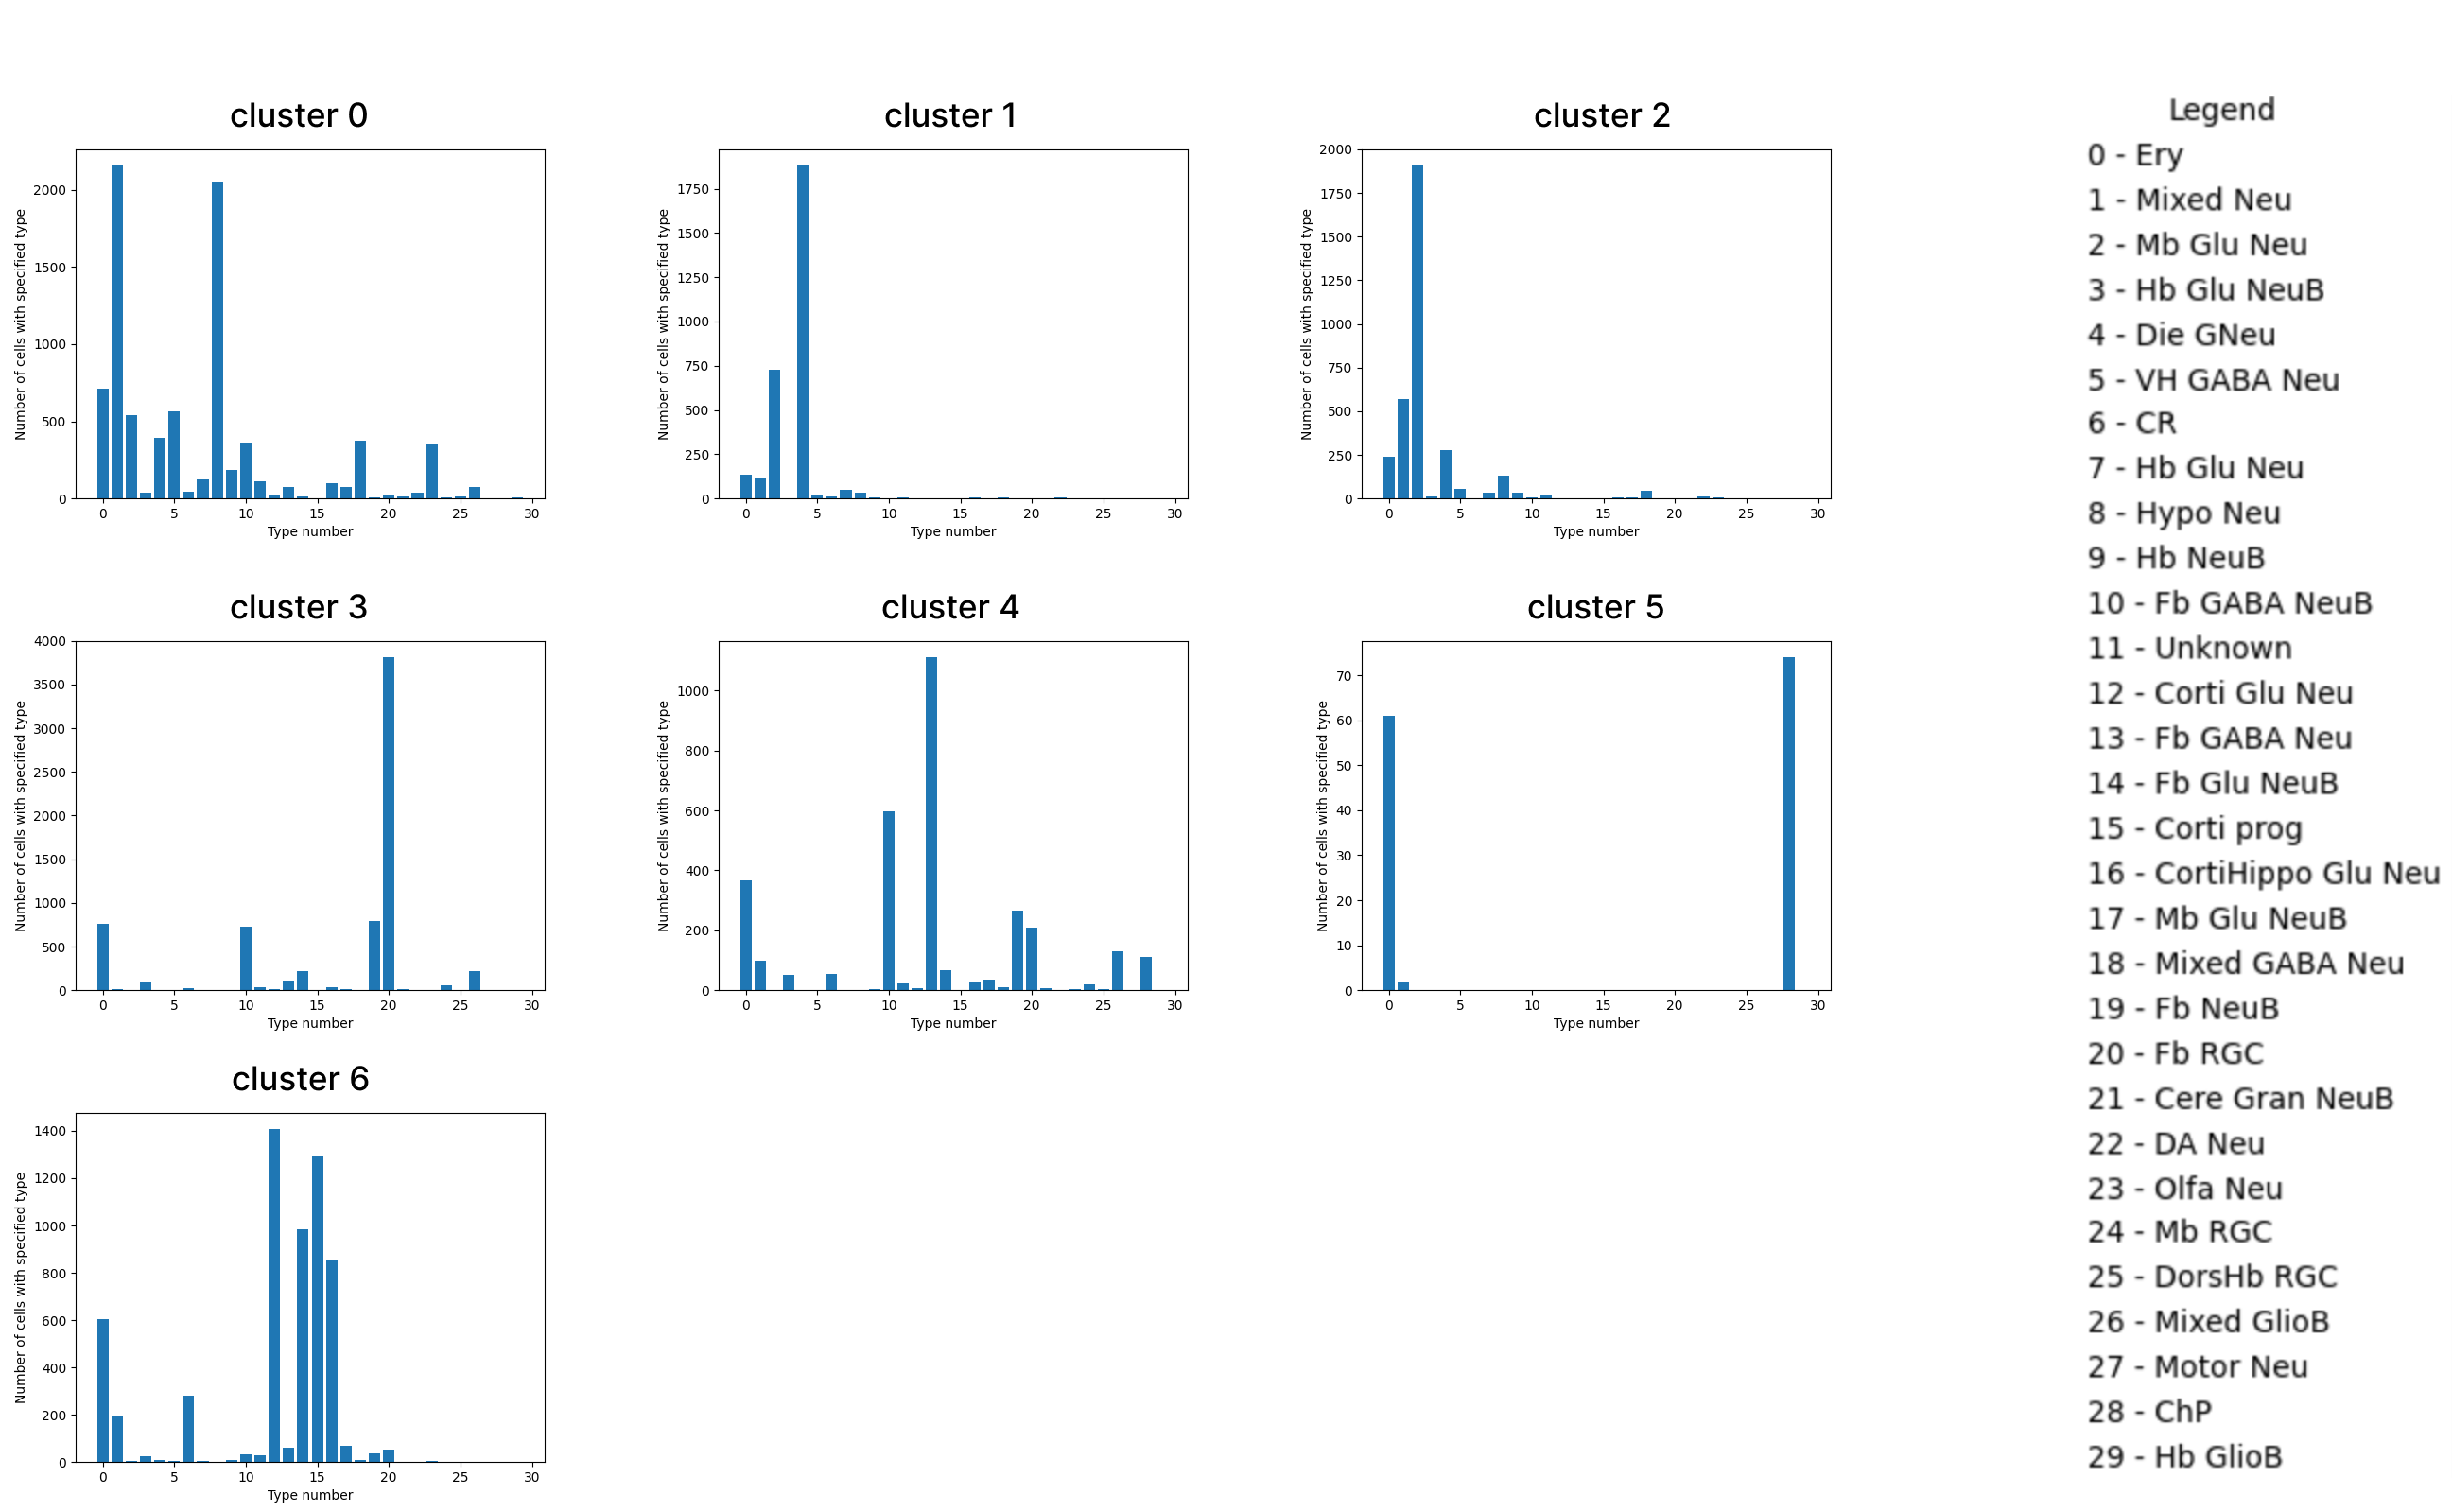
\includegraphics[width=0.8\textwidth]{type_num_clusters2.png}
    \caption{Number of different cell types in each cluster}
\end{figure} 

\end{frame}
%%%%%%%%%%%%%%%%%%%%%%%%%%%%%%%%%%%%%%%%%%%%%%%%%%%%%%%%%%%%%%%%%%%%%%%%%%%%%%
\begin{frame}{Result 1 (statistics) - Percentage of different cell types in each cluster}

\begin{figure}
    \centering
    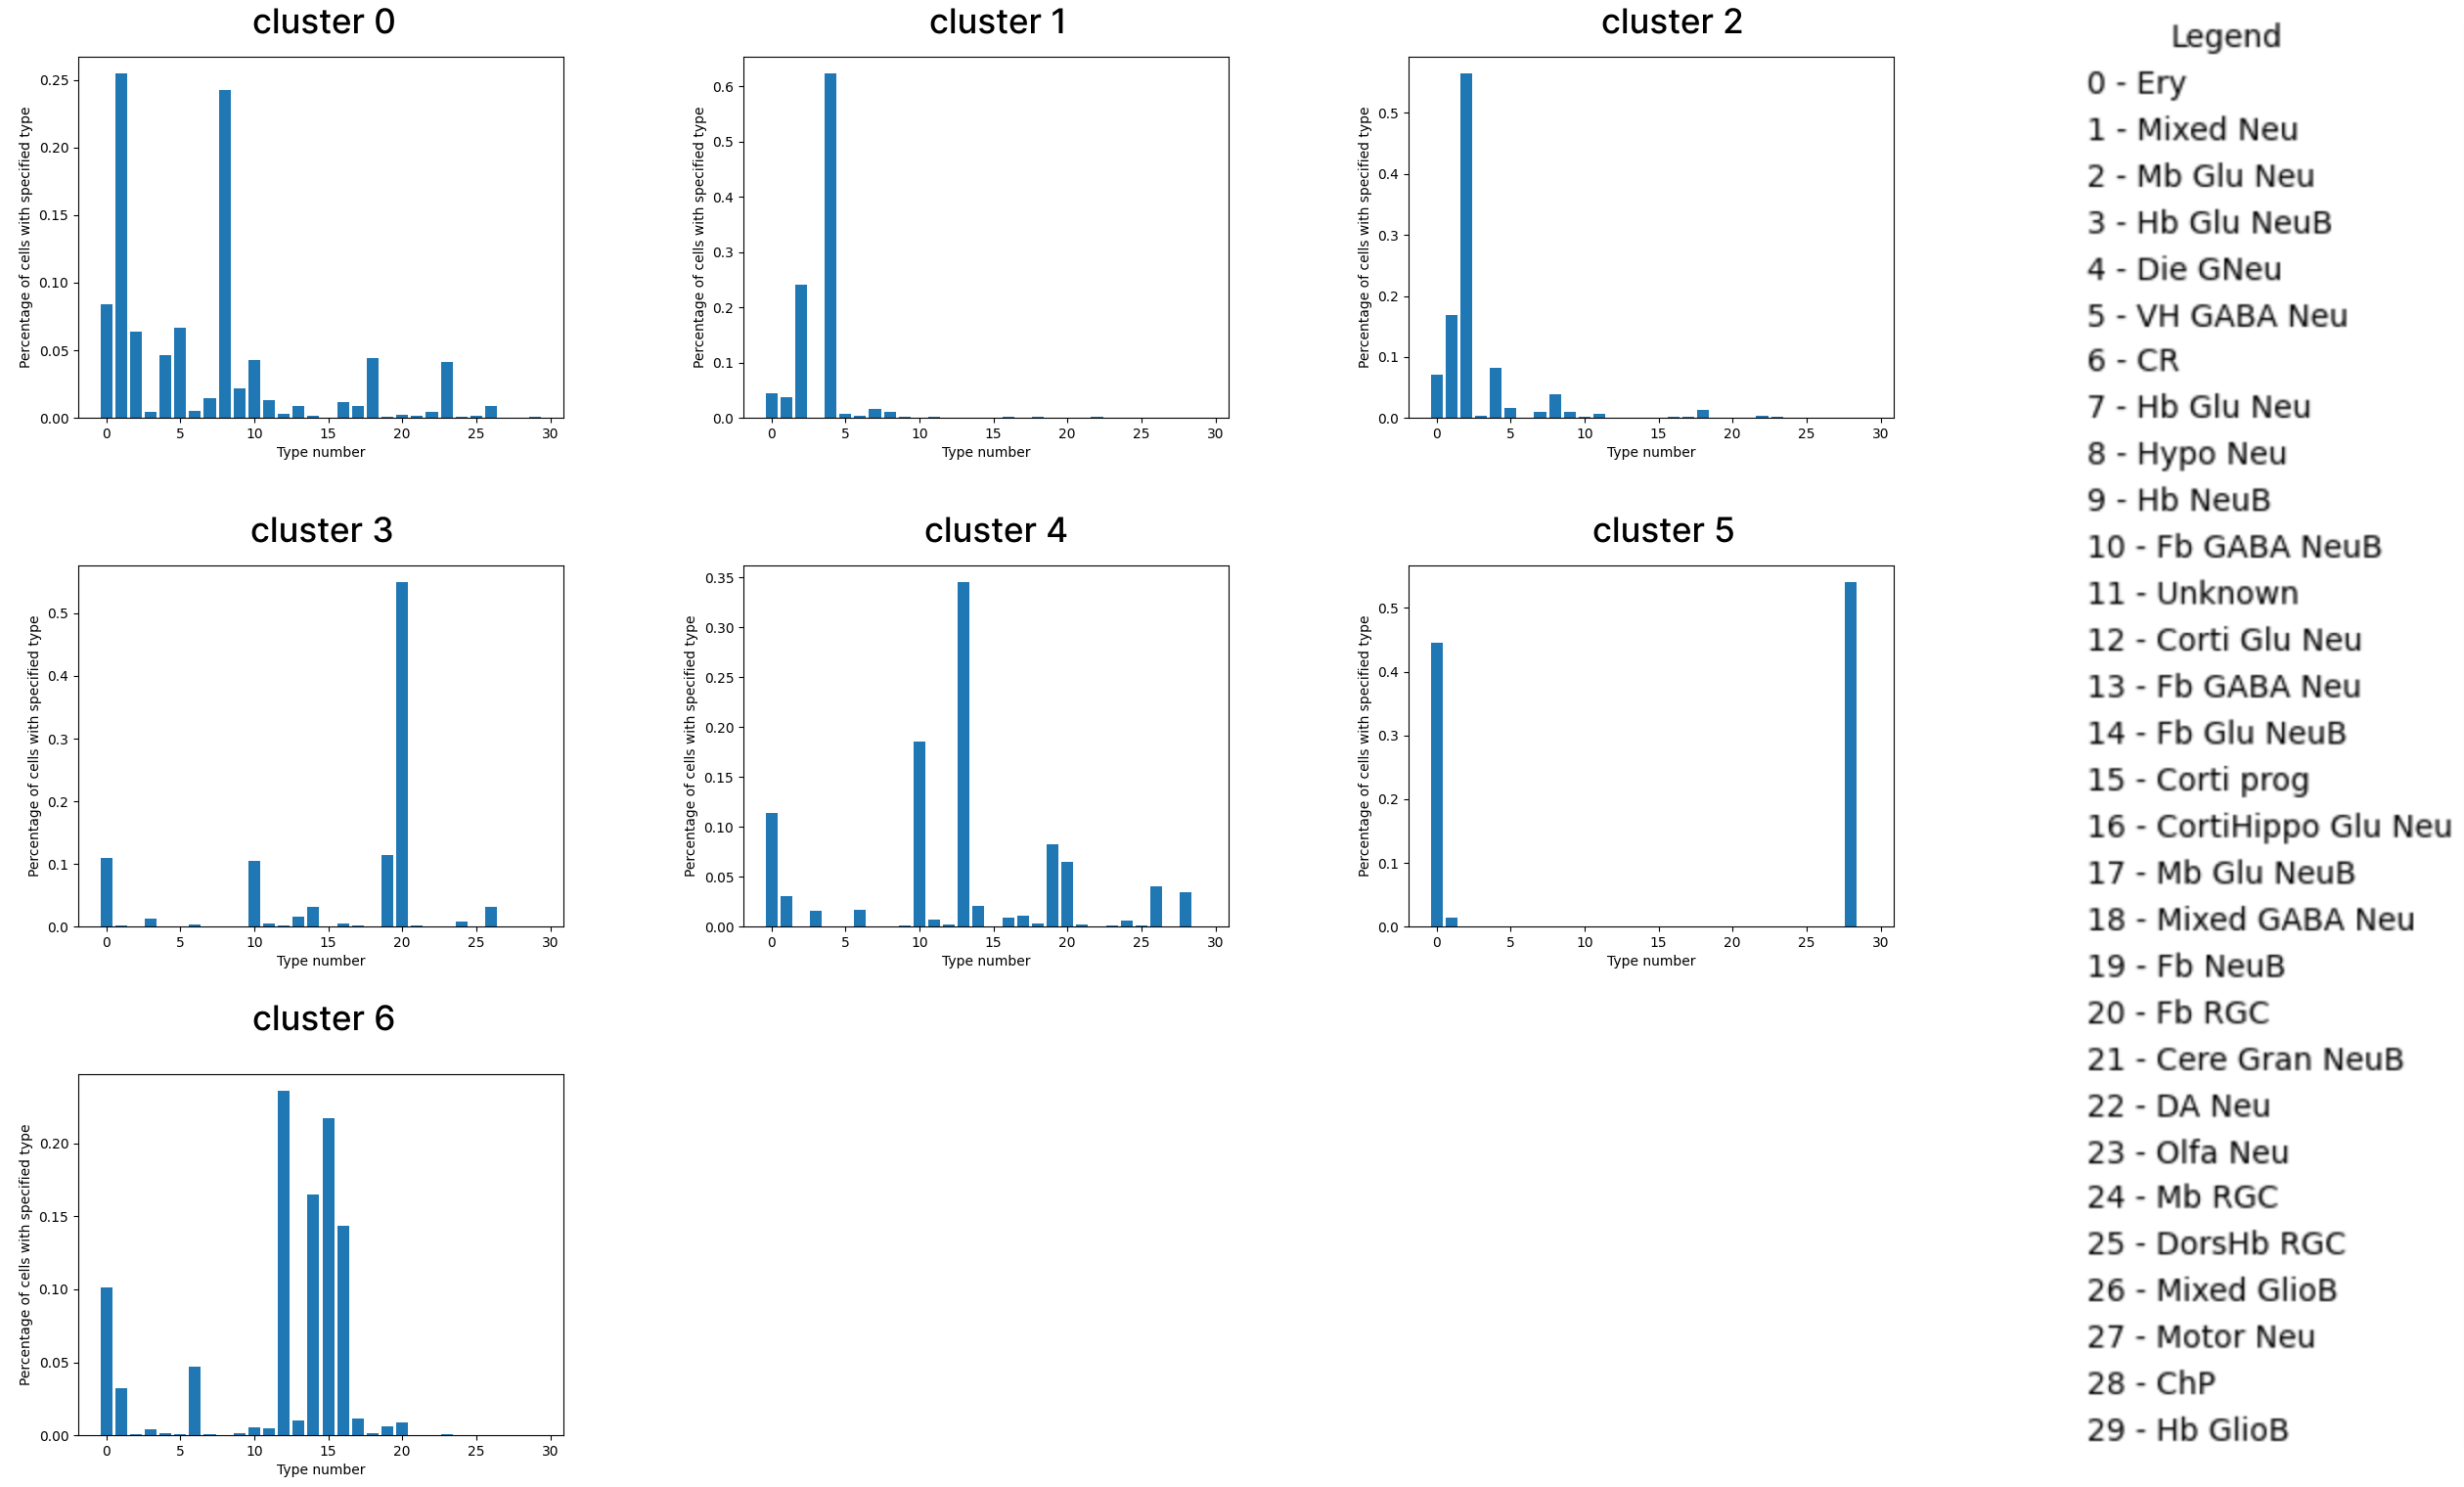
\includegraphics[width=0.8\textwidth]{type_p_clusters2.png}
    \caption{Percentage of different cell types in each cluster}
\end{figure} 

\end{frame}
%%%%%%%%%%%%%%%%%%%%%%%%%%%%%%%%%%%%%%%%%%%%%%%%%%%%%%%%%%%%%%%%%%%%%%%%%%%%%%

\begin{frame}{Result 1 - Decreasing the threshold}
\begin{itemize}
    \item<1-> []
   	 \begin{figure}
    		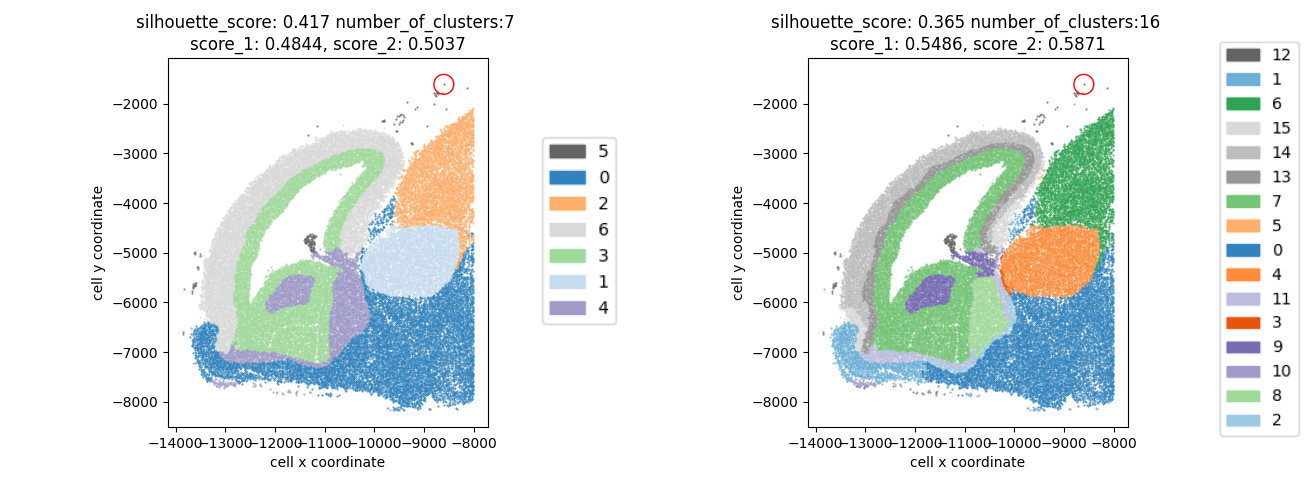
\includegraphics[width=0.6\textwidth]{clusters_1_2.png}
    		\caption{Clusters with \texttt{threshold} $64$ and $55$, respectively}
	\end{figure} 
    \item<2-> Decreasing the threshold (from $68$ to $55$) did result in a higher number of clusters with slight improvement in homogeneity score
    \item<3-> The gray cluster (cluster $6$) from the previous clustering has now been divided into clusters $13$ and $14$. This division has resulted in higher homogeneity scores for clusters $13$ ($0.62$) and $14$ ($0.6$) than what was observed for the single cluster $6$ ($0.45$) in the previous clustering. 
\end{itemize}

\end{frame}
%%%%%%%%%%%%%%%%%%%%%%%%%%%%%%%%%%%%%%%%%%%%%%%%%%%%%%%%%%%%%%%%%%%%%%%%%%%%%%
\begin{frame}{Result 1 - Decreasing the threshold}
\begin{itemize}
      \item<1-> []
     	 \begin{figure}
    		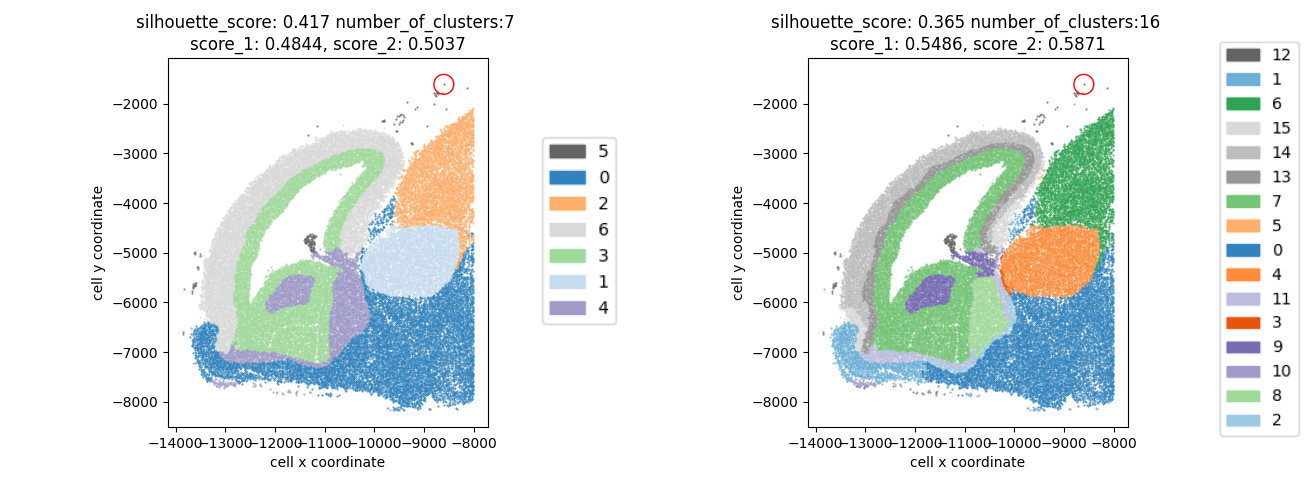
\includegraphics[width=0.45\textwidth]{clusters_1_2.png}
   		 \caption{Clusters with \texttt{threshold} $68$ and $55$, respectively}
	\end{figure} 
     \item<2-> The purple cluster (cluster $4$) from the previous clustering has now been divided into clusters $8$ , $9$ and $11$ .This division has resulted in higher homogeneity scores for clusters $8$ ($0.64$), $9$ ($0.45$) and $11$ ($0.46$) than what was observed for the single cluster $4$ ($0.26$) in the previous clustering. 
    \item<3-> The blue cluster (cluster $0$) from the previous clustering has now been divided into clusters $0$, $1$  and $2$.This division has resulted in higher homogeneity scores for clusters $0$ ($0.56$), and $2$ ($0.54$) and lower for cluster $1$ ($0.39$) than what was observed for the single cluster $0$ ($0.45$) in the previous clustering. 
\end{itemize}

\end{frame}
%%%%%%%%%%%%%%%%%%%%%%%%%%%%%%%%%%%%%%%%%%%%%%%%%%%%%%%%%%%%%%%%%%%%%%%%%%%%%%
\begin{frame}{Result 1 - Decreasing the threshold}

\begin{figure}
    \centering
    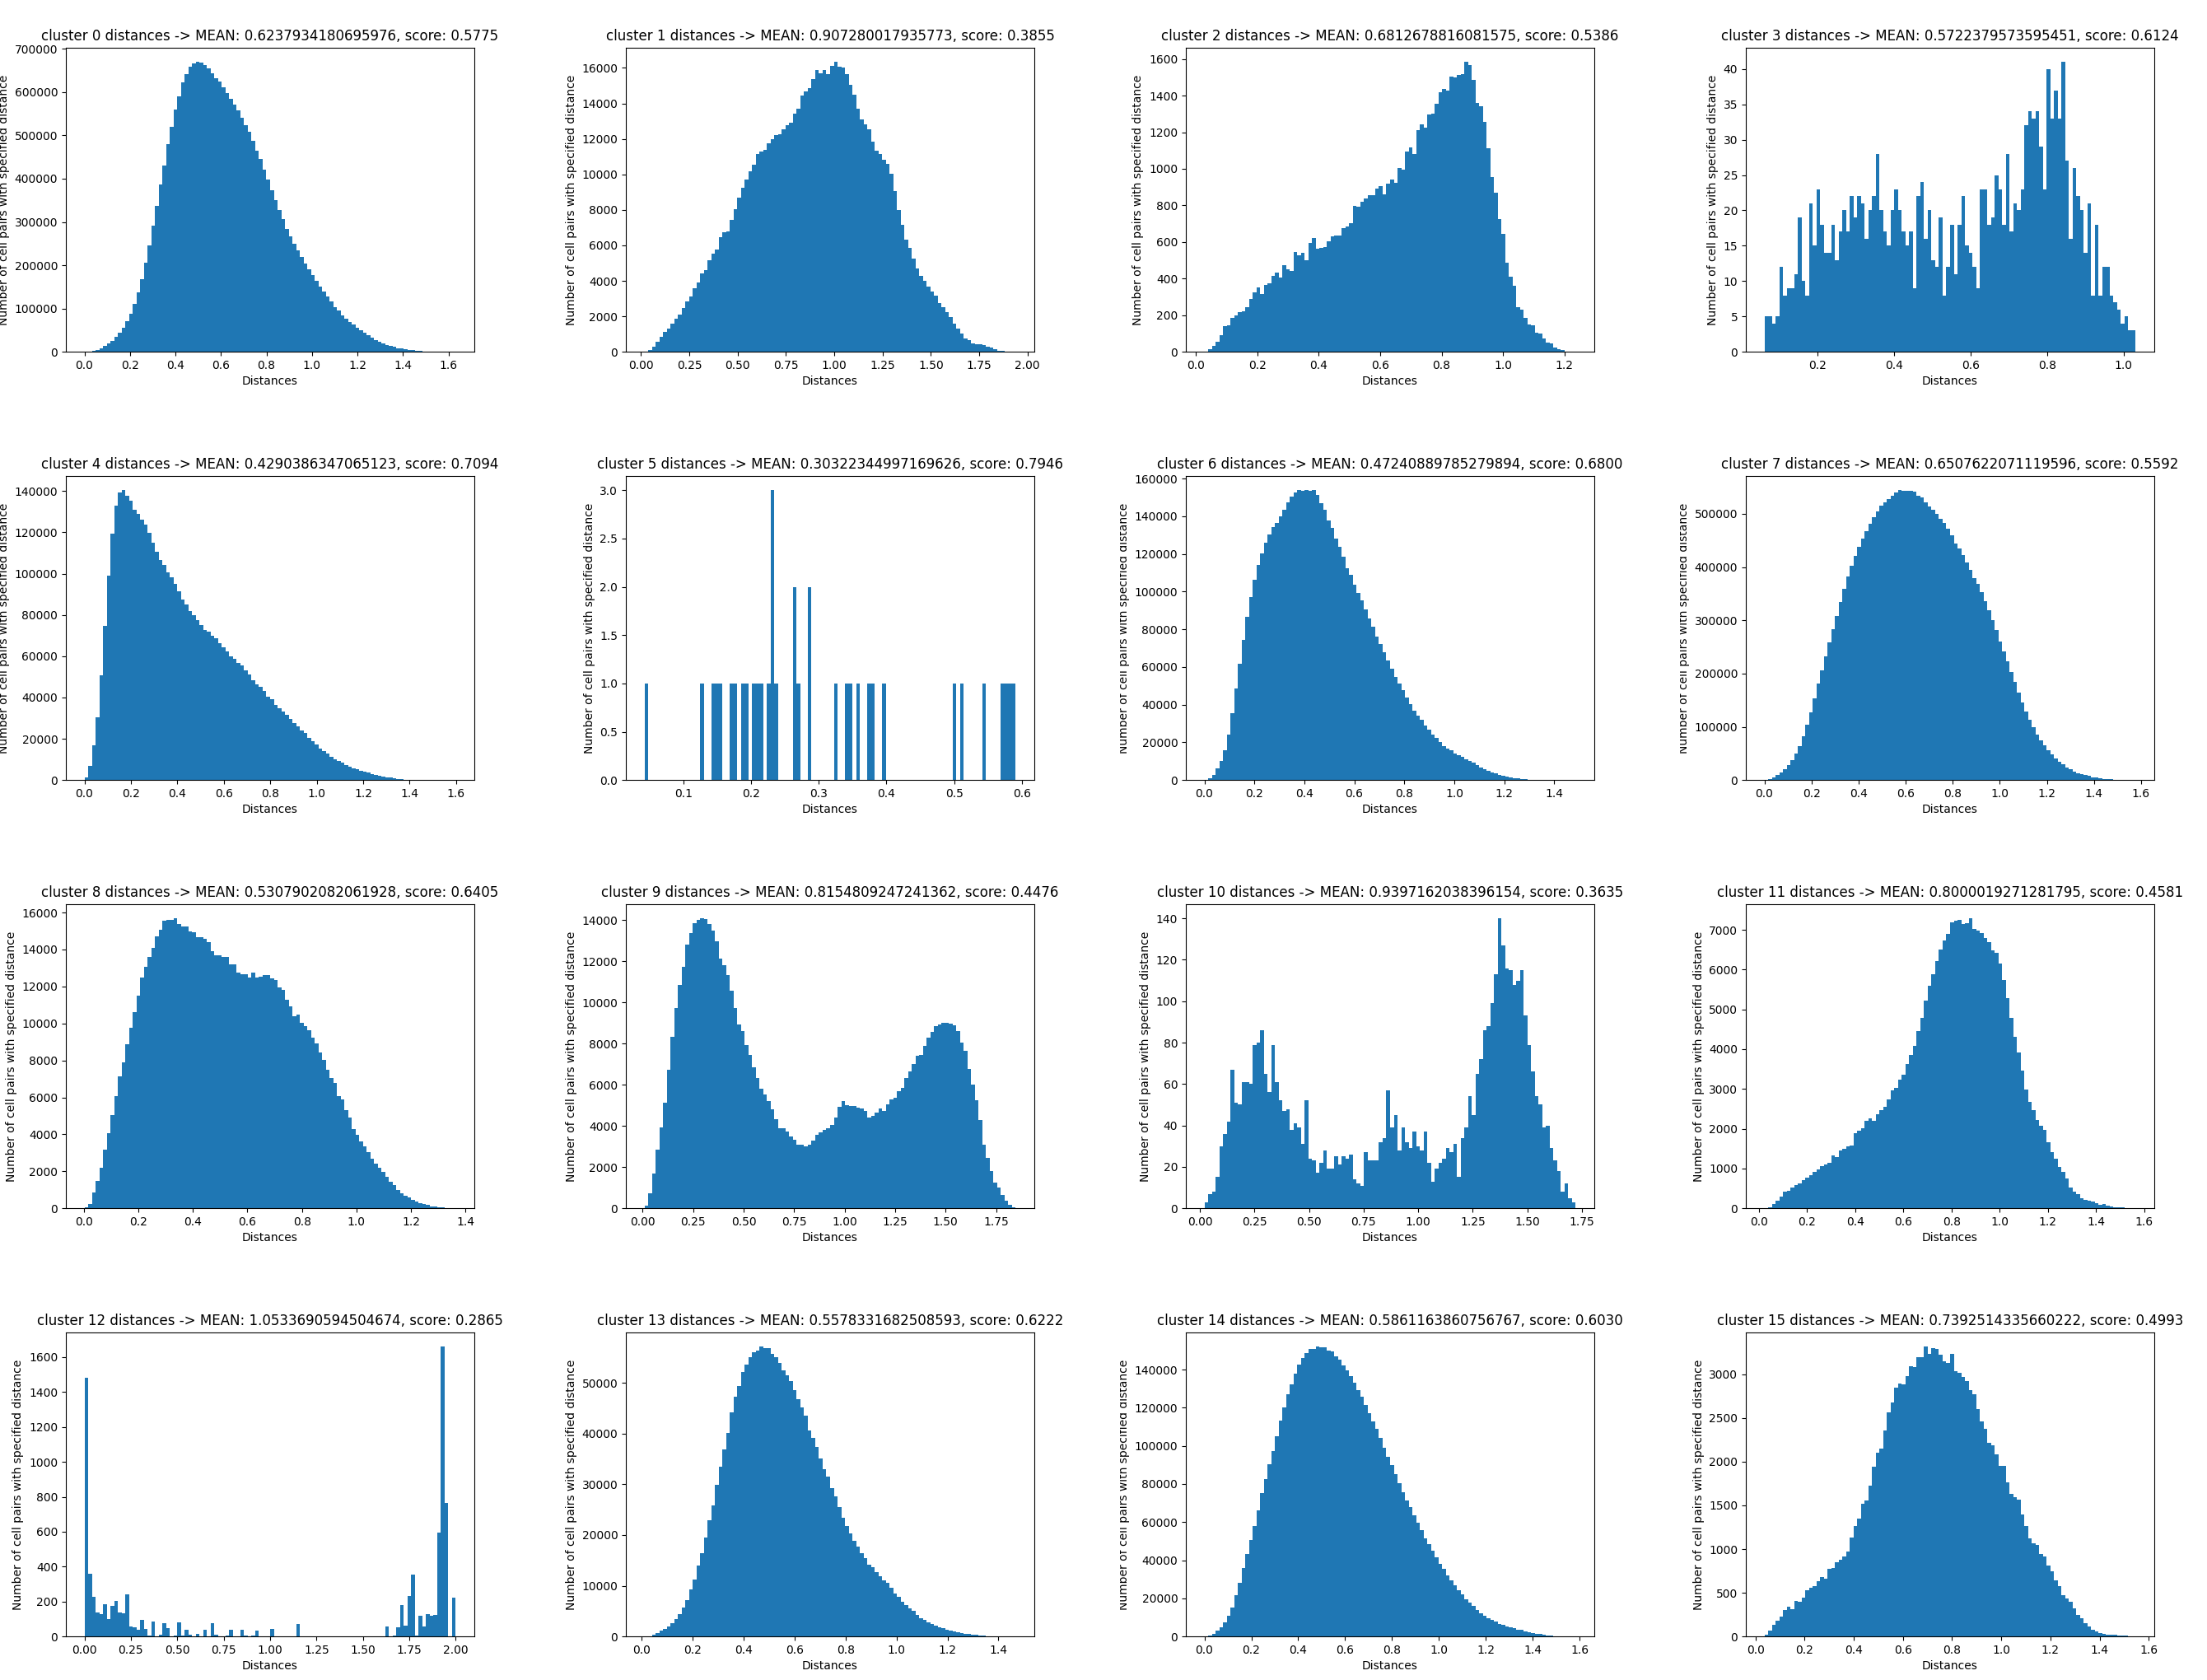
\includegraphics[width=0.8\textwidth]{stats_clusters3.png}
    \caption{Distribution of percentage distances between cells for each cluster}
\end{figure} 

\end{frame}

%%%%%%%%%%%%%%%%%%%%%%%%%%%%%%%%%%%%%%%%%%%%%%%%%%%%%%%%%%%%%%%%%%%%%%%%%%%%%%
\begin{frame}{Result 1 - Decreasing the threshold}

\begin{figure}
    \centering
    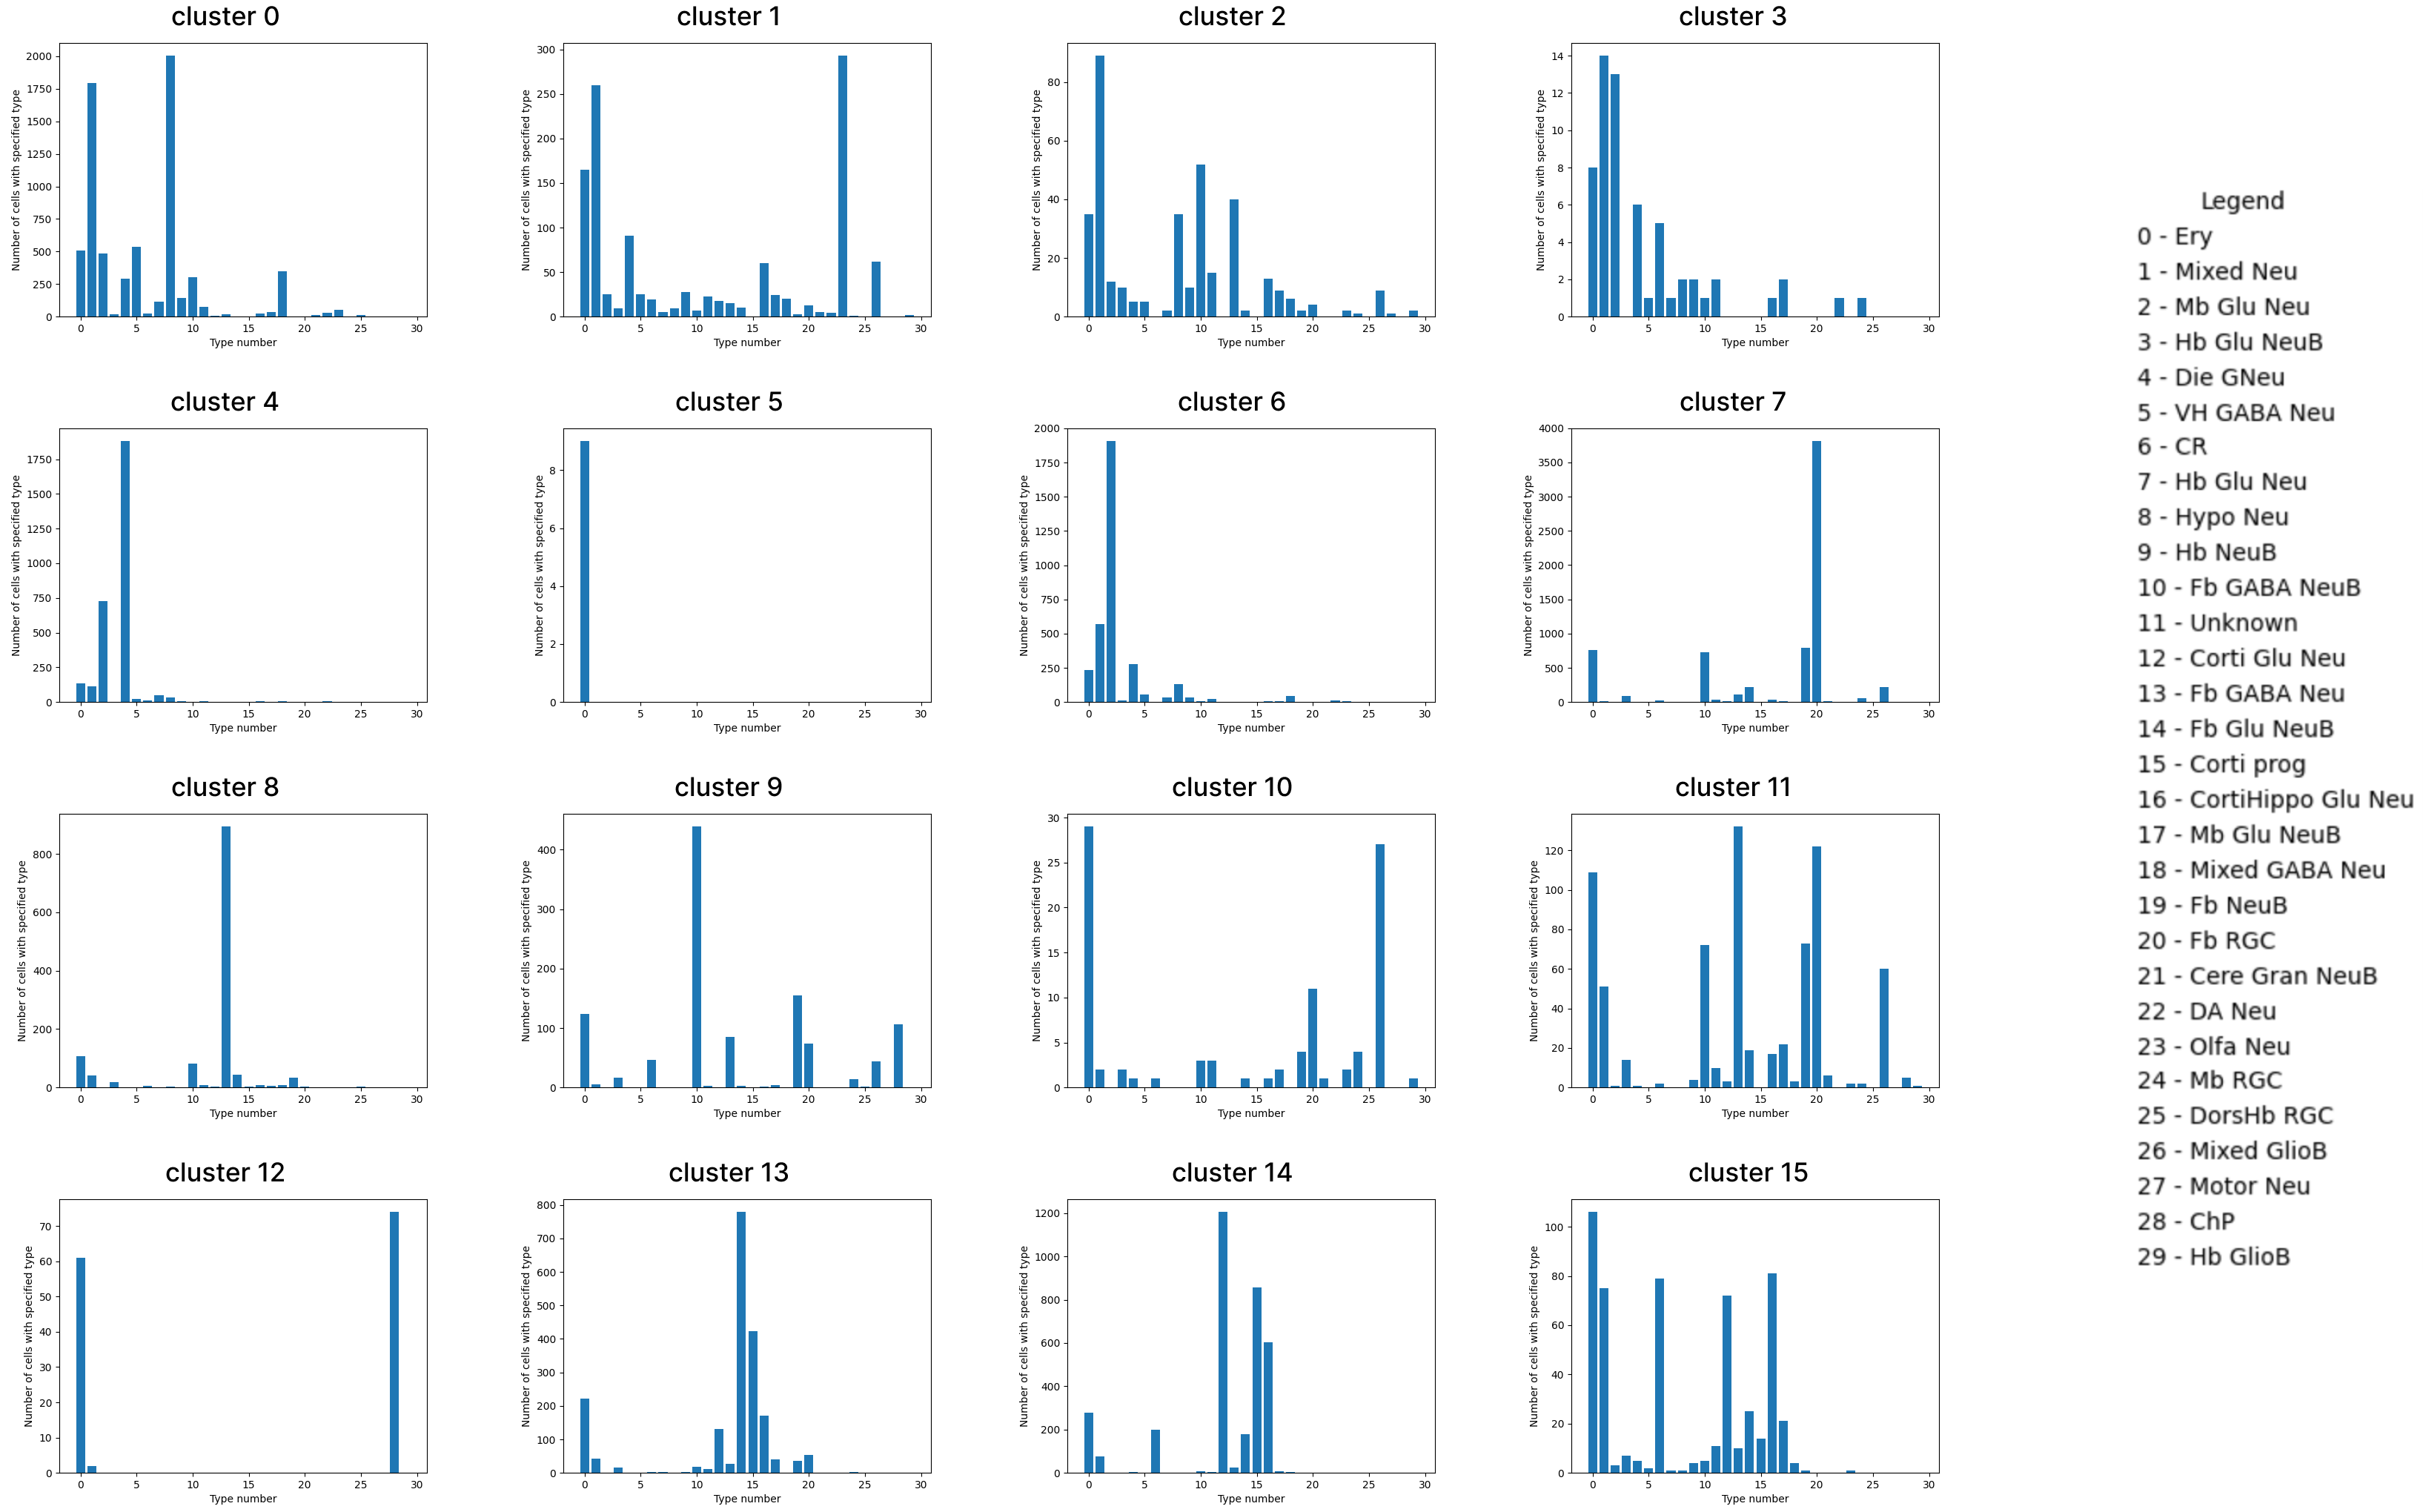
\includegraphics[width=0.8\textwidth]{type_num_clusters3.png}
    \caption{Number of different cell types in each cluster}
\end{figure} 

\end{frame}
%%%%%%%%%%%%%%%%%%%%%%%%%%%%%%%%%%%%%%%%%%%%%%%%%%%%%%%%%%%%%%%%%%%%%%%%%%%%%%
\begin{frame}{Result 1 - Decreasing the threshold}

\begin{figure}
    \centering
    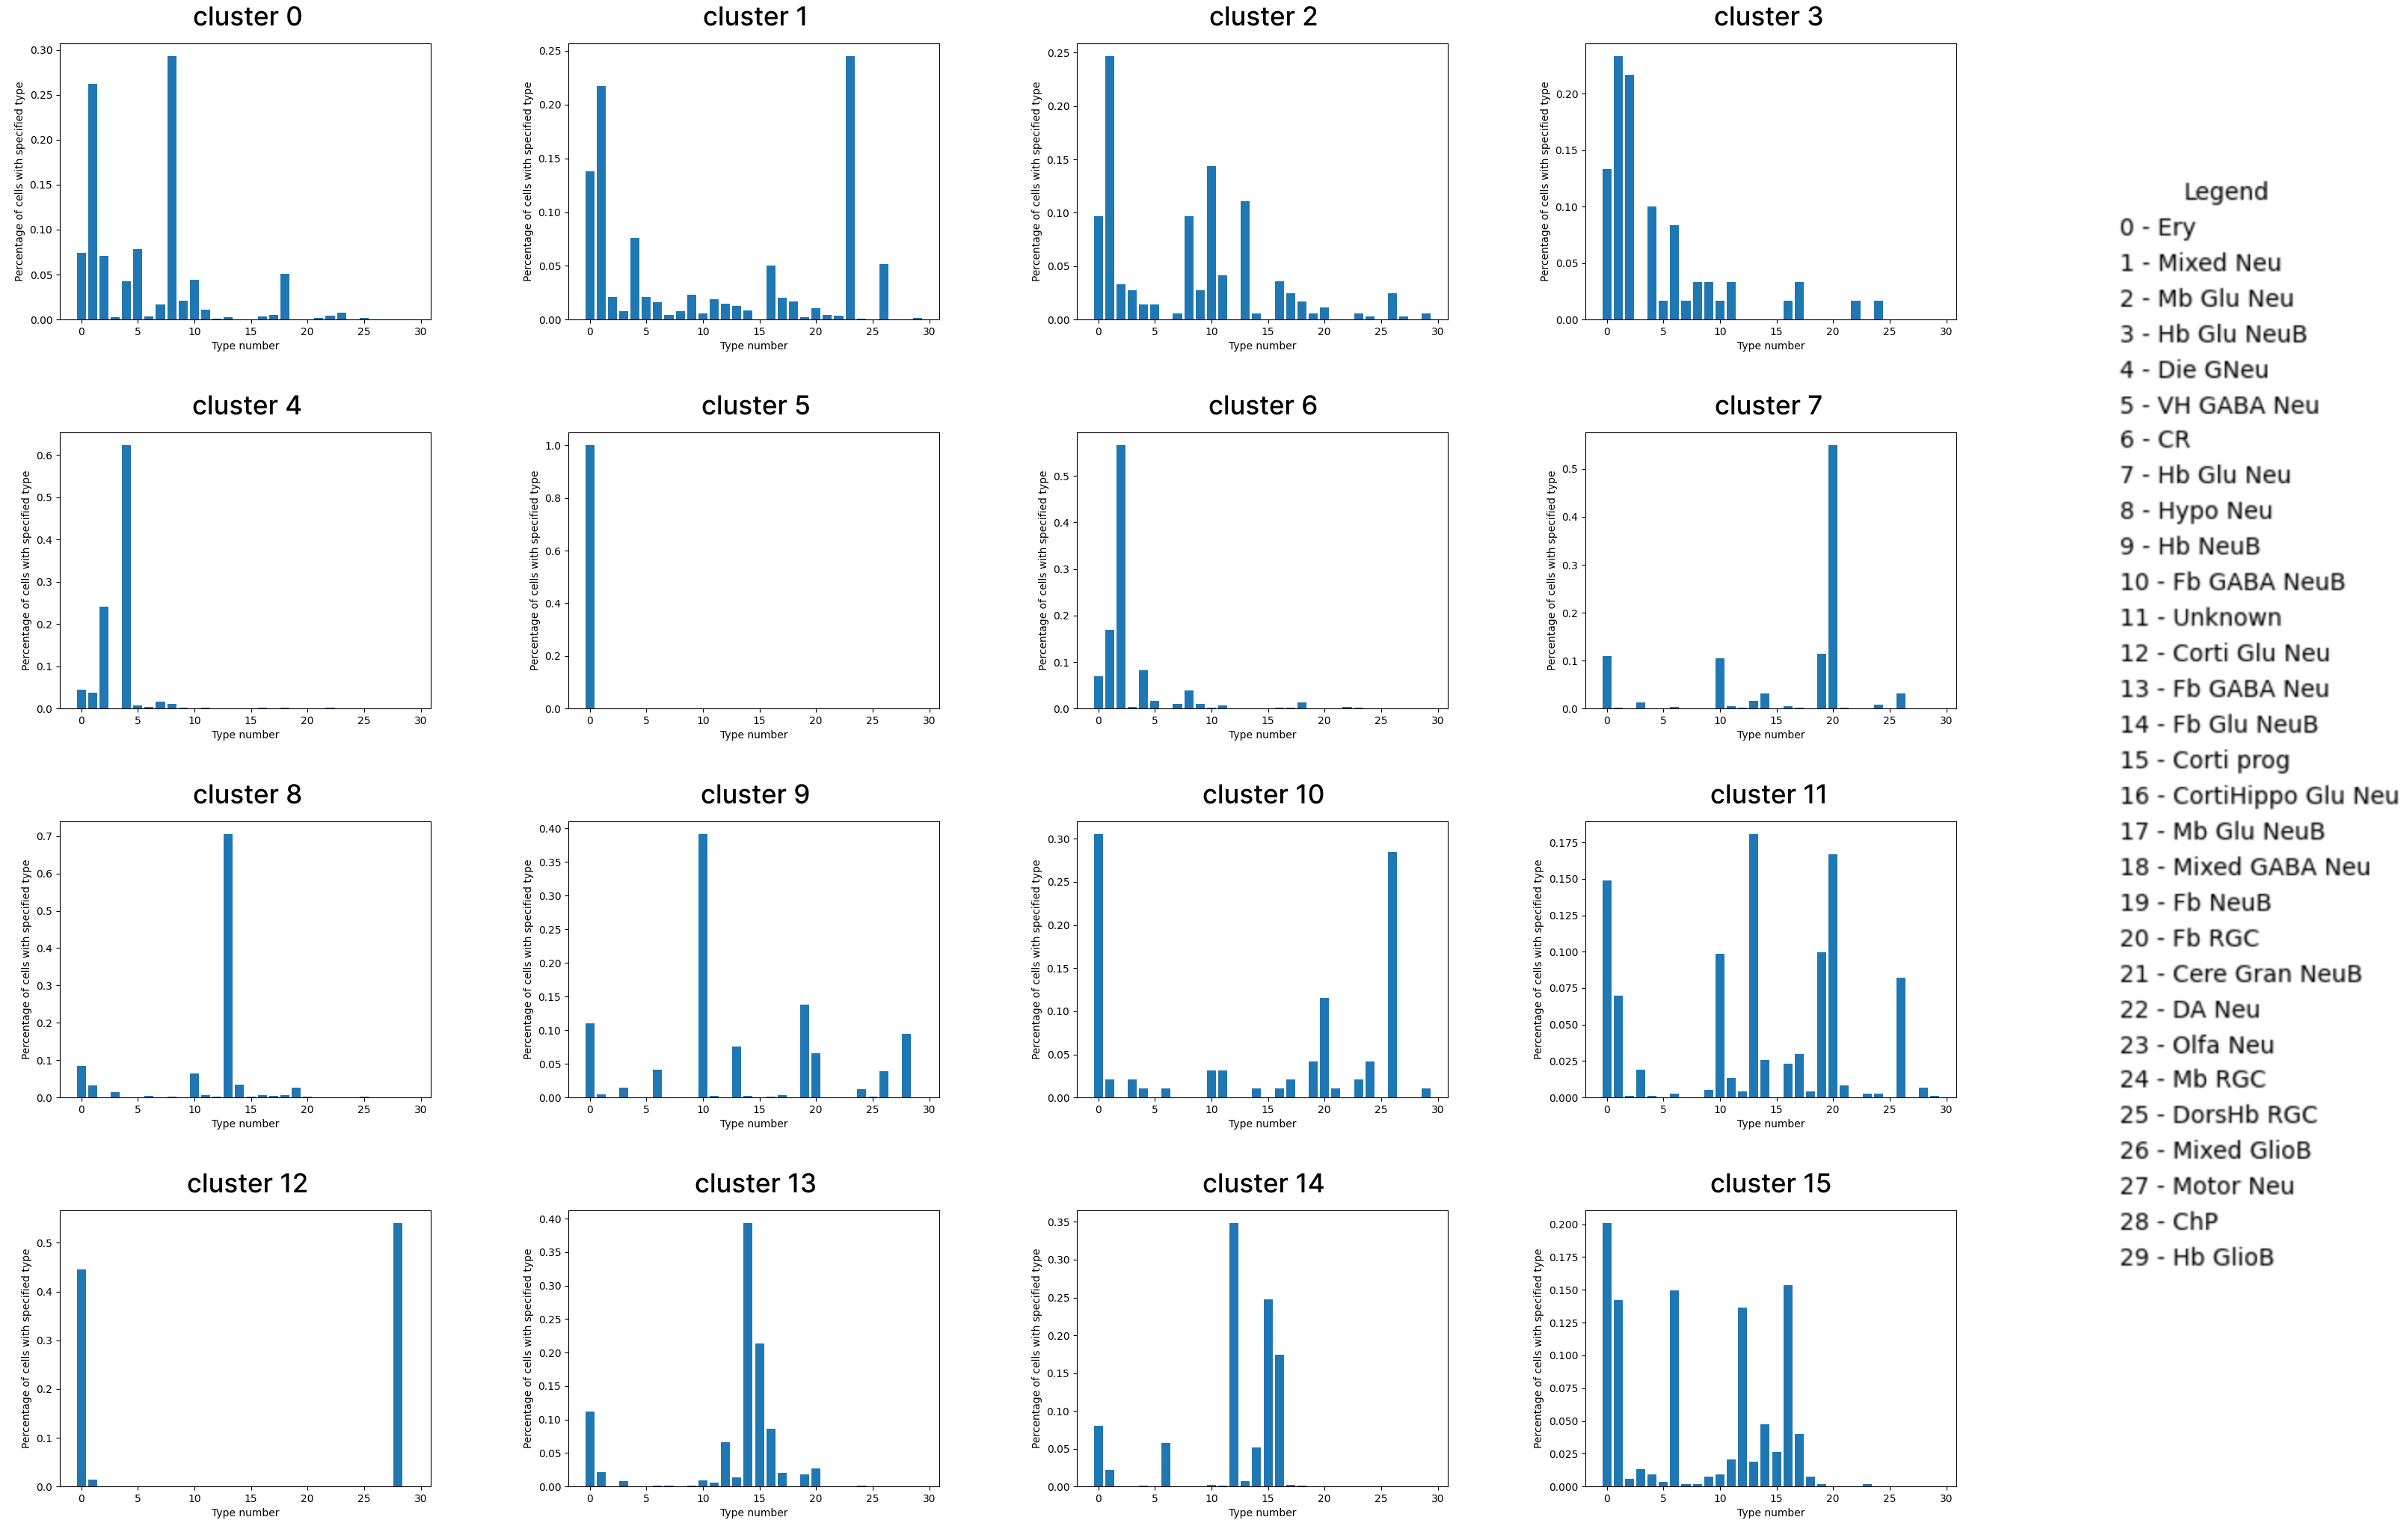
\includegraphics[width=0.8\textwidth]{type_p_clusters3.png}
    \caption{Percentage of different cell types in each cluster}
\end{figure} 

\end{frame}
%%%%%%%%%%%%%%%%%%%%%%%%%%%%%%%%%%%%%%%%%%%%%%%%%%%%%%%%%%%%%%%%%%%%%%%%%%%%%%
%%%%%%%%%%%%%%%%%%%%%%%%%%%%%%%%%%%%%%%%%%%%%%%%%%%%%%%%%%%%%%%%%%%%%%%%%%%%%%
%%%%%%%%%%%%%%%%%%%%%%%%%%%%%%%%%%%%%%%%%%%%%%%%%%%%%%%%%%%%%%%%%%%%%%%%%%%%%%
\begin{frame}{Result 1 - Decreasing the neighborhood radius}

\begin{itemize}
    \item<1-> []
    	\begin{figure}
   		 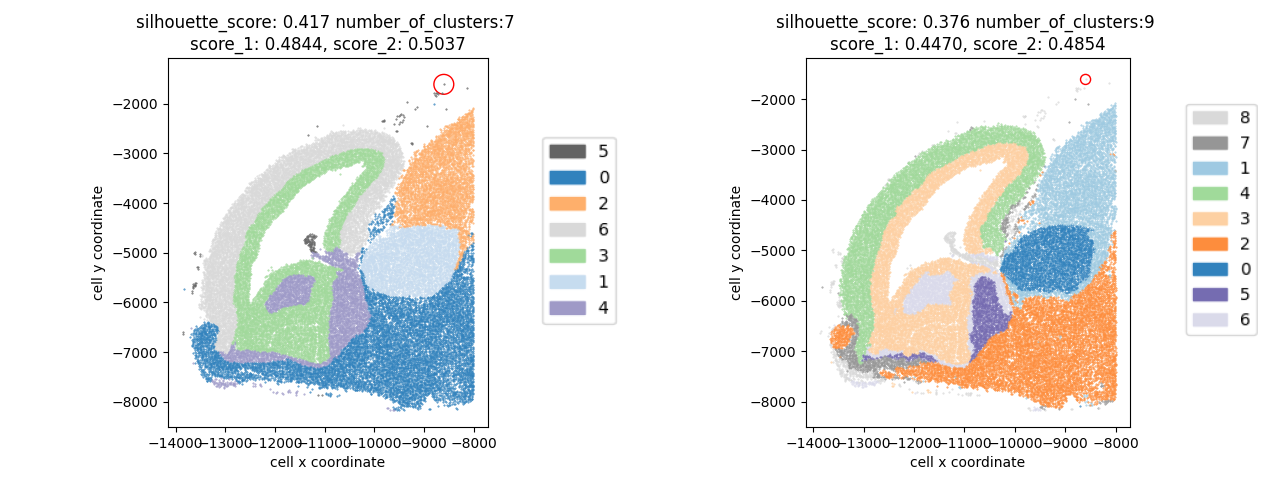
\includegraphics[width=0.7\textwidth]{clusters_1_3.png}
   		 \caption{Clusters with \texttt{neighborhood\_radius} $200$ and $100$, respectively}
	\end{figure} 
    \item<2-> Decreasing the neighborhood radius (from $200$ to $100$) did result in higher number of clusters, with a slightly lower silhouette and total homogeneity score. 
    \item <3-> The purple cluster (cluster $4$) from the previous clustering has now been divided into clusters $5$ and $6$ .This division has resulted in higher homogeneity scores for clusters $5$ ($0.59$) and $6$ ($0.36$) than what was observed for the single cluster $4$ ($0.26$) in the previous clustering. 
\end{itemize}

\end{frame}

%%%%%%%%%%%%%%%%%%%%%%%%%%%%%%%%%%%%%%%%%%%%%%%%%%%%%%%%%%%%%%%%%%%%%%%%%%%%%%
\begin{frame}{Result 1 - Decreasing the neighborhood radius}
\begin{itemize}
   \item<1-> []
   	\begin{figure}
   	 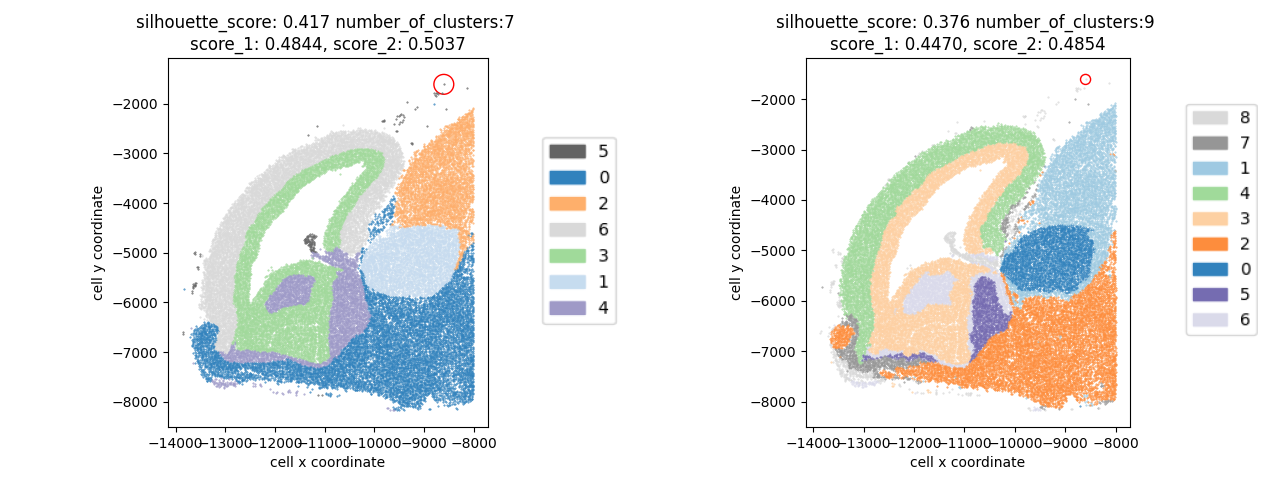
\includegraphics[width=0.55\textwidth]{clusters_1_3.png}
  	  \caption{Clusters with \texttt{neighborhood\_radius} $200$ and $100$, respectively}
	\end{figure} 
    \item<2->  The blue cluster (cluster $0$) from the previous clustering has now been divided into clusters $2$ and $7$.This division has resulted in higher homogeneity scores for cluster $2$ ($0.47$) and lower for cluster $7$ ($0.3$) than what was observed for the single cluster $0$ ($0.45$) in the previous clustering. 
    \item<3->  The green cluster (cluster $3$) from the previous clustering ($0.56$) has slightly higher homogeneity scores than cluster $3$ in new clustering ($0.51$), same as clusters $6$ from the previous clustering ($0.45$) and cluster $4$ from the new clustering ($0.37$).
\end{itemize}

\end{frame}
%%%%%%%%%%%%%%%%%%%%%%%%%%%%%%%%%%%%%%%%%%%%%%%%%%%%%%%%%%%%%%%%%%%%%%%%%%%%%%

\begin{frame}{Result 1 - Decreasing the neighborhood radius}

\begin{itemize}
    \item<1-> The mean of distribution of percentage distances between all cells is $1.58$, as shown in the image below
    \begin{figure}
    \centering
    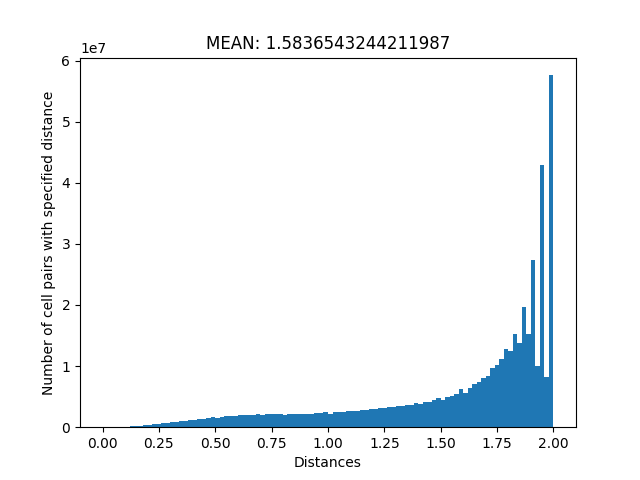
\includegraphics[width=0.7\textwidth]{all_distances2_1.png}
    \caption{Distribution of percentage distances between all cells}
\end{figure} 
   
\end{itemize}
\end{frame}
%%%%%%%%%%%%%%%%%%%%%%%%%%%%%%%%%%%%%%%%%%%%%%%%%%%%%%%%%%%%%%%%%%%%%%%%%%%%%%
\begin{frame}{Result 1 - Decreasing the neighborhood radius}

\begin{figure}
    \centering
    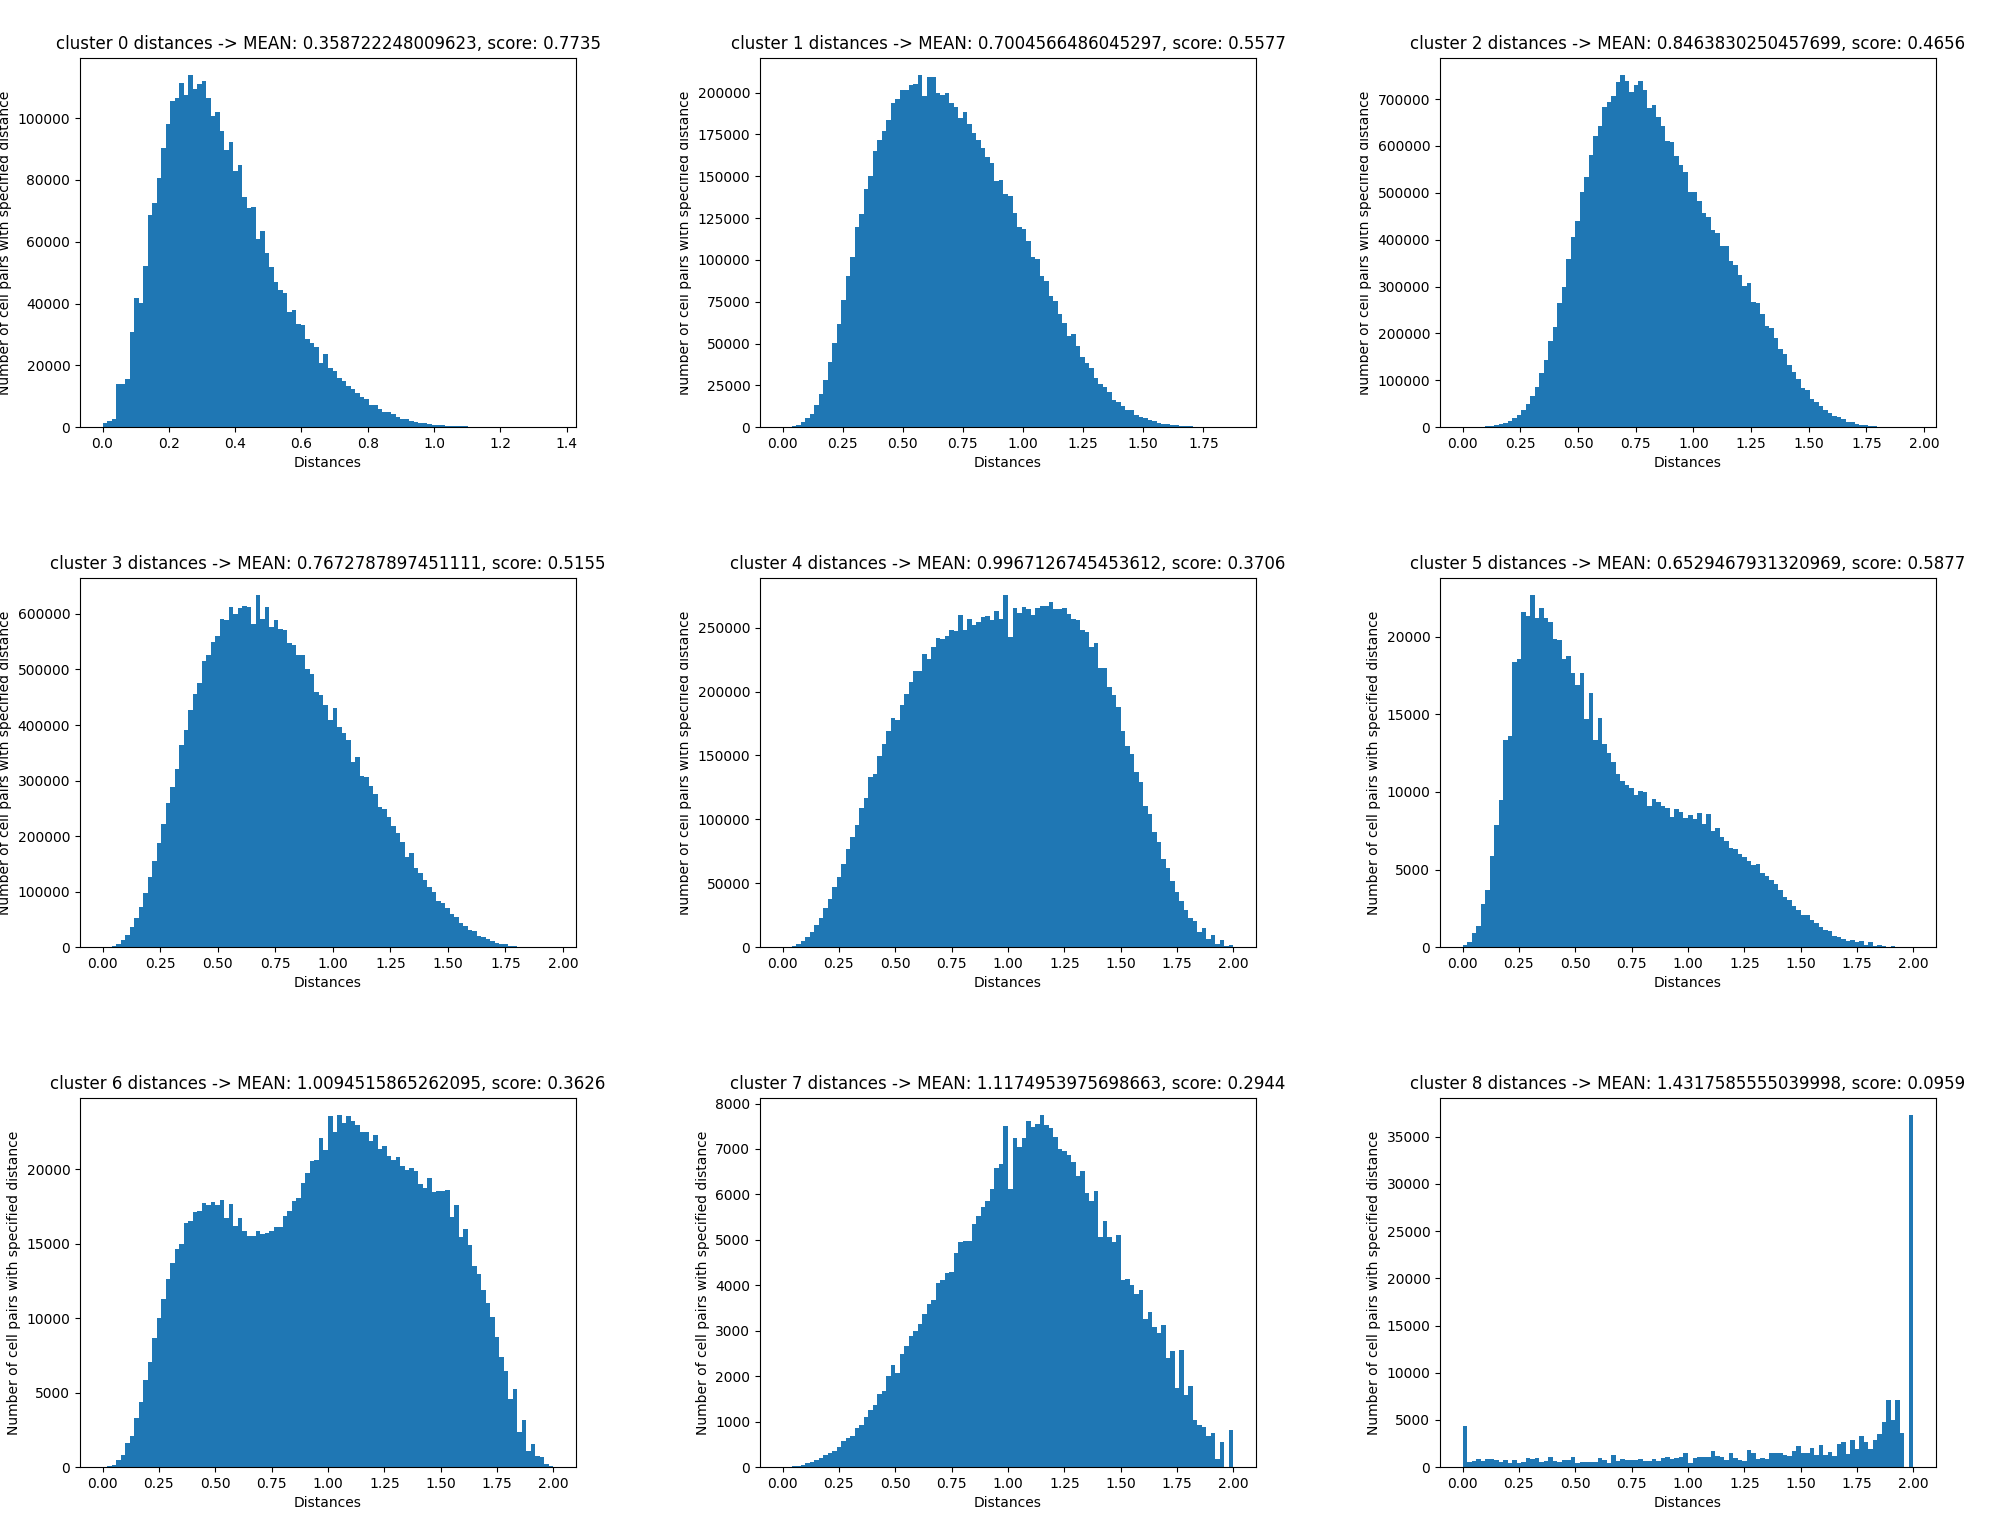
\includegraphics[width=0.8\textwidth]{stats_clusters1.png}
    \caption{Distribution of percentage distances between cells for each cluster}
\end{figure} 

\end{frame}
%%%%%%%%%%%%%%%%%%%%%%%%%%%%%%%%%%%%%%%%%%%%%%%%%%%%%%%%%%%%%%%%%%%%%%%%%%%%%%










%%%%%%%%%%%%%%%%%%%%%%%%%%%%%%%%%%%%%%%%%%%%%%%%%%%%%%%%%%%%%%%%%%%%%%%%%%%%%%%
%%%%%%%%%%%%%%%%%%%%%%%%%%%%%%%%%%%%%%%%%%%%%%%%%%%%%%%%%%%%%%%%%%%%%%%%%%%%%%
\begin{frame}{Result 2}

\begin{itemize}
    \item<1-> Results where:
    \begin{itemize}
        \item<2-> \texttt{neighborhood\_radius = 200} (the radius that corresponds to the red circle in the image below)
        \item<3-> \texttt{distance\_function = Euclidean}
        \item<4-> \texttt{linkage\_method = centroid}
    \end{itemize}
    \item<5-> []
    	\begin{figure}
		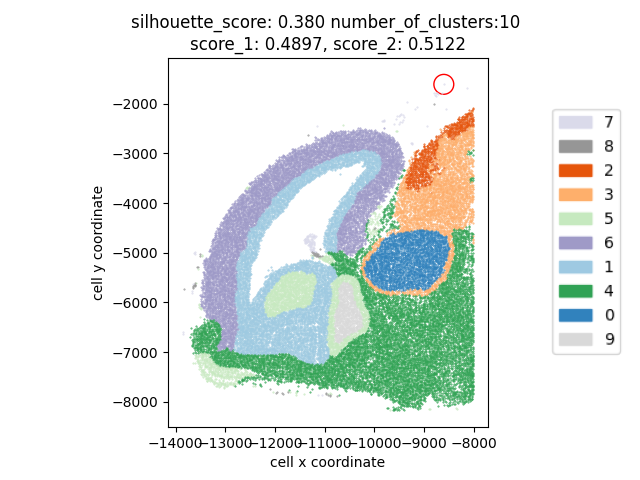
\includegraphics[width=0.55\textwidth]{clusters_4.png}
    		\caption{Clusters}
	\end{figure} 
\end{itemize}



\end{frame}
%%%%%%%%%%%%%%%%%%%%%%%%%%%%%%%%%%%%%%%%%%%%%%%%%%%%%%%%%%%%%%%%%%%%%%%%%%%%%%
\begin{frame}{Result 2 - Statistics of clusters}

\begin{itemize}
    \item<1-> The mean of distribution of percentage distances between all cells is $0.63$, as shown in the image below
    \begin{figure}
    \centering
    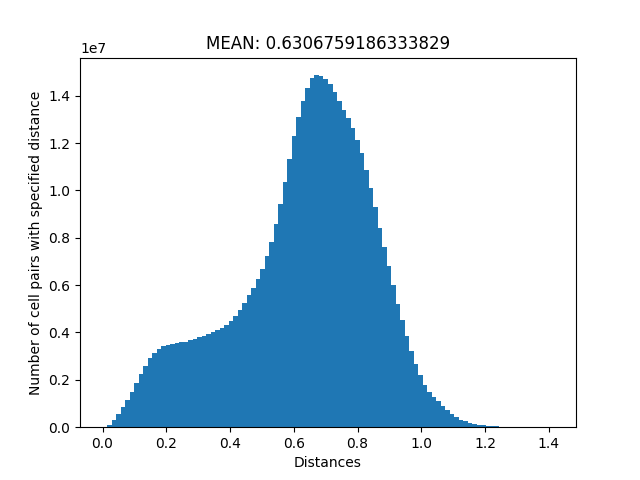
\includegraphics[width=0.6\textwidth]{all_distances4.png}
    \caption{Distribution of percentage distances between all cells}
\end{figure} 
   
\end{itemize}
\end{frame}
%%%%%%%%%%%%%%%%%%%%%%%%%%%%%%%%%%%%%%%%%%%%%%%%%%%%%%%%%%%%%%%%%%%%%%%%%%%%%%
\begin{frame}{Result 2 - Homogeneous or Heterogeneous clusters}

\begin{figure}
    \centering
    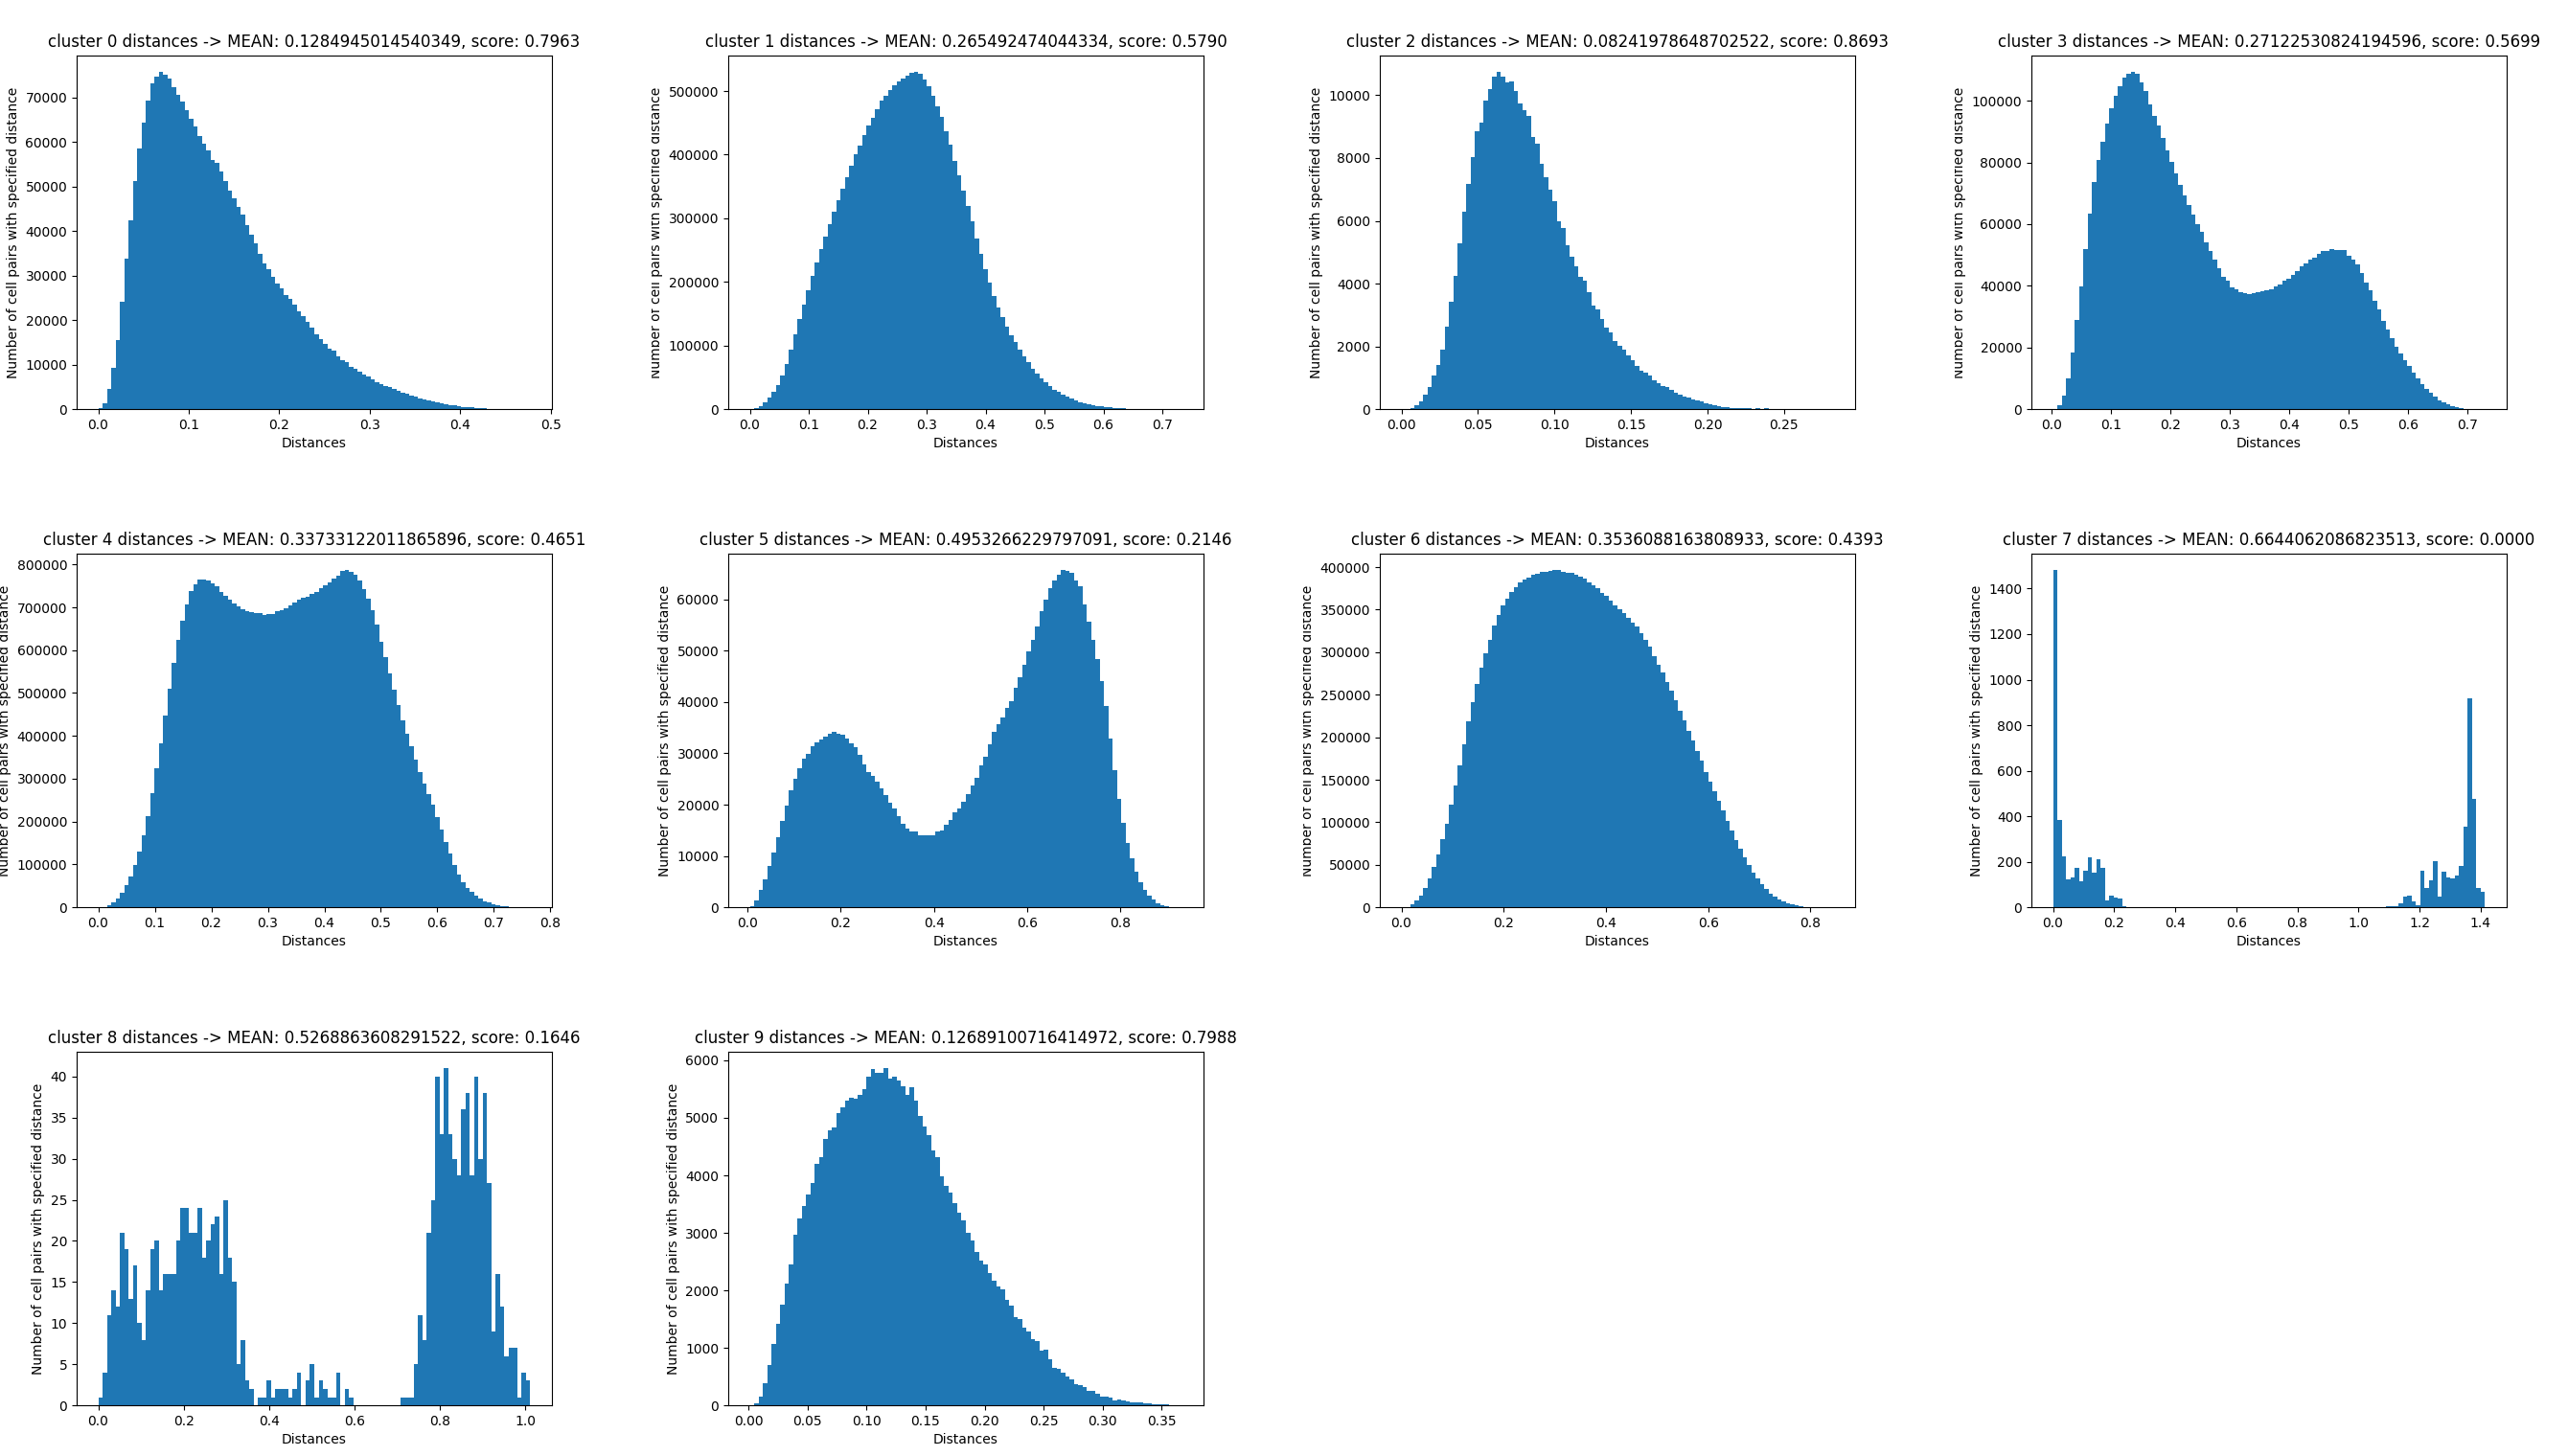
\includegraphics[width=1\textwidth]{stats_clusters4.png}
    \caption{Distribution of percentage distances between cells for each cluster}
\end{figure} 

\end{frame}
%%%%%%%%%%%%%%%%%%%%%%%%%%%%%%%%%%%%%%%%%%%%%%%%%%%%%%%%%%%%%%%%%%%%%%%%%%%%%%
\begin{frame}{Result 2 - Homogeneous or Heterogeneous clusters}

\begin{itemize}
    \item<1->  As observed in the image above, there are distributions, particularly for clusters $5$, $7$, and $8$, which may suggest that these clusters need to be divided or that this clustering isn't optimal
    \item<2->  Furthermore, clusters $7$ and $8$ contain the smallest number of cells, with cluster $8$ having low cell count (shown in the image below)
    \item<3->  Distributions for the other clusters are more promising. Cluster $0$, $1$, $2$, $3$ and $9$ are homogeneous and clusters $4$ and $6$ are close to homogeneous
    \item<4->  Total homogeneity score of this clustering is $0.51$ and silhouette score is $0.38$
\end{itemize}
\end{frame}

%%%%%%%%%%%%%%%%%%%%%%%%%%%%%%%%%%%%%%%%%%%%%%%%%%%%%%%%%%%%%%%%%%%%%%%%%%%%%%
\begin{frame}{Result 2 - Number of different cell types in each cluster}

\begin{figure}
    \centering
    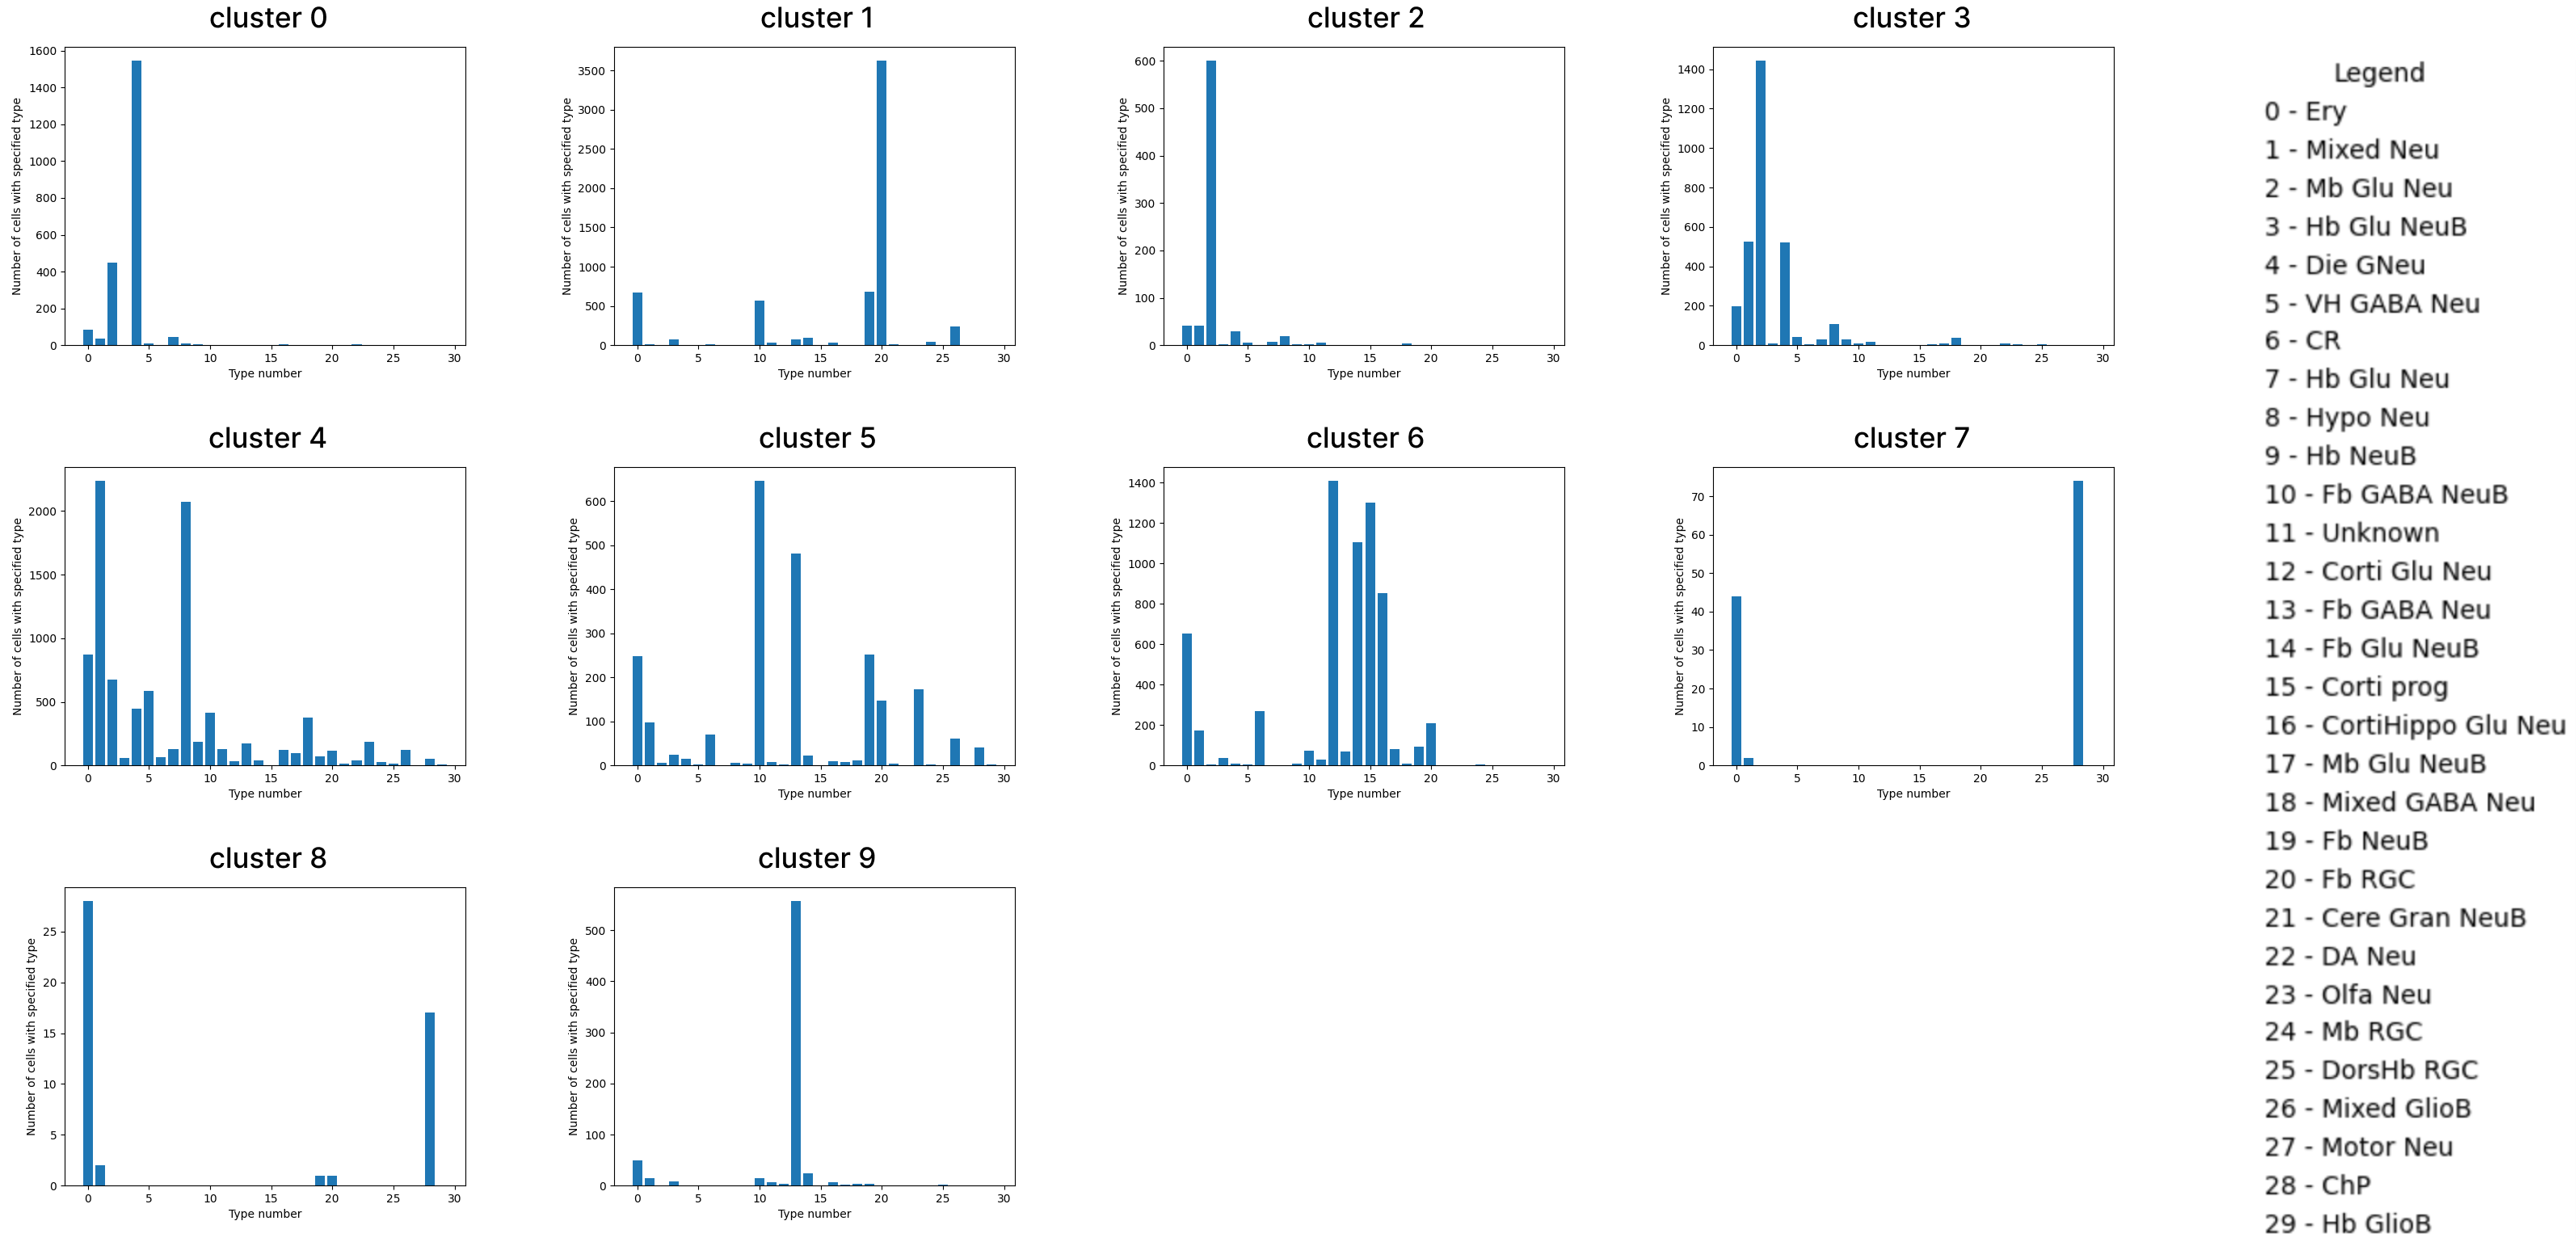
\includegraphics[width=1\textwidth]{type_num_clusters4.png}
    \caption{Number of different cell types in each cluster}
\end{figure} 

\end{frame}
%%%%%%%%%%%%%%%%%%%%%%%%%%%%%%%%%%%%%%%%%%%%%%%%%%%%%%%%%%%%%%%%%%%%%%%%%%%%%%
\begin{frame}{Result 2 - Percentage of different cell types in each cluster}

\begin{figure}
    \centering
    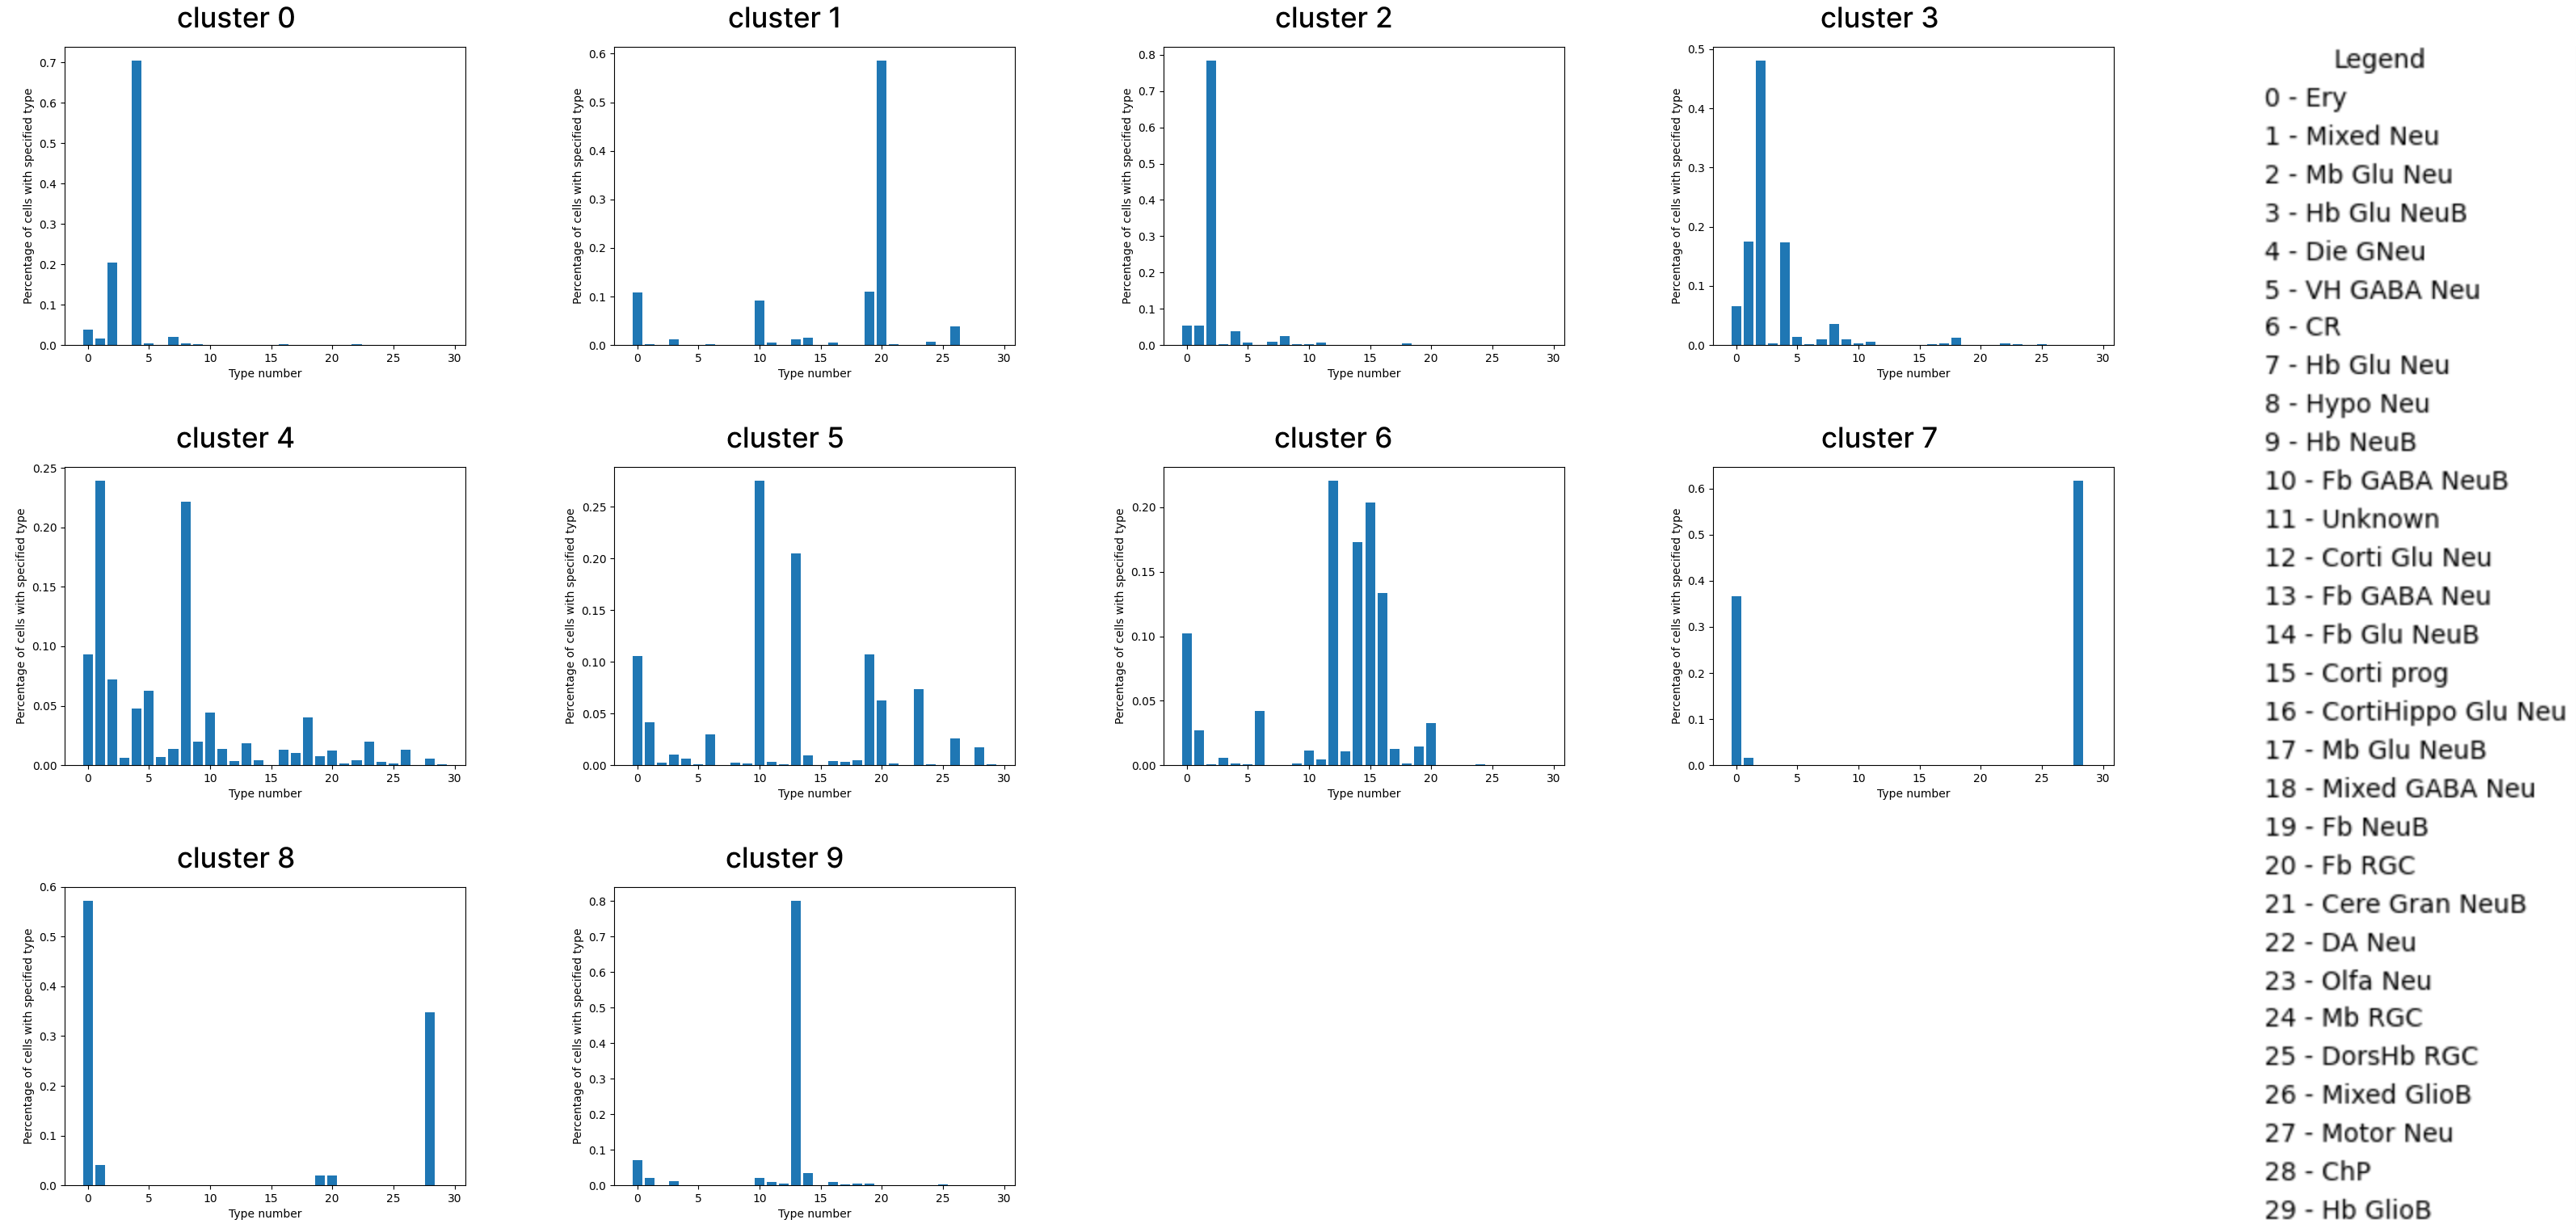
\includegraphics[width=1\textwidth]{type_p_clusters4.png}
    \caption{Percentage of different cell types in each cluster}
\end{figure} 

\end{frame}
%%%%%%%%%%%%%%%%%%%%%%%%%%%%%%%%%%%%%%%%%%%%%%%%%%%%%%%%%%%%%%%%%%%%%%%%%%%%%%
%%%%%%%%%%%%%%%%%%%%%%%%%%%%%%%%%%%%%%%%%%%%%%%%%%%%%%%%%%%%%%%%%%%%%%%%%%%%%%





%%%%%%%%%%%%%%%%%%%%%%%%%%%%%%%%%%%%%%%%%%%%%%%%%%%%%%%%%%%%%%%%%%%%%%%%%%%%%%%
%%%%%%%%%%%%%%%%%%%%%%%%%%%%%%%%%%%%%%%%%%%%%%%%%%%%%%%%%%%%%%%%%%%%%%%%%%%%%%
\begin{frame}{Result 3}

\begin{itemize}
    \item<1->  Results where:
    \begin{itemize}
        \item<2->  \texttt{neighborhood\_radius = 150} (the radius that corresponds to the red circle in the image below)
        \item<3->  \texttt{distance\_function = Hamming} with \texttt{hamming\_param = 0.3}
        \item<4->  \texttt{linkage\_method = average}
        \item<5->  \texttt{threshold = 30}
        \item<6-> []
        \begin{figure}
   		 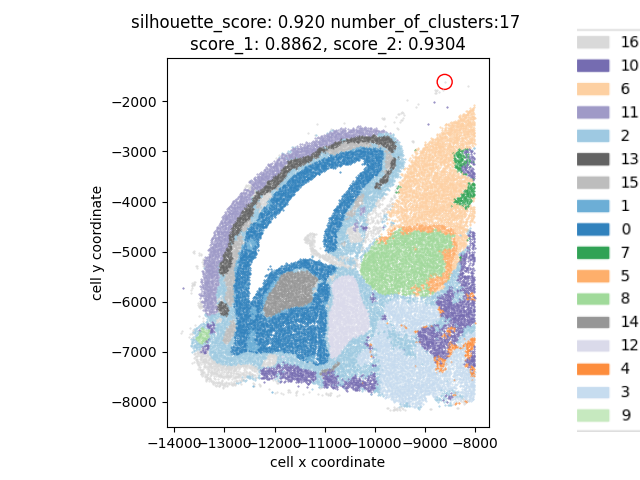
\includegraphics[width=0.55\textwidth]{clusters_5.png}
    		\caption{Clusters}
	\end{figure} 
    \end{itemize}
\end{itemize}

\end{frame}
%%%%%%%%%%%%%%%%%%%%%%%%%%%%%%%%%%%%%%%%%%%%%%%%%%%%%%%%%%%%%%%%%%%%%%%%%%%%%%
\begin{frame}{Result 3 - Statistics of clusters}

\begin{itemize}
    \item<1-> The mean of distribution of percentage distances between all cells is $0.89$, as shown in the image below
    \begin{figure}
    \centering
    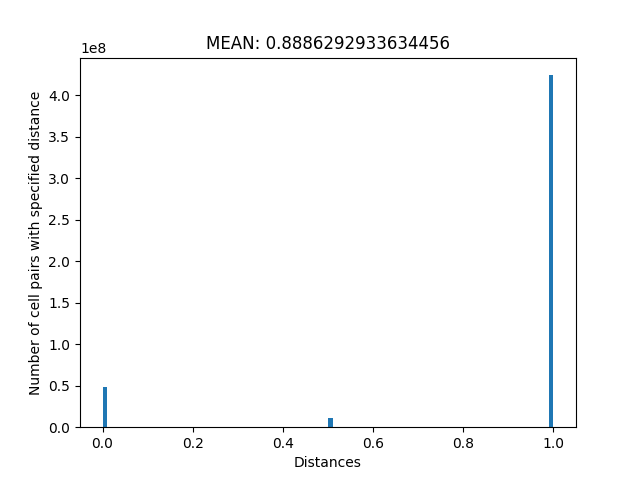
\includegraphics[width=0.55\textwidth]{all_distances5.png}
    \caption{Distribution of percentage distances between all cells}
\end{figure} 
   
\end{itemize}
\end{frame}
%%%%%%%%%%%%%%%%%%%%%%%%%%%%%%%%%%%%%%%%%%%%%%%%%%%%%%%%%%%%%%%%%%%%%%%%%%%%%%
\begin{frame}{Result 3 - Homogeneous or Heterogeneous clusters}

\begin{figure}
    \centering
    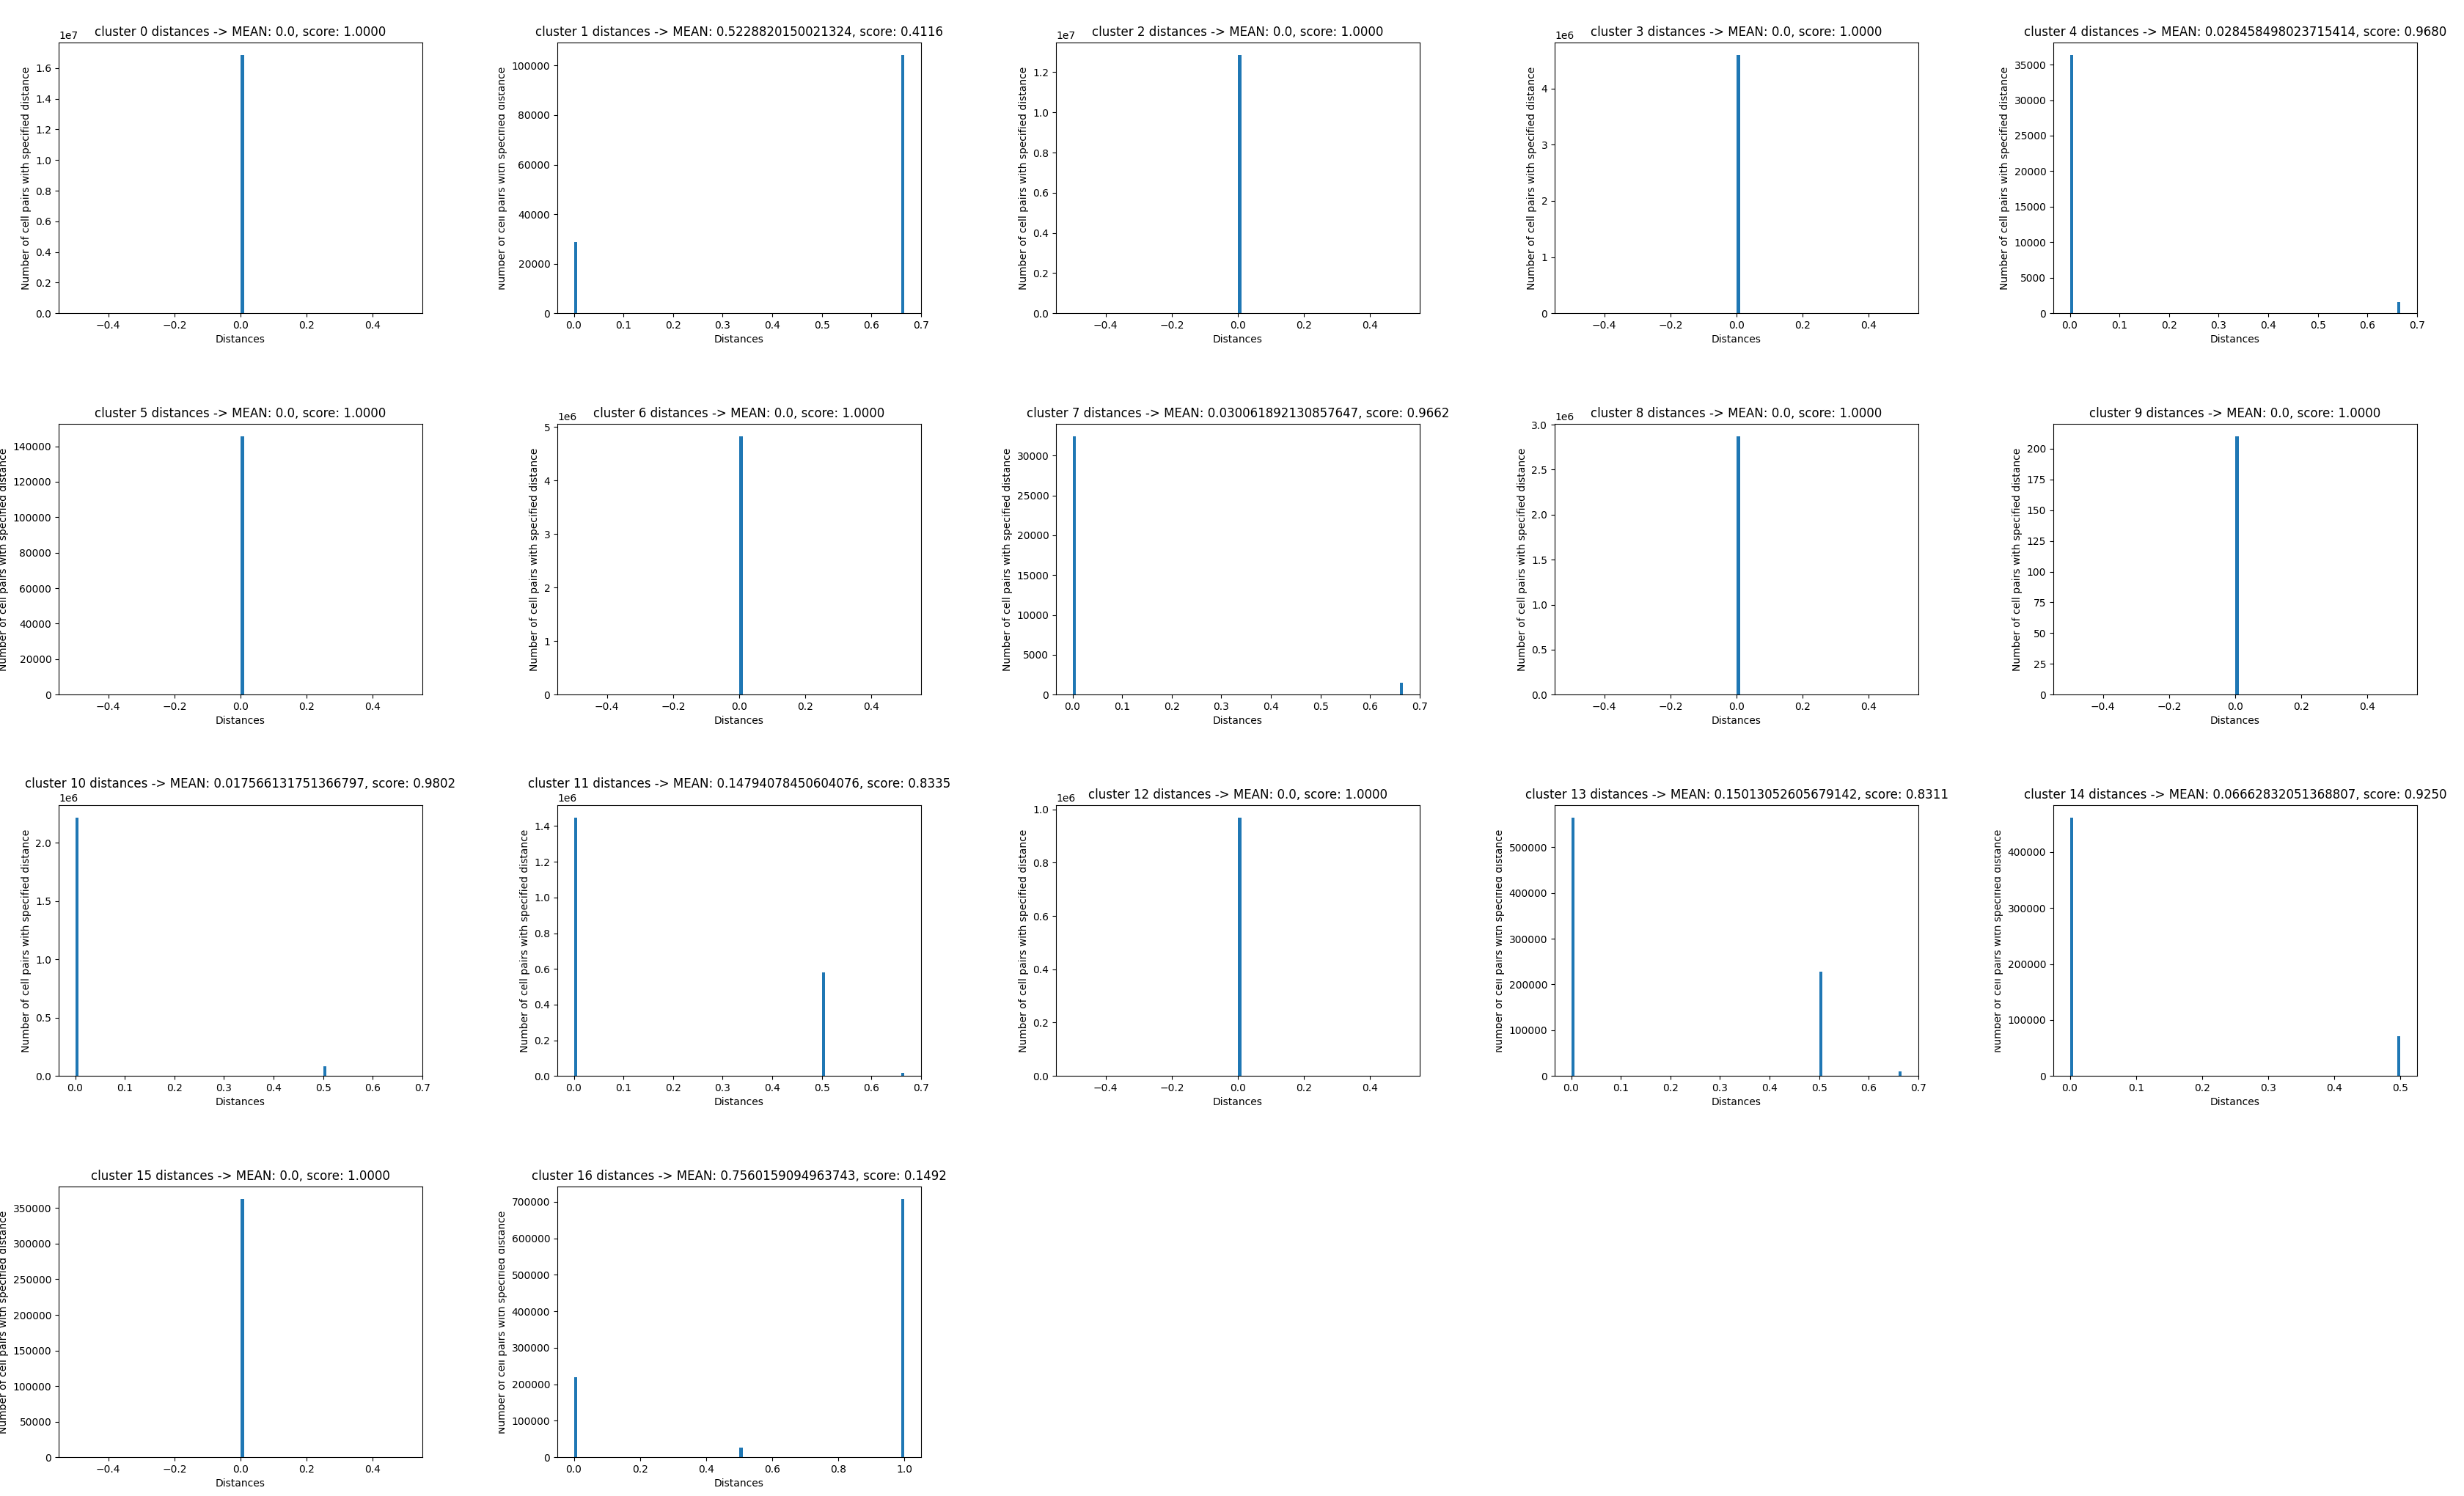
\includegraphics[width=1\textwidth]{stats_clusters5.png}
    \caption{Distribution of percentage distances between cells for each cluster}
\end{figure} 

\end{frame}
%%%%%%%%%%%%%%%%%%%%%%%%%%%%%%%%%%%%%%%%%%%%%%%%%%%%%%%%%%%%%%%%%%%%%%%%%%%%%%
\begin{frame}{Result 3 - Homogeneous or Heterogeneous clusters}

\begin{itemize}
    \item<1-> From the image above, all clusters, except clusters $1$ and $16$, are homogeneous with high homogeneity scores
    \item<2-> Total homogeneity score of this clustering is $0.93$ and silhouette score is $0.92$
\end{itemize}
\end{frame}

%%%%%%%%%%%%%%%%%%%%%%%%%%%%%%%%%%%%%%%%%%%%%%%%%%%%%%%%%%%%%%%%%%%%%%%%%%%%%%
\begin{frame}{Result 3 - Number of different cell types in each cluster}

\begin{figure}
    \centering
    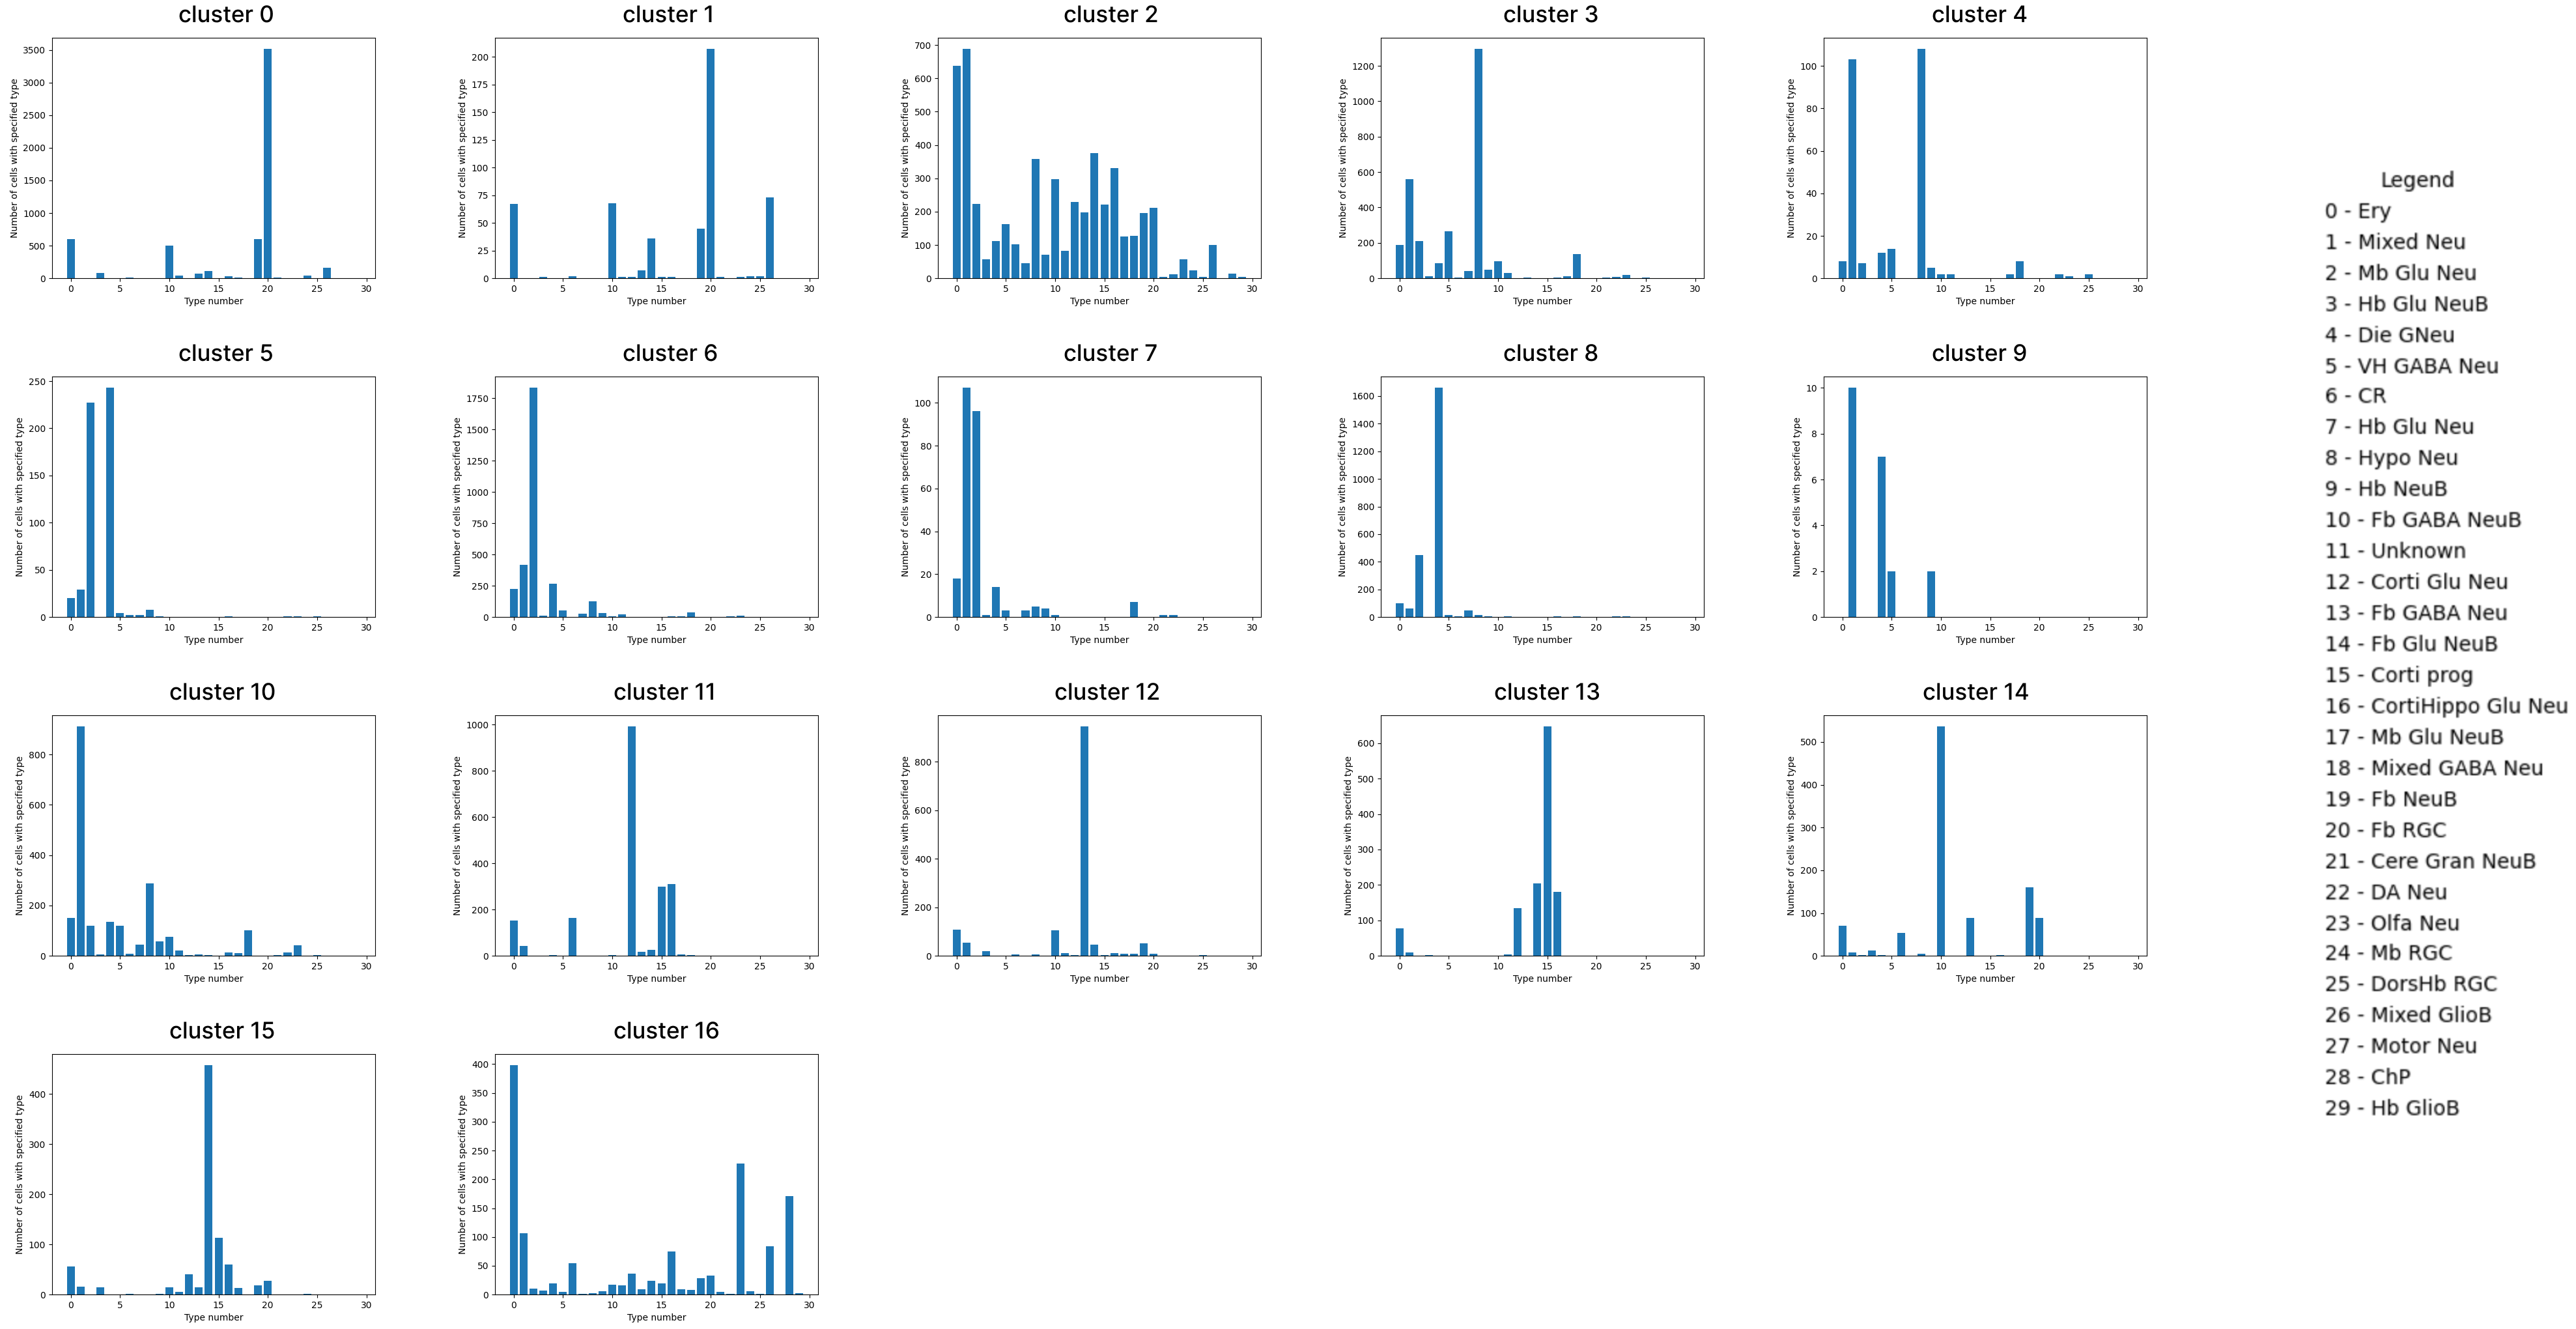
\includegraphics[width=1\textwidth]{type_num_clusters5.png}
    \caption{Number of different cell types in each cluster}
\end{figure} 

\end{frame}
%%%%%%%%%%%%%%%%%%%%%%%%%%%%%%%%%%%%%%%%%%%%%%%%%%%%%%%%%%%%%%%%%%%%%%%%%%%%%%
\begin{frame}{Result 3 - Percentage of different cell types in each cluster}

\begin{figure}
    \centering
    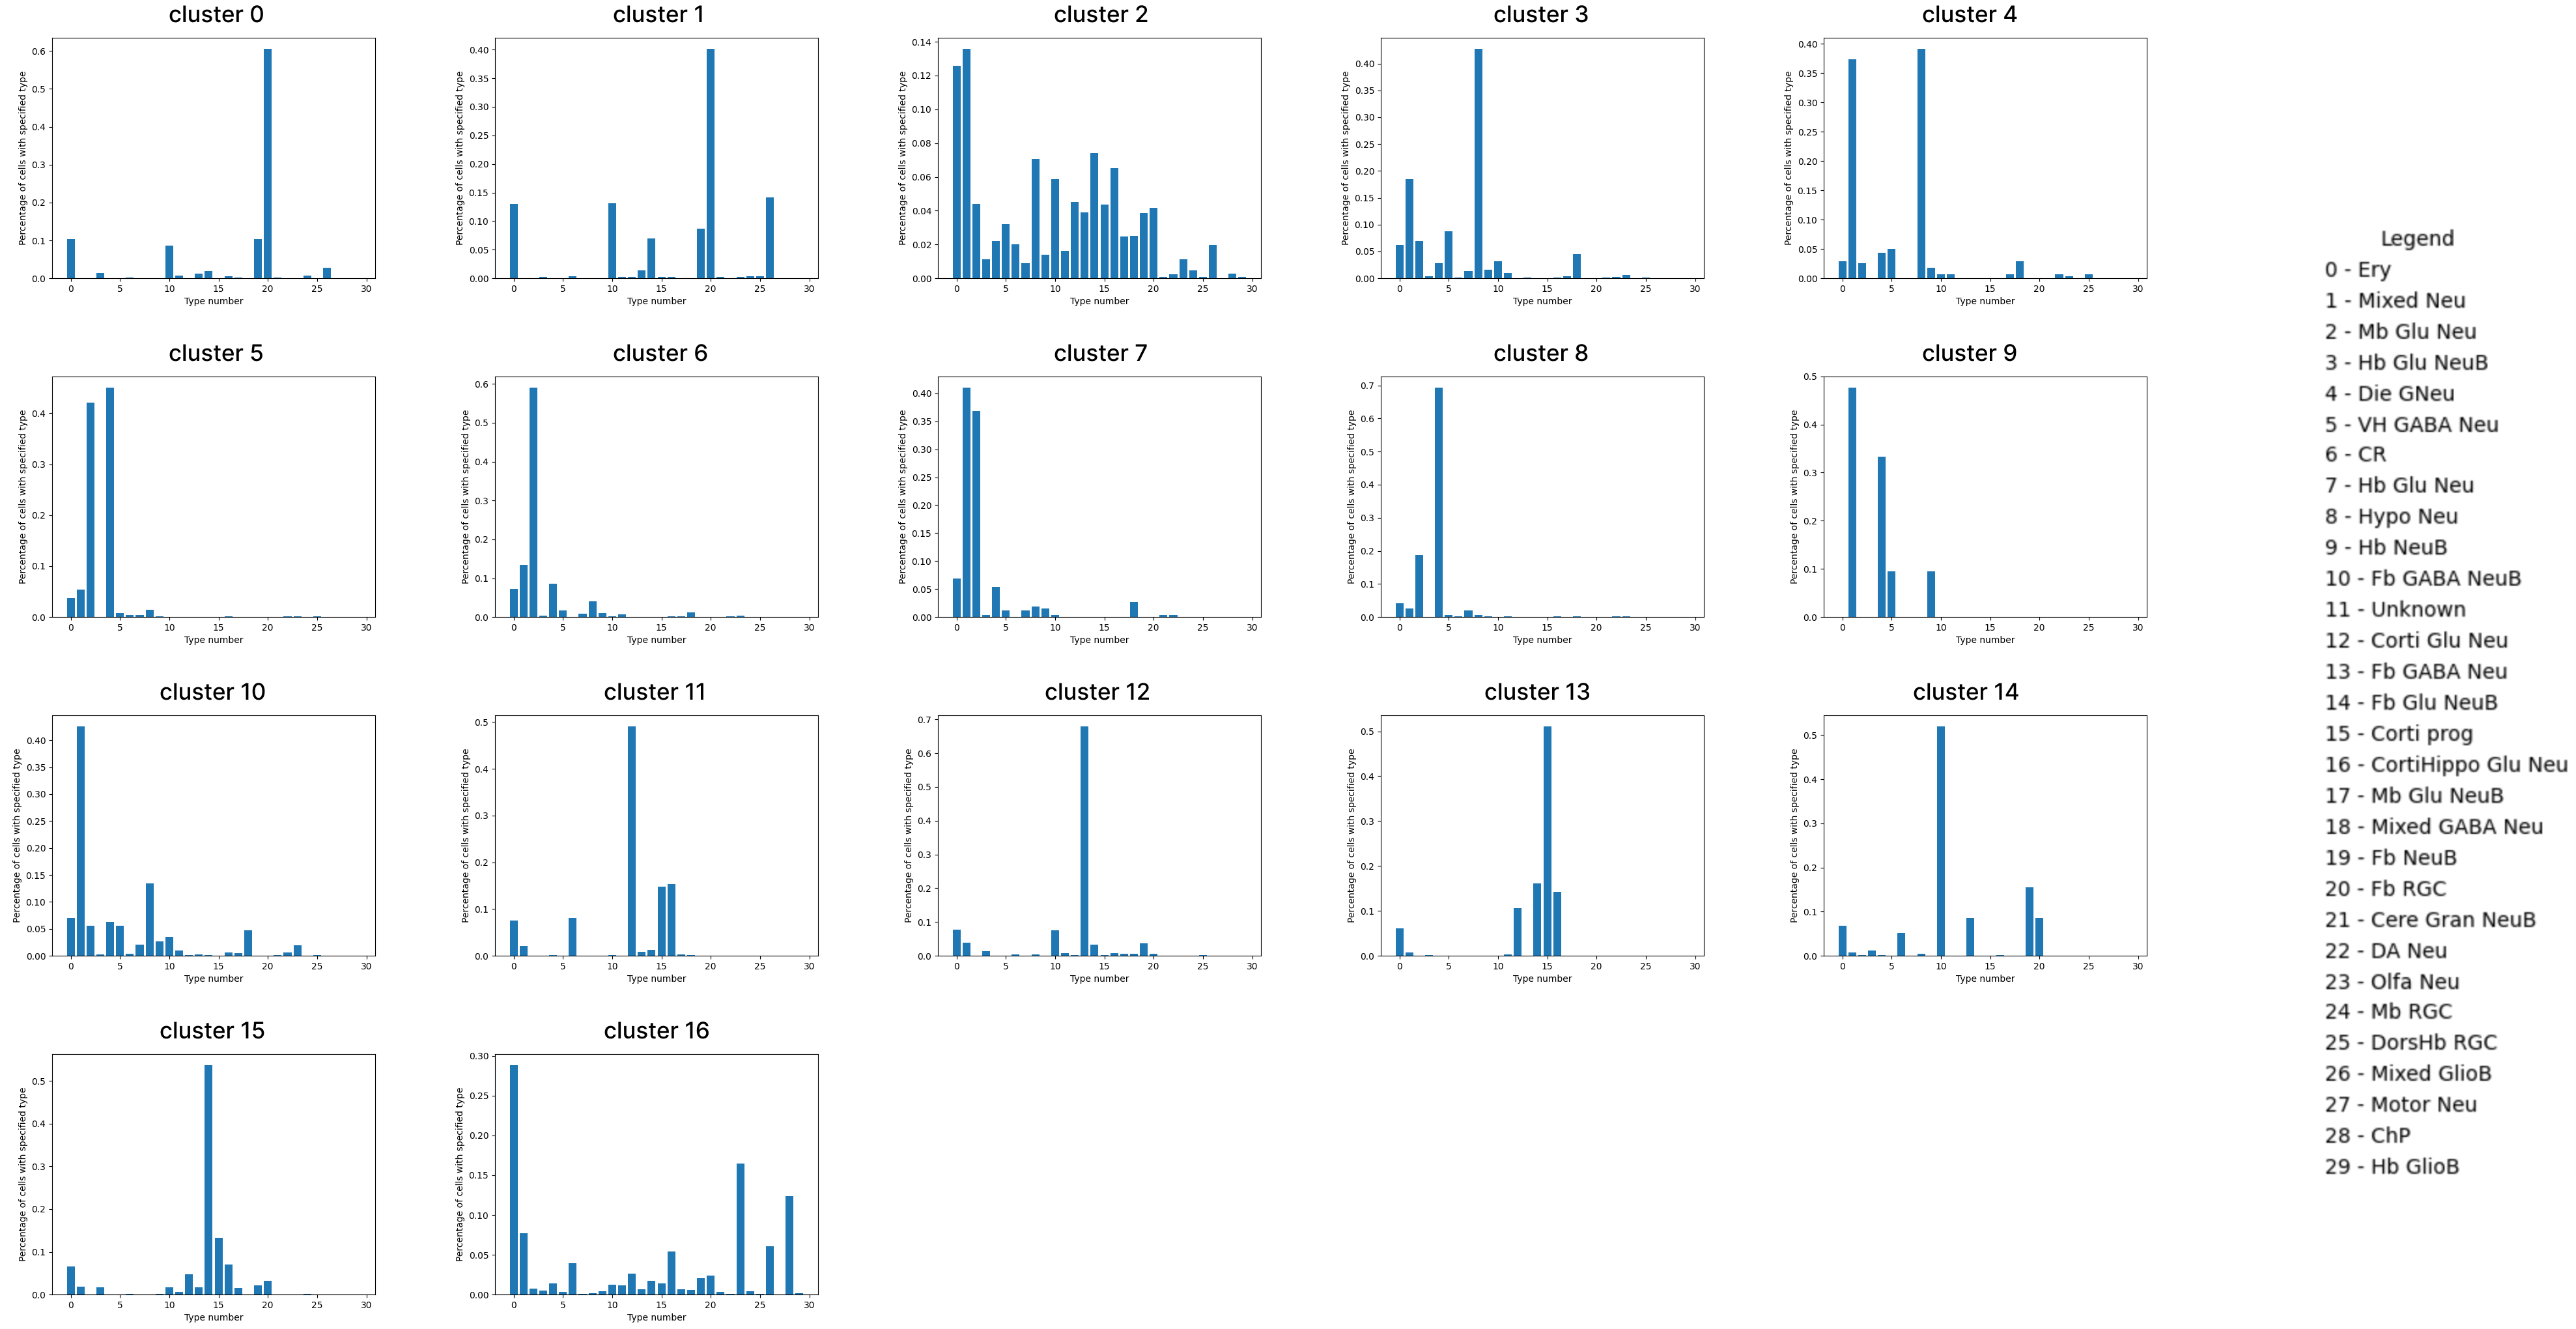
\includegraphics[width=1\textwidth]{type_p_clusters5.png}
    \caption{Percentage of different cell types in each cluster}
\end{figure} 

\end{frame}
%%%%%%%%%%%%%%%%%%%%%%%%%%%%%%%%%%%%%%%%%%%%%%%%%%%%%%%%%%%%%%%%%%%%%%%%%%%%%%
%%%%%%%%%%%%%%%%%%%%%%%%%%%%%%%%%%%%%%%%%%%%%%%%%%%%%%%%%%%%%%%%%%%%%%%%%%%%%%




\begin{frame}{Result 3 - Increasing the threshold}
\begin{itemize}
   \item<1-> []
   \begin{figure}
    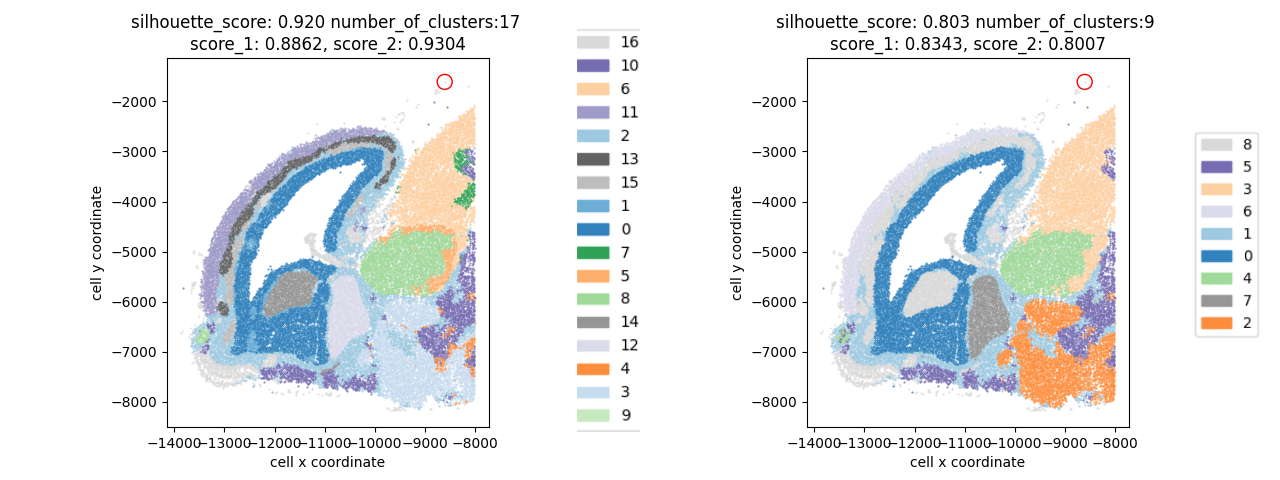
\includegraphics[width=0.6\textwidth]{clusters_4_5.png}
    \caption{Clusters with \texttt{threshold} $30$ and $45$, respectively}
\end{figure} 
    \item<2-> Increasing the threshold (from $30$ to $45$) did result in a lower number of clusters with slightly lower silhouette and total homogeneity score
    \item<3-> Clusters $0$ and $1$ from the previous clustering has now been merged into single cluster $0$. This has resulted in higher homogeneity score for cluster $0$ ($0.91$) than what was observed for cluster$1$ ($0.45$) and slightly lower score than $0$ ($1$) in the previous clustering 
\end{itemize}


\end{frame}
%%%%%%%%%%%%%%%%%%%%%%%%%%%%%%%%%%%%%%%%%%%%%%%%%%%%%%%%%%%%%%%%%%%%%%%%%%%%%%
\begin{frame}{Result 3 - Increasing the threshold}
\begin{itemize}
    \item<1-> []
    \begin{figure}
    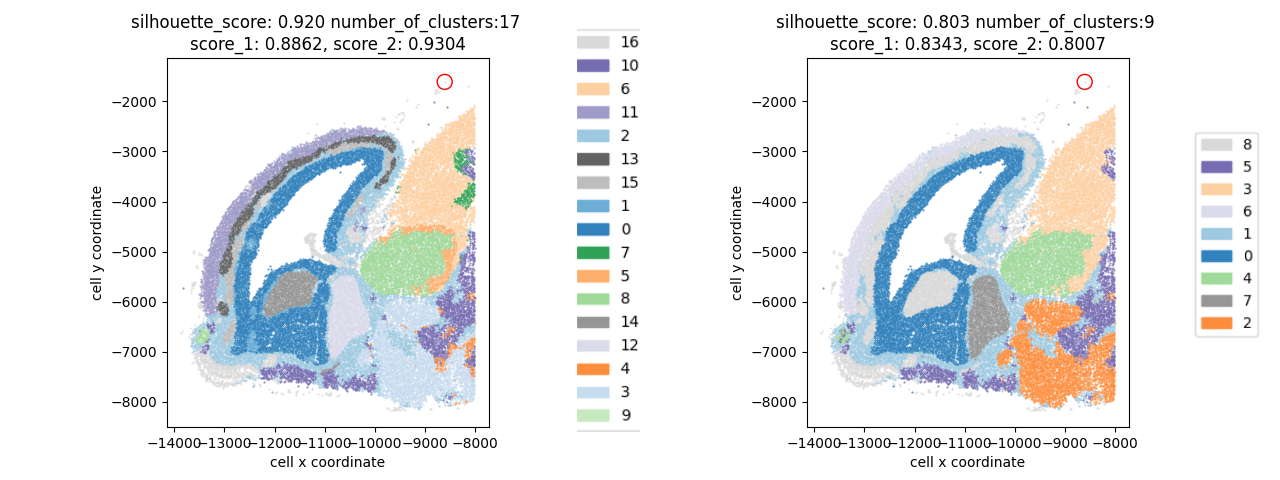
\includegraphics[width=0.6\textwidth]{clusters_4_5.png}
    \caption{Clusters with \texttt{threshold} $30$ and $45$, respectively}
\end{figure} 
     \item<2-> Clusters $13$ and $14$  and $15$ from the previous clustering has now been merged into clusters $8$. This  has resulted in lower homogeneity score for clusters $8$ ($0.07$) than what was observed for the clusters $13$ ($0.83$), $14$ ($0.92$) and $15$ ($1$) in the previous clustering. 
\end{itemize}


\end{frame}
%%%%%%%%%%%%%%%%%%%%%%%%%%%%%%%%%%%%%%%%%%%%%%%%%%%%%%%%%%%%%%%%%%%%%%%%%%%%%%
\begin{frame}{Result 3 - Increasing the threshold}

\begin{figure}
    \centering
    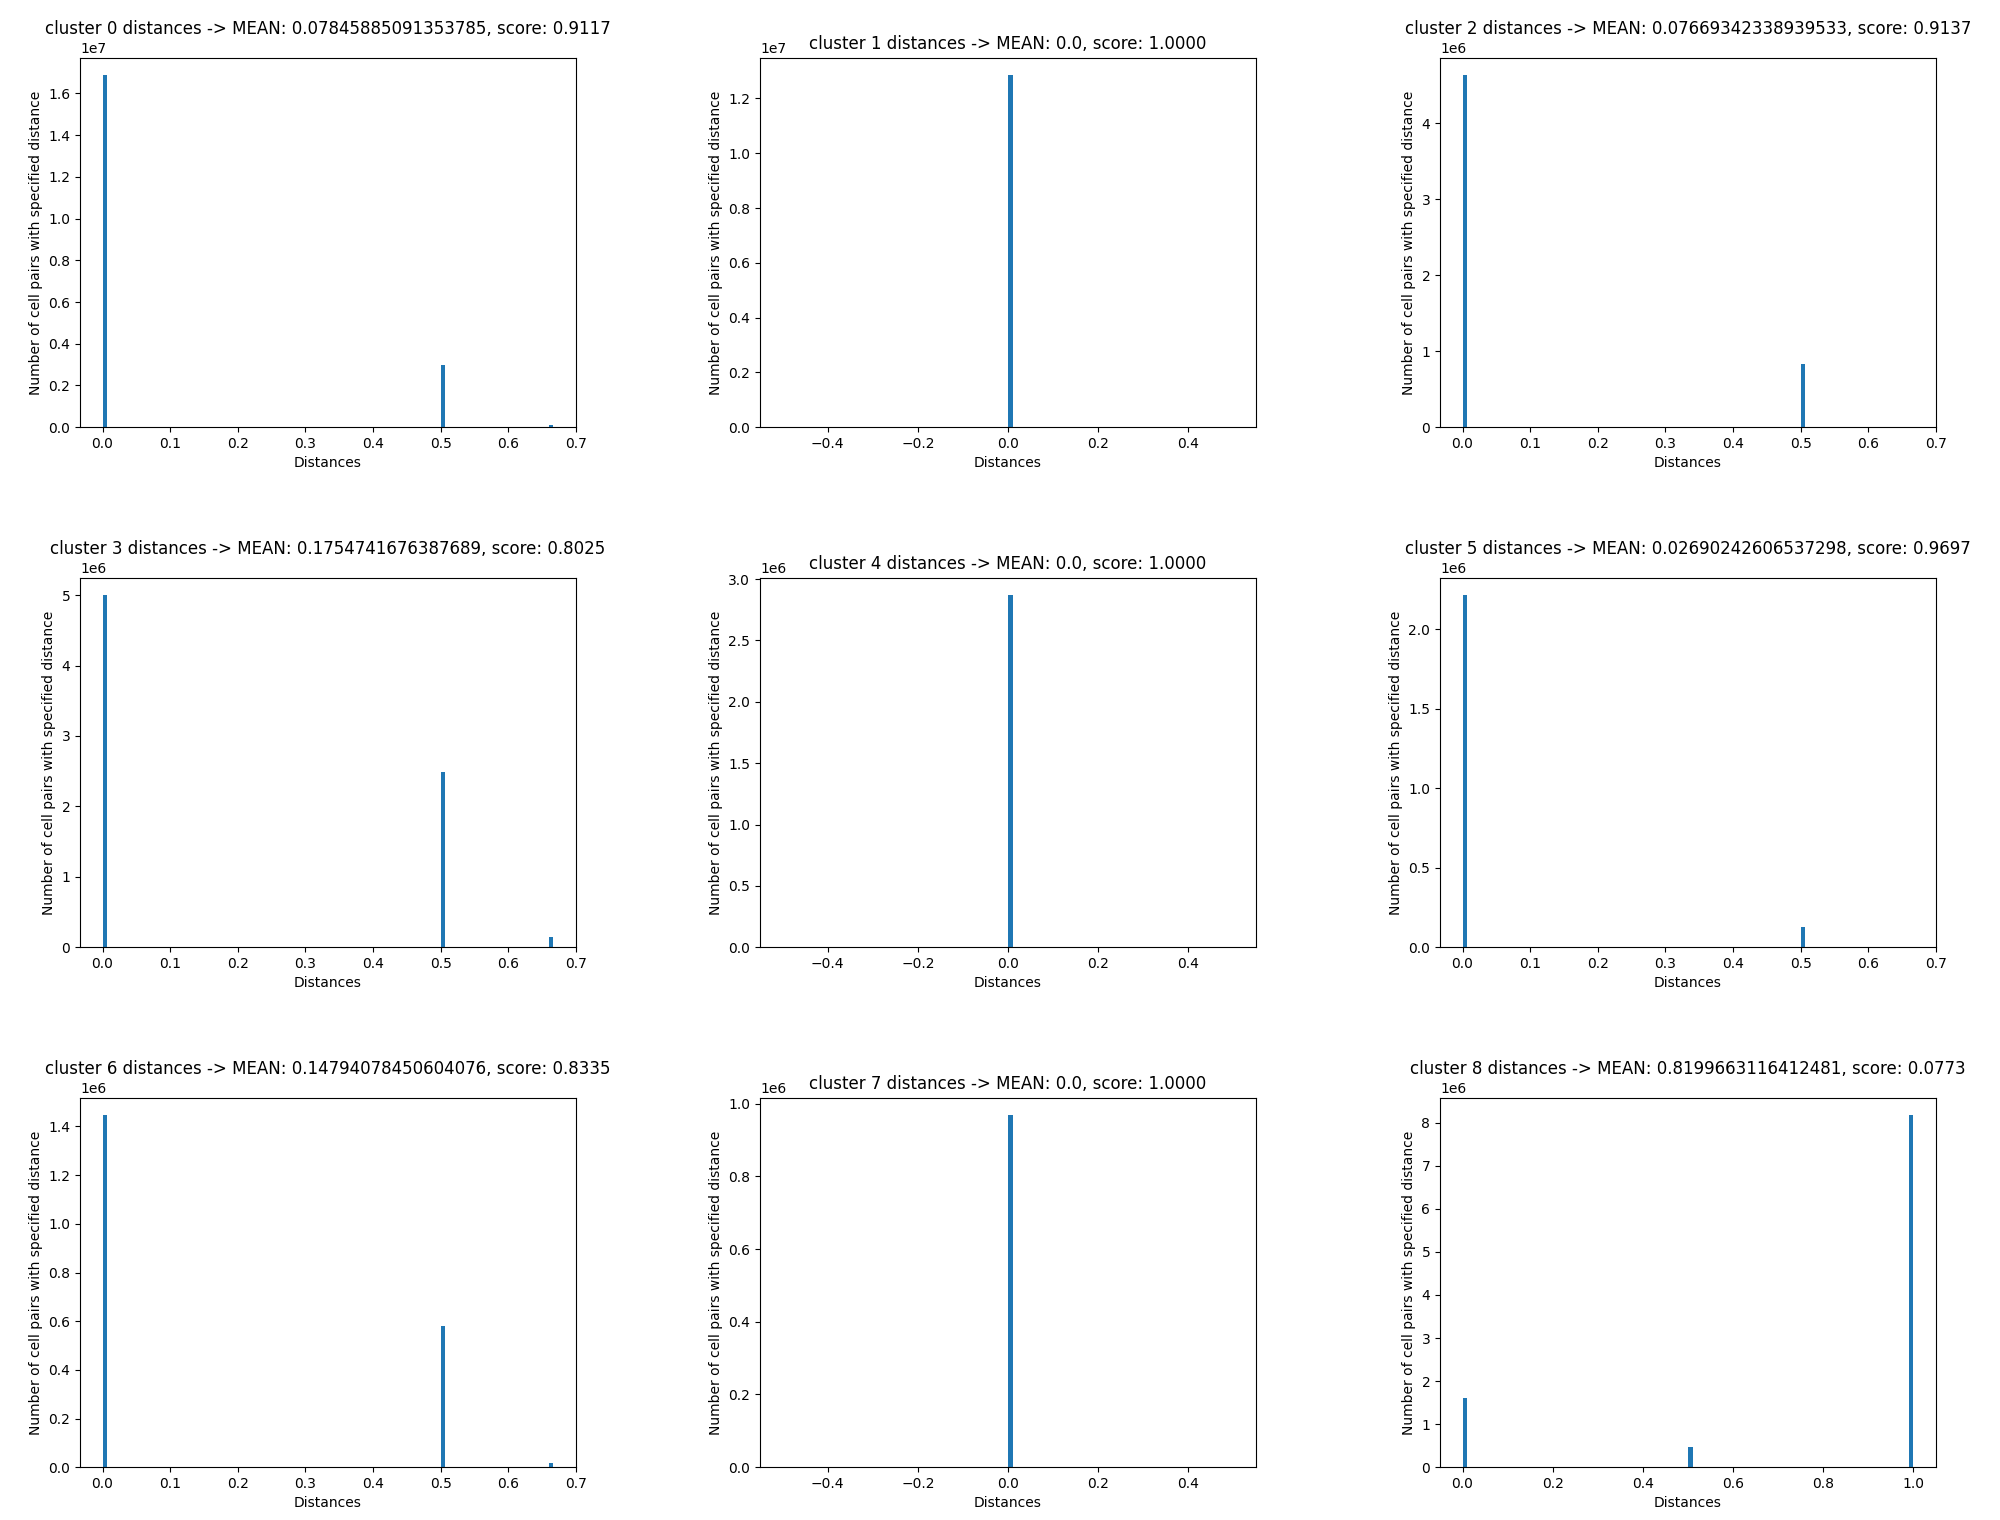
\includegraphics[width=0.8\textwidth]{stats_clusters6.png}
    \caption{Distribution of percentage distances between cells for each cluster}
\end{figure} 

\end{frame}

%%%%%%%%%%%%%%%%%%%%%%%%%%%%%%%%%%%%%%%%%%%%%%%%%%%%%%%%%%%%%%%%%%%%%%%%%%%%%%
\begin{frame}{Result 3 - Increasing the threshold}

\begin{figure}
    \centering
    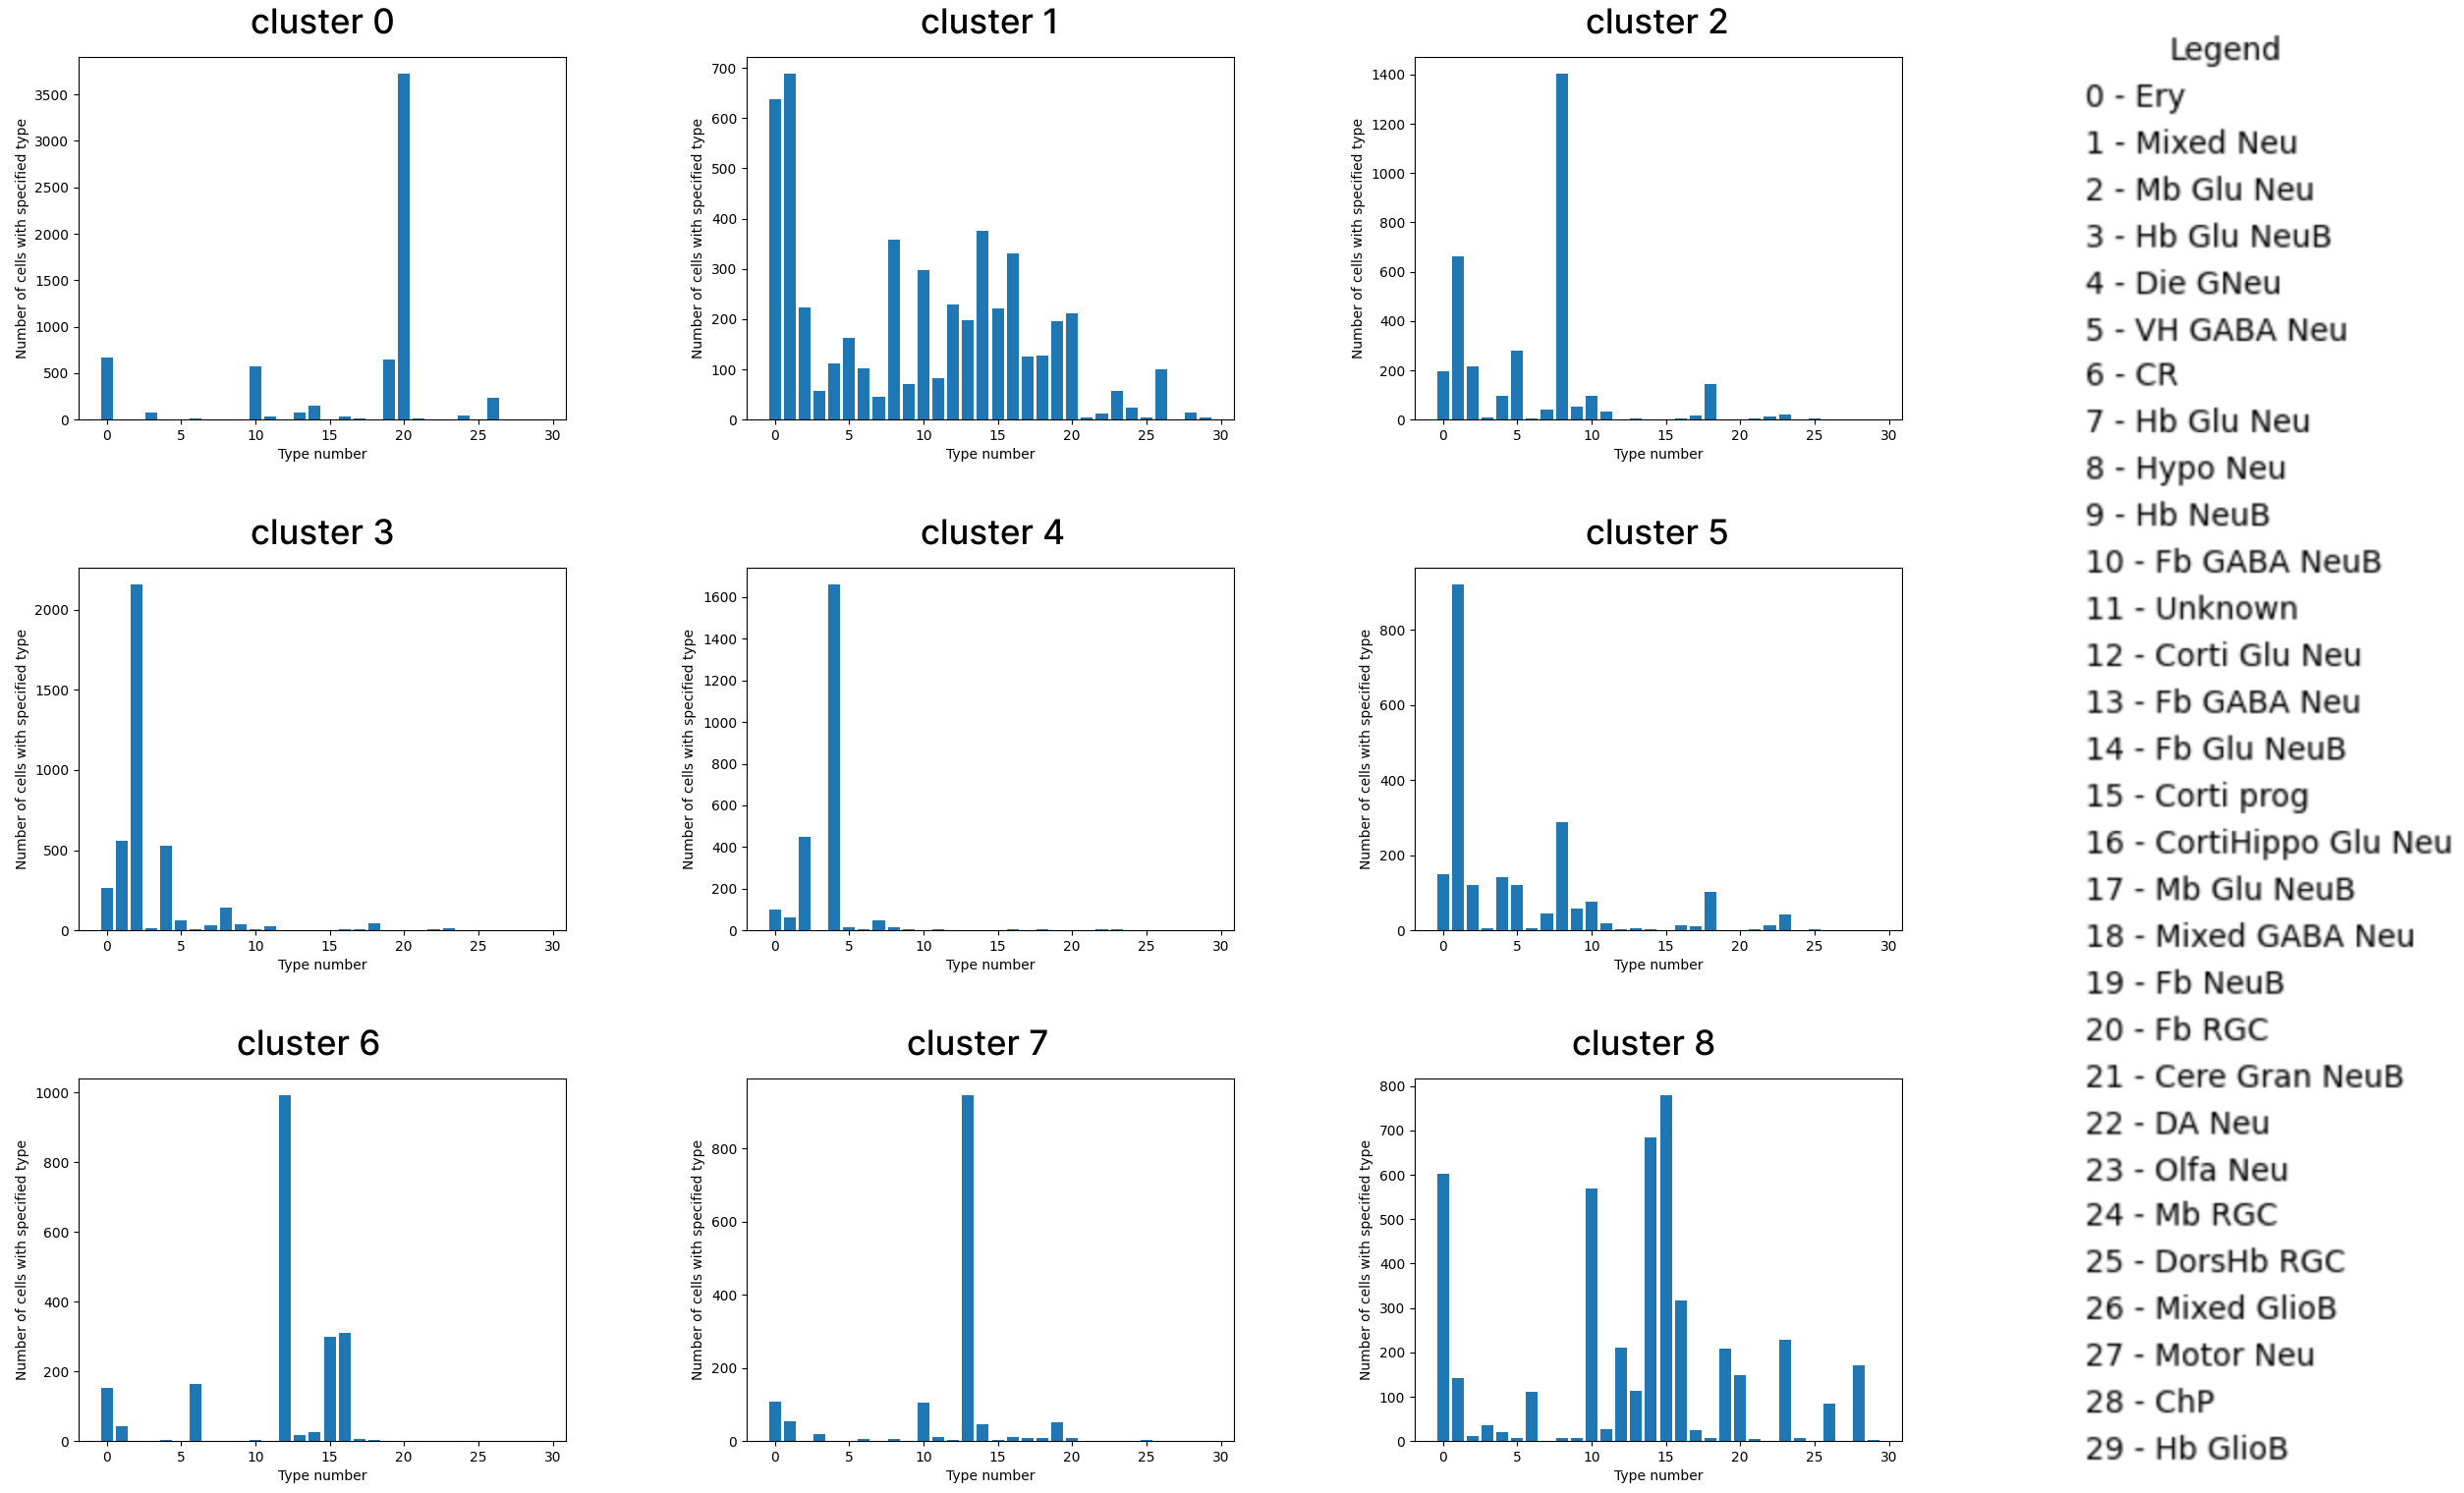
\includegraphics[width=0.8\textwidth]{type_num_clusters6.png}
    \caption{Number of different cell types in each cluster}
\end{figure} 

\end{frame}
%%%%%%%%%%%%%%%%%%%%%%%%%%%%%%%%%%%%%%%%%%%%%%%%%%%%%%%%%%%%%%%%%%%%%%%%%%%%%%
\begin{frame}{Result 3 - Increasing the threshold}

\begin{figure}
    \centering
    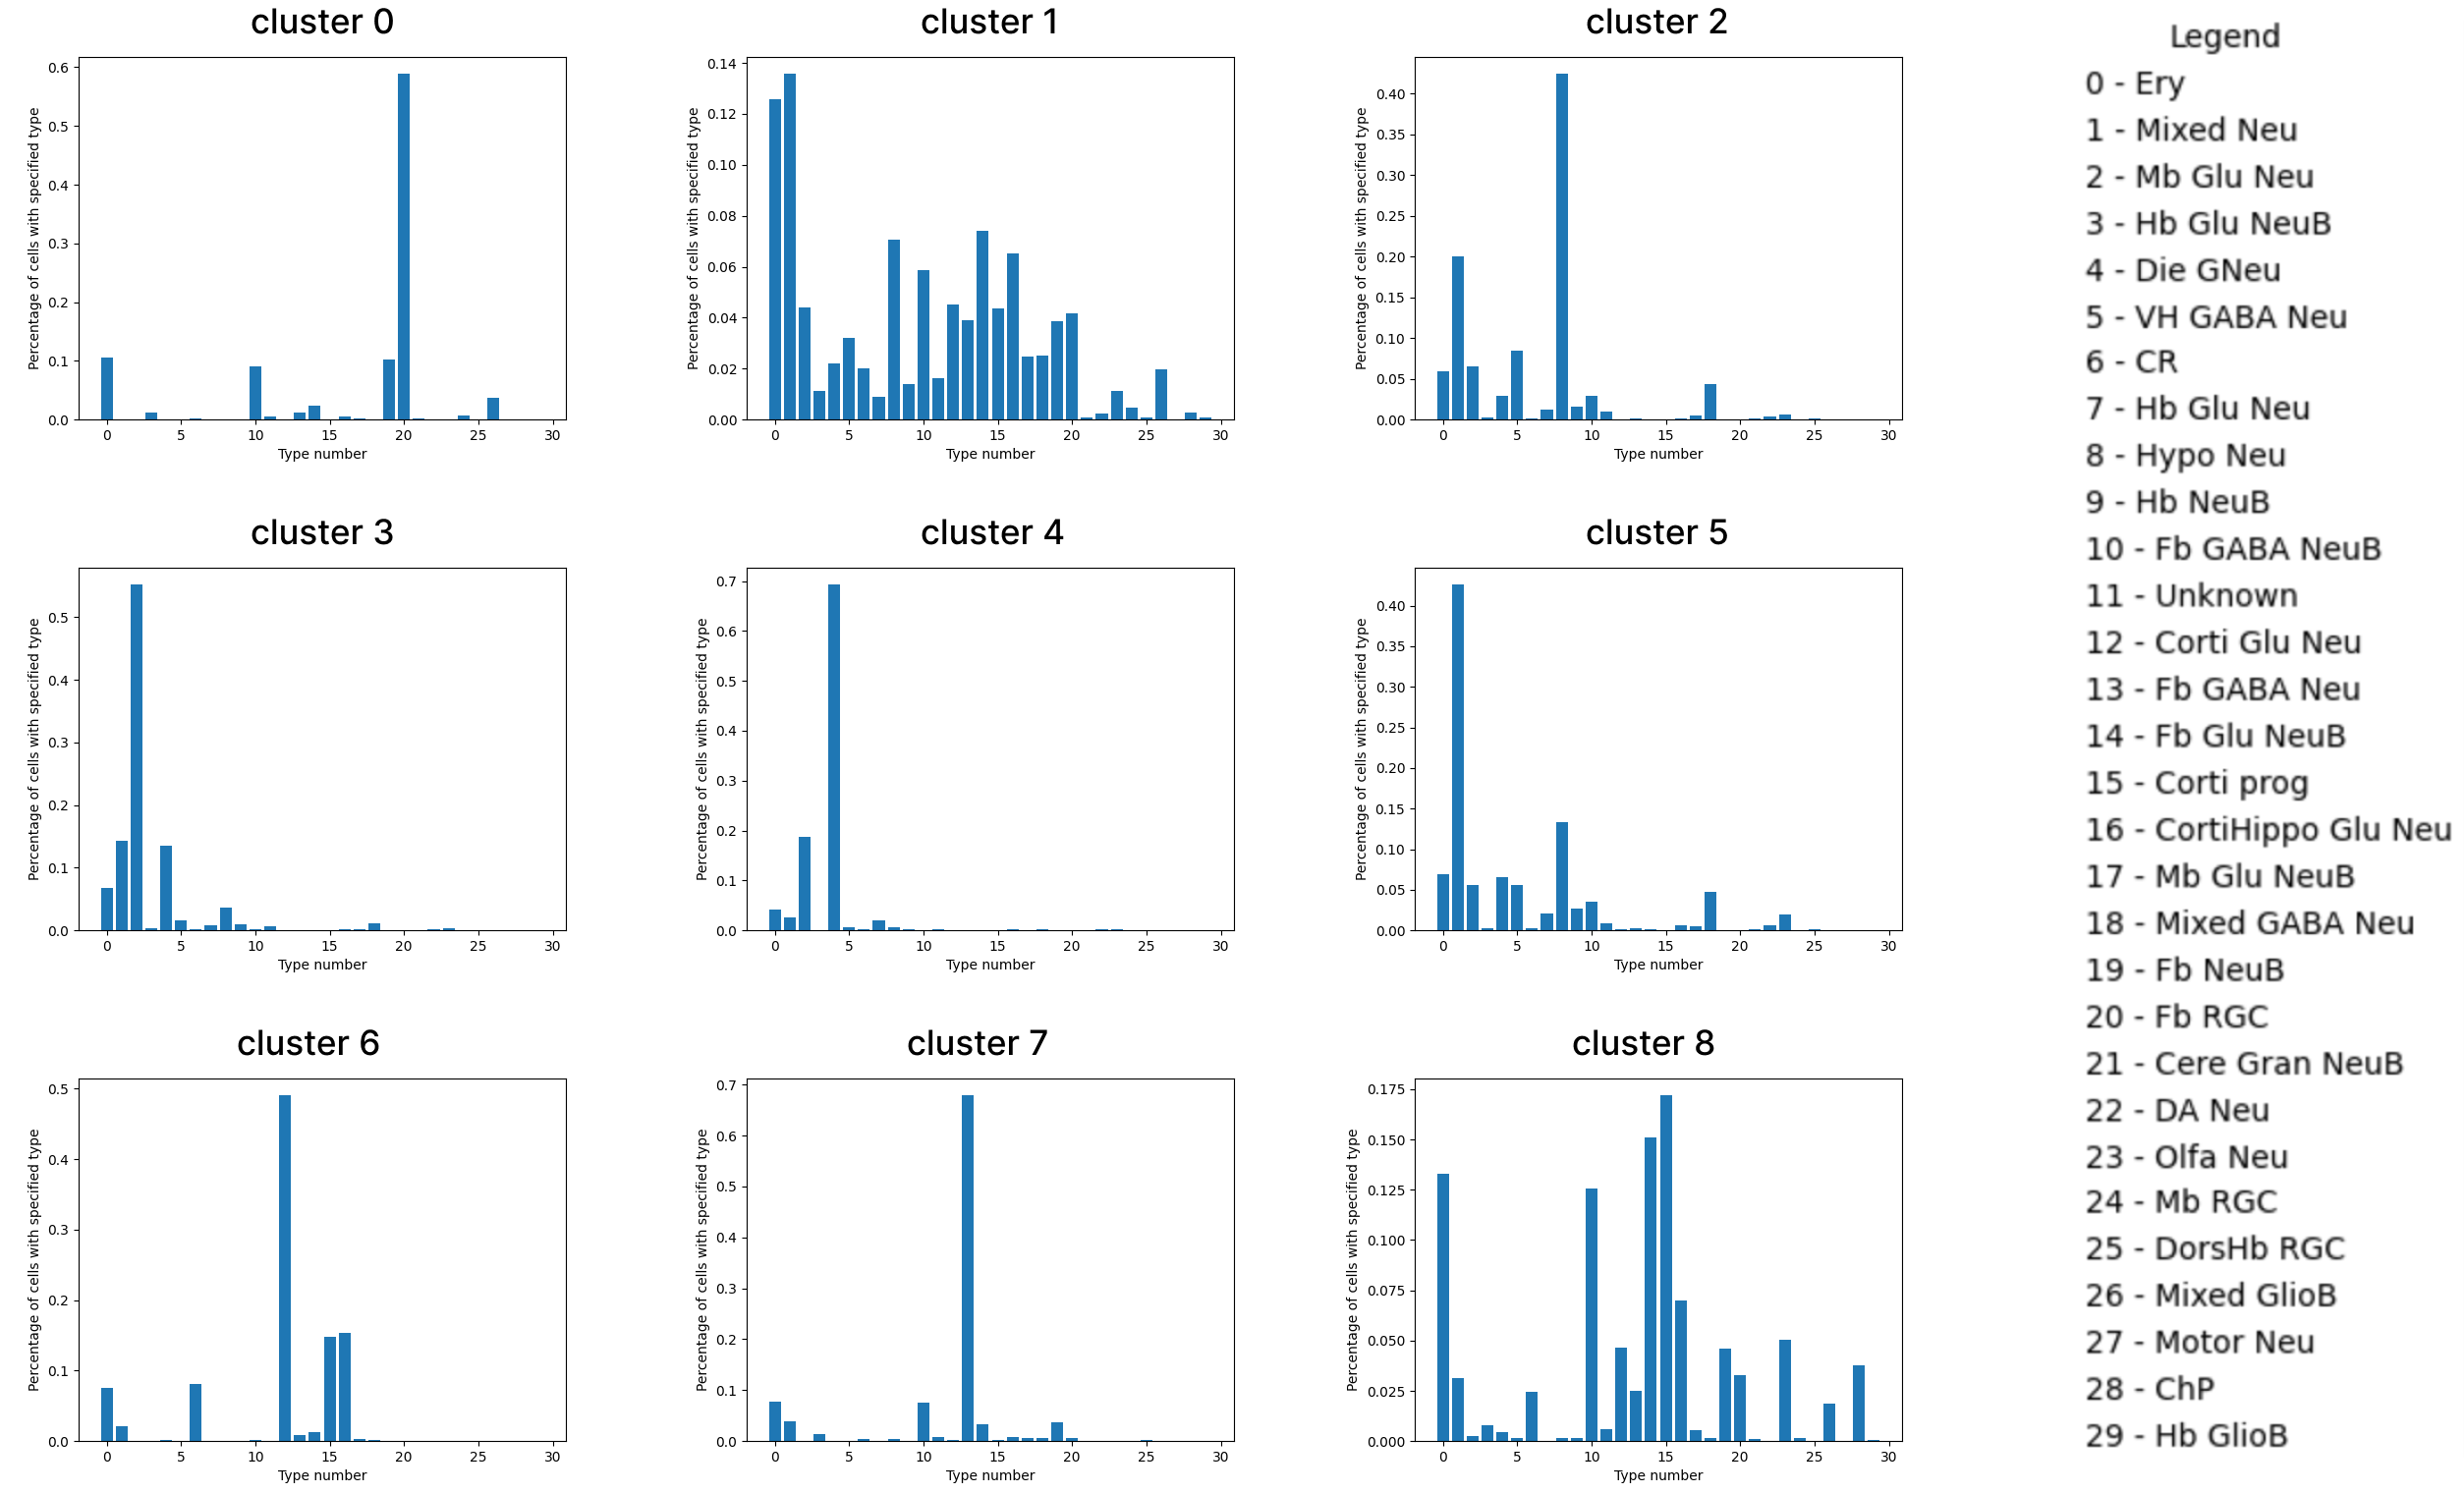
\includegraphics[width=0.8\textwidth]{type_p_clusters6.png}
    \caption{Percentage of different cell types in each cluster}
\end{figure} 

\end{frame}
%%%%%%%%%%%%%%%%%%%%%%%%%%%%%%%%%%%%%%%%%%%%%%%%%%%%%%%%%%%%%%%%%%%%%%%%%%%%%%




%%%%%%%%%%%%%%%%%%%%%%%%%%%%%%%%%%%%%%%%%%%%%%%%%%%%%%%%%%%%%%%%%%%%%%%%%%%%%%
%%%%%%%%%%%%%%%%%%%%%%%%%%%%%%%%%%%%%%%%%%%%%%%%%%%%%%%%%%%%%%%%%%%%%%%%%%%%%%
\subsection{Conclusion}
\begin{frame}{Conclusion}

\begin{figure}
    \centering
    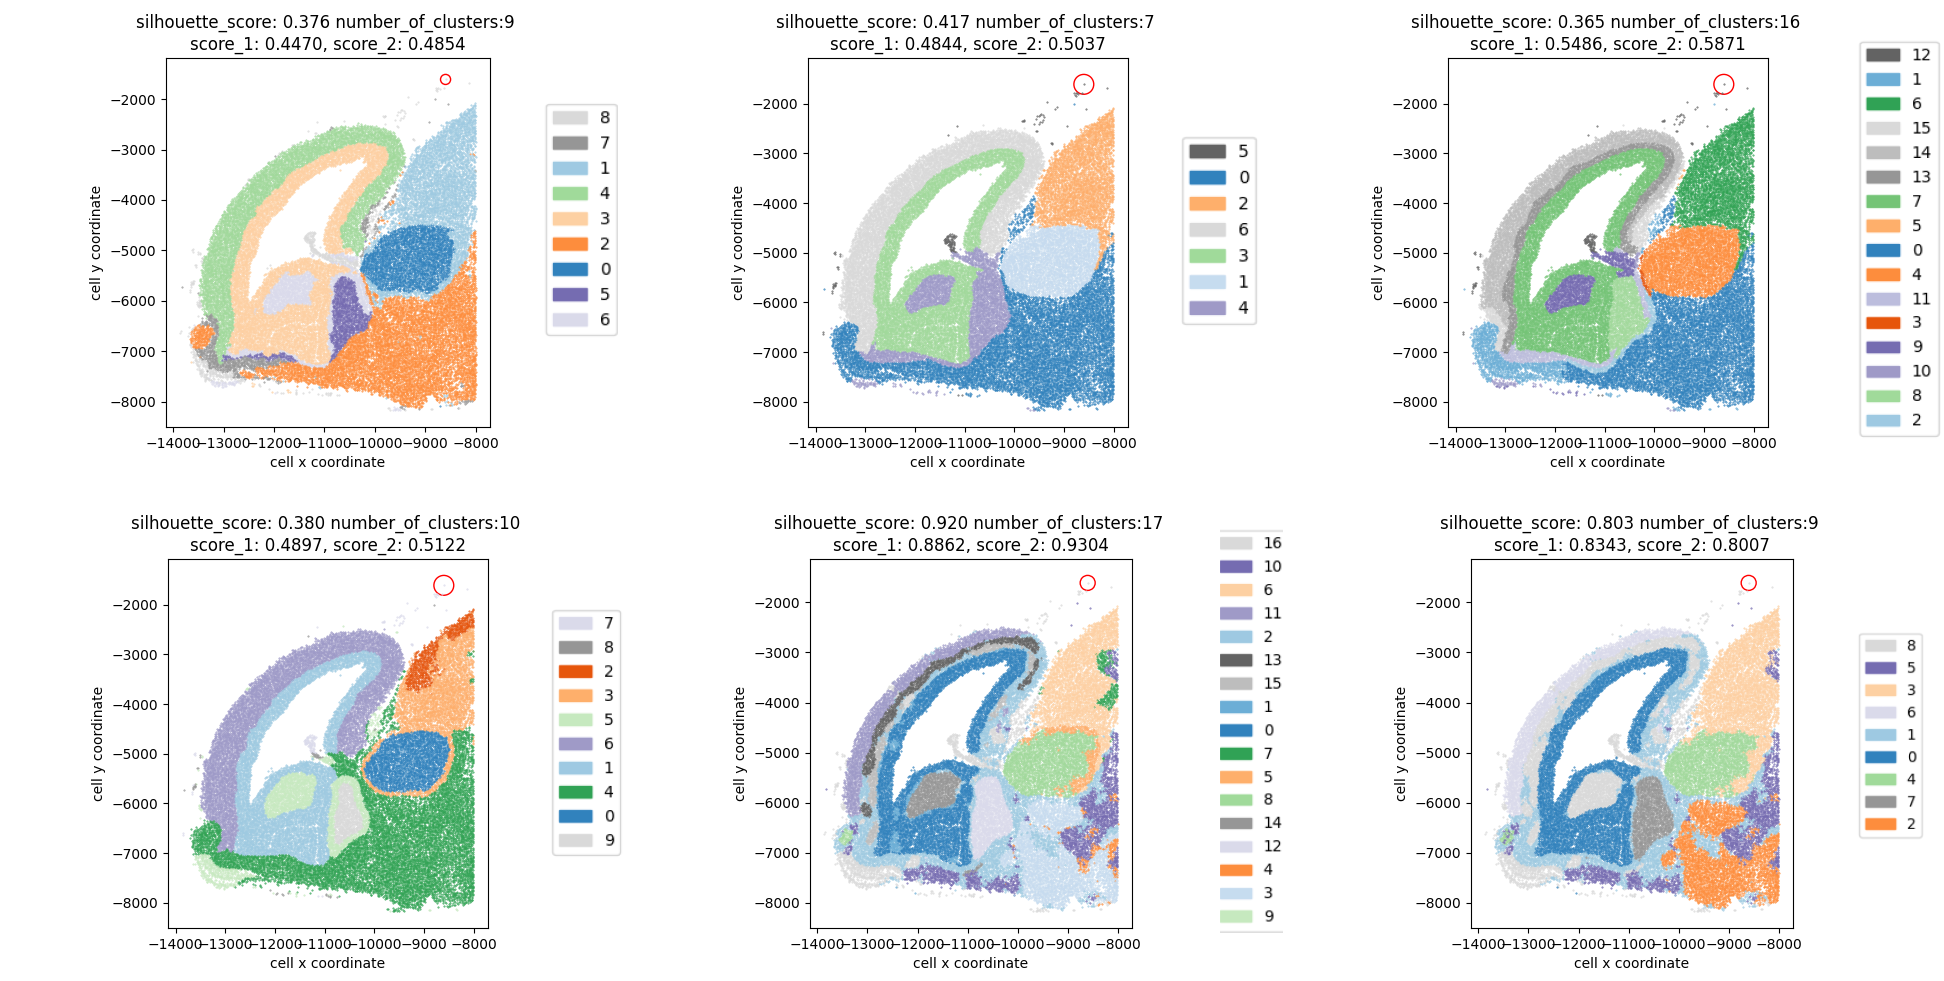
\includegraphics[width=0.8\textwidth]{all_clusters.png}
    \caption{Clusters for different clusterings - Manhattan ($100$ & $200$ - different threshold), Euclidean ($200$) & Hamming with parameter $0.3$ ($150$ - different thresholds)}
\end{figure} 

\end{frame}
%%%%%%%%%%%%%%%%%%%%%%%%%%%%%%%%%%%%%%%%%%%%%%%%%%%%%%%%%%%%%%%%%%%%%%%%%%%%%%

\begin{frame}{Conclusion}

\begin{itemize}
    \item<1-> From the image above, it is evident that several homogeneous clusters are consistently present in almost all of the different clusterings:
        \begin{itemize}
            \item<2-> $0$, $1$, $4$, $0$,  $8$ and $4$
            \item<3-> $5$, $8$, $9$, $12$ and $7$
            \item<4-> $3$, $3$, $7$, $1$,  $0$ and $0$
            \item<5-> $1$, $2$, $6$, $3$,  $6$ and $3$
        \end{itemize}
    \item<6-> Furthermore, there are clusters that appear as a single cohesive group in one clustering but get divided into smaller, more homogeneous sub-clusters in others
\end{itemize}

\end{frame}
%%%%%%%%%%%%%%%%%%%%%%%%%%%%%%%%%%%%%%%%%%%%%%%%%%%%%%%%%%%%%%%%%%%%%%%%%%%%%%









%%%%%%%%%%%%%%%%%%%%%%%%%%%%%%%%%%%%%%%%%%%%%%%%%%%%%%%%%%%%%%%%%%%%%%%%%%%%%%
\section{Projects}
\begin{frame}{Projects}

\begin{itemize}
    \item<1-> Algorithms for DNA sequencing
    \begin{itemize}
    \item<2-> [] Wrote course on algorithms for DNA sequencing for Faculty of Mathematics’ educational software
    \end{itemize}
    \item<3-> Success of ICD therapy - Prediction of death due to heart problems
    \begin{itemize}
    \item<4-> [] Tried to find parameters of the clinical picture of patients that would potentially lead to a better prediction of death due to heart problems
    \end{itemize}
    \item<5-> MSc thesis: Clustering data obtained through spatial transcriptomics techniques
    \begin{itemize}
    \item<6-> [] Investigated correlation between spatial coordinates and gene expressions of the cells while also analyzing their impact on cell type
    \end{itemize}
\end{itemize}

\end{frame}
%%%%%%%%%%%%%%%%%%%%%%%%%%%%%%%%%%%%%%%%%%%%%%%%%%%%%%%%%%%%%%%%%%%%%%%%%%%%%%


%%%%%%%%%%%%%%%%%%%%%%%%%%%%%%%%%%%%%%%%%%%%%%%%%%%%%%%%%%%%%%%%%%%%%%%%%%%%%%%
%%%%%%%%%%%%%%%%%%%%%%%%%%%%%%%%%%%%%%%%%%%%%%%%%%%%%%%%%%%%%%%%%%%%%%%%%%%%%%
%%%%%%%%%%%%%%%%%%%%%%%%%%%%%%%%%%%%%%%%%%%%%%%%%%%%%%%%%%%%%%%%%%%%%%%%%%%%%%%
%%%%%%%%%%%%%%%%%%%%%%%%%%%%%%%%%%%%%%%%%%%%%%%%%%%%%%%%%%%%%%%%%%%%%%%%%%%%%%


\end{document}
